% !TeX root = ./Lewandowski2018.tex
\documentclass[onecolumn]{svjour3}   
%\usepackage{amssymb,amsthm,mathrsfs,graphicx, bm}
\usepackage{amssymb,mathrsfs,graphicx, bm}
\usepackage{natbib}
\usepackage{subcaption}
% \usepackage{titlesec}
\usepackage{geometry}
\usepackage{fancyhdr}
\usepackage{newtxtext,newtxmath}
\usepackage{hyperref}

\usepackage{color}
\usepackage{amsfonts}
\pagenumbering{arabic}

%Packages for Matlab2TikZ
\usepackage{pgfplots}
\pgfplotsset{compat=newest}
\usetikzlibrary{plotmarks}
\usetikzlibrary{arrows.meta}
%\tikzset{every picture/.style={/utils/exec={\boldsymbol{\rm X}}{\sffamily}}}
\usepgfplotslibrary{patchplots}
\usepackage{grffile}

\usepackage{lineno,hyperref}
\usepackage{moreverb}
\usepackage[ruled,slide]{algorithm2e}



\begin{document}

\title{A computational framework for crack propagation in spatially heterogeneous materials}
\subtitle{}
\author{Karol Lewandowski \and
	{\L}ukasz Kaczmarczyk \and
	Ignatios Athanasiadis \and
	John F. Marshall\and 
	Chris J. Pearce 
}

\institute{Karol Lewandowski \at
	Glasgow Computational Engineering Centre, The James Watt School of Engineering, University of Glasgow, Glasgow, G12 8QQ, UK \\
	\email{karol.lewandowski@glasgow.ac.uk}           %  \\
	\and
	John F. Marshall \at
	Weipers Centre Equine Hospital, School of Veterinary Medicine, University of Glasgow, Glasgow, G61 1QH, UK
} 

\date{Received: date / Accepted: date}

\maketitle
% \author[gla,vet]{Karol Lewandowski\corref{cor}}
% \ead{karol.lewandowski@glasgow.ac.uk}
% \author[gla]{{\L}ukasz Kaczmarczyk}
% \ead{lukasz.kaczmarczyk@glasgow.ac.uk}
% \author[gla]{Ignatios Athanasiadis}
% \ead{ignatios.athanasiadis@glasgow.ac.uk}
% \author[vet]{John F. Marshall}
% \ead{john.f.marshall@glasgow.ac.uk}
% \author[gla]{Chris J. Pearce}
% \ead{chris.pearce@glasgow.ac.uk}
% \cortext[cor]{Corresponding author}
% \address[gla]{Glasgow Computational Engineering Centre, The James Watt School of Engineering, University of Glasgow, Glasgow, G12 8QQ, UK.}
% \address[vet]{Weipers Centre Equine Hospital, School of Veterinary Medicine, University of Glasgow, Glasgow, G61 1QH, UK,}

\begin{abstract}
This paper presents a mathematical formulation and numerical modelling framework for brittle crack propagation in heterogeneous elastic solids. 
Such materials are present in both natural and engineered scenarios.
The formulation is developed in the framework of configurational mechanics and solved numerically
using the finite element method.
We show that the methodology previously established for homogeneous materials without the need for any further assumptions. 
The proposed model is based on the assumption of maximal dissipation of energy and utilises the Griffith criterion; we 
show that this is sufficient to predict crack propagation in brittle heterogeneous materials, with spatially varying Young's modulus and fracture energy.
Furthermore, we show that the crack path trajectory orientates itself such that it is always subject to Mode-I. 
The configurational forces and fracture energy release rate are both expressed exclusively in terms of nodal quantities, 
avoiding the need for post-processing and enabling a fully implicit formulation for modelling the evolving crack front and creation of new crack surfaces.
The proposed formulation is verified and validated by comparing numerical results with both analytical solutions and experimental results.
Both the predicted crack path and load-displacement response show very good agreement with experiments where the crack path was independent of material heterogeneity for those cases.
Finally, the model is successfully used to consider the real and challenging scenario of fracture of an equine bone, with spatially varying material properties obtained from CT scanning. 


\keywords{ Finite element analysis \and functionally graded materials  \and fracture  \and configurational mechanics  \and heterogeneous materials}
\end{abstract}


%\linenumbers

\section{Introduction}
% 
% 
The predictive modelling of crack propagation continues to generate significant scientific interest and 
represents an ongoing focus for computational mechanics research.  
The unstable and highly nonlinear nature of crack propagation in three-dimensional solids
means that the development of a robust and objective modelling capability, 
that is able to capture the evolution of the crack front and creation of new crack surfaces, represents a considerable challenge.

This paper extends the authors' previous work for brittle fracture in solids that comprise homogeneous materials~\cite{kaczmarczyk2017energy}, 
to now consider spatially heterogenous materials. 
Such materials are prevalent in both natural and engineered materials. 
Functionally Graded Materials (FGM) is a class of materials whose composition (and therefore material properties) 
vary spatially in a smooth fashion \cite{KawasakiWatanabe1997} and are used in many engineering 
applications \cite{Jha2013, NaebeShirvan2016}.
The advantage of FGMs is that they can be designed to achieve desired mechanical behaviour \cite{Erdogan1995, FinotSuresh1996}. 
Nevertheless, it is necessary to model their behaviour and failure characteristics when used in critical engineering applications. 
Numerical models have been proposed to investigate crack propensity and stress intensity factors in FGMs for various material distribution 
and multiple cracks, for instance \cite{KimPaulino2002, Ayhan2009, ZhangBEM2011, ShiMan2014, ShojaeeDaneshmand2015}. 
Despite the breadth and importance of applications where these materials are present, 
numerical modelling of crack propagation is still in the early stages of development.
The majority of well validated models available are limited to 2D analysis \cite{KimPaulino2004,Bayesteh2013, Ooi2015, Chafi2019}.
For the 3D case, a phase field model has also been proposed \cite{Hirshikesh2019}.
However, such an approach is strongly mesh-size and step-size dependent, 
which could present an unsurmountable computational challenge for full scale  applications.

Natural materials, such as bamboo, bone and skin exhibit spatially heterogenous materials that also evolve over time. 
In particular, bone adapts to its mechanical environment (commonly referred to as bone remodelling); 
this is an on-going biological process of replacing old bone tissue with new bone, thus repairing fatigue damage~\cite{hughes2017role}. 
This ability to repair bone micro-damage is essential for maintaining mechanical integrity. 
Therefore, variations in bone tissue quality and hence material properties can be observed at different locations and times of bone life. 
Consequently, there is a strong correlation between stress fractures and the adaptation process~\cite{hughes2017role}. 
Furthermore, bone repair can be overwhelmed by load-induced bone densification that also increases brittleness and reduces fracture resistance~\cite{loughridge2017qualitative}.

This paper addresses the need for an energetically consistent model for crack propagation in heterogeneous materials.
The formulation is developed in the framework of configurational mechanics and solved numerically using the finite element method.
The concept of configurational forces was originally introduced by Eshelby~\cite{eshelby1951force}. 
Unlike physical forces, configurational forces act on the material manifold and represent the tendency of imperfections like cracks, 
voids or material inhomogeneities to move relative to the surrounding material. 
The past two decades have seen a growing interest in this approach for analysis of material imperfections~\cite{maugin2016configurational} and in particular for evaluating the forces driving crack advancement~\cite{kaczmarczyk2017energy,steinmann2001application, ozencc2016configurational}. 
However, until recently this approach has never been used to effectively assess configurational forces for cracking in heterogeneous bodies. 

The model presented in this paper is based on the assumption of maximal dissipation of energy and utilises the Griffith criterion. 
We show that these assumptions are sufficient to predict crack propagation in brittle heterogeneous materials, 
using configurational mechanics. 
Additional configurational forces, arising from inhomogeneities~\cite{kienzler2014configurational}
associated with spatially varying properties are introduced into the formulation. This allows for both the accurate assessment of the likelihood of a crack to propagate and to simulate the subsequent propagation of fractures. 
The model offers a computationally efficient 3D analysis tool for complex materials by means of a monolithic approach 
with relatively small number of finite elements.

\textcolor{red}{Furthermore, the focus of this work is on the modelling of physical processes arising from crack propagating through material heterogeneity and \emph{not} on the particular choice of displacement jump approximation approach along the crack path.}
\textcolor{red}{{The framework proposed is not restricted to the underlying crack propagation implementation of the present work i.e. mesh cutting algorithm.
Other popular brittle crack propagation approaches such as XFEM and PUFEM, \citep{Belytschko1999, WriggersXFEM, Babuska2017, Tian2019}} could adopt the present framework by adding explicit approximation of material position to incorporate configurational forces evaluation.  }

This article is structured as follows. After establishing the kinematic preliminaries in Section~\ref{preliminaries}, Section~\ref{sec:fracture_prop} extends the authors' previous work for evolving crack propagation within the framework of configurational mechanics. Section \ref{sec:fem_modelling} describes the finite element method implementation and briefly introduces a special element for capturing the singular stress field at the crack front.  
All the above components are brought together into a single framework and its performance is demonstrated using a series of numerical examples in Section~\ref{sec:numerical_examples}, where the model is validated with experimental results for 
FGMs, as well as applying it to a full-scale model of equine bones using clinically available CT-scanning data.


% 
% 
\section{Preliminaries}
\label{preliminaries}
Figure~\ref{fig:domains4} shows a section of a solid with an initial crack in the reference domain $\mathscr{B}_{0}$. As a result of loading, the crack extends and the body deforms elastically. Working within the framework of configurational mechanics \cite{kaczmarczyk2014three,kienzler2014configurational}, it is convenient to decompose this behaviour into an extension of the crack in the material domain  $\mathscr{B}_t$ followed by elastic deformation in the spatial domain $\Omega_t$. The former is described by the mapping from the reference  domain to the material domain ${\boldsymbol\Xi}$, whilst the latter is described by the mapping from the material to the spatial domain ${\boldsymbol\varphi}$ - Figure~\ref{fig:domains4}.

\begin{figure}[th] 
\setlength{\fboxsep}{0pt}%
\setlength{\fboxrule}{0pt}%
\begin{center}
% 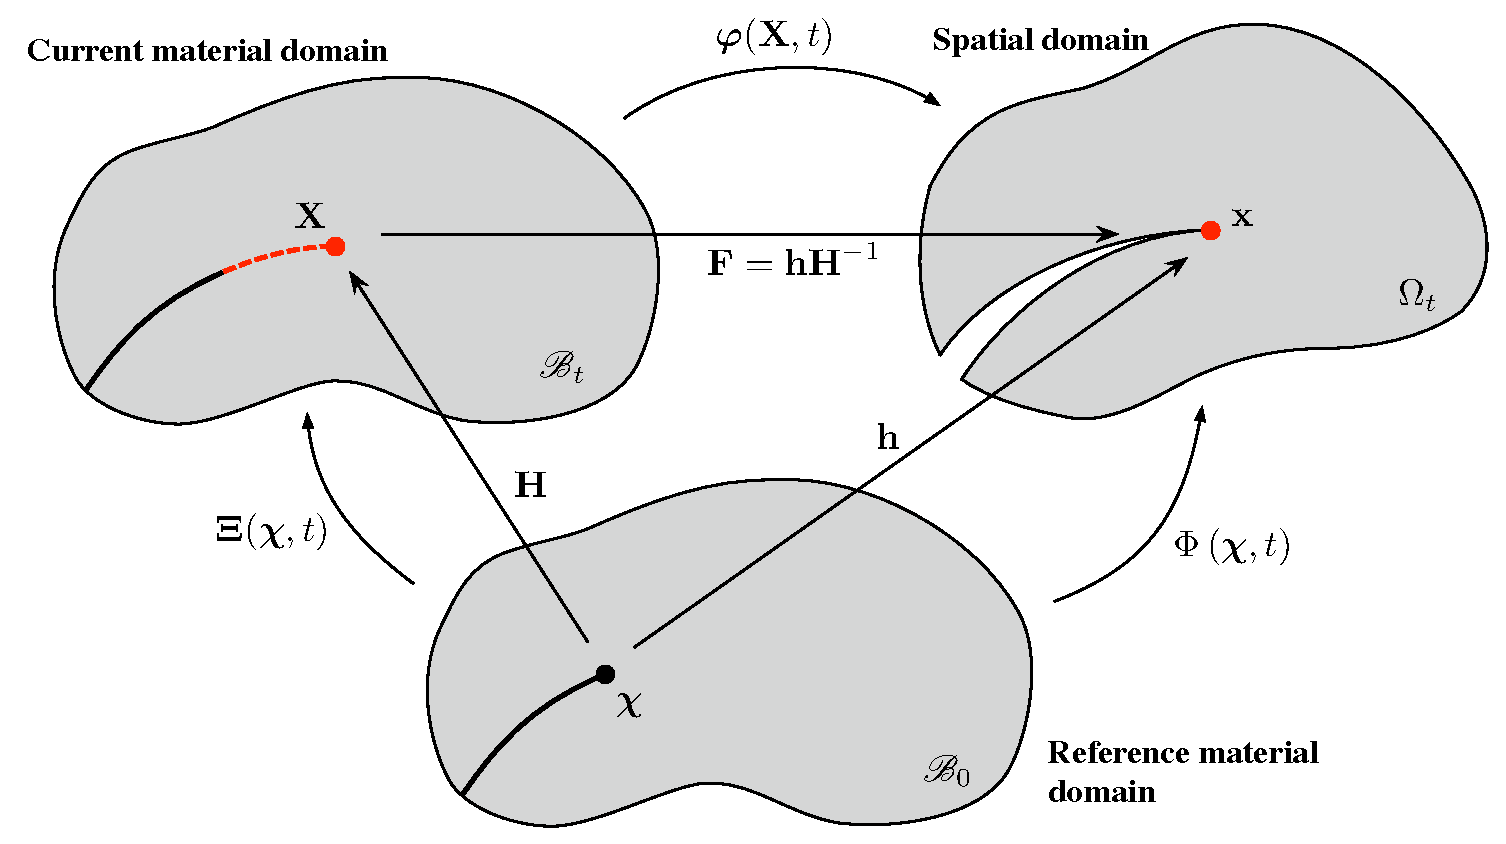
\includegraphics[width=0.7\textwidth]{Figures/domains4.eps} // by Chris (keep as a reference)
%\def\svgwidth{15cm} 	\input{Figures/Configurations.pdf_tex} 
\includegraphics[width=9cm]{Figures/domains5.pdf} 
\end{center}
\caption{Kinematics of crack propagation in elastically deforming body.}
\label{fig:domains4}
\end{figure}

The material coordinates $\mathbf{X}$ are mapped onto the spatial coordinates $\mathbf{x}$ via the
familiar deformation map $\boldsymbol\varphi(\mathbf{X},t)$. The physical displacement is:
\begin{equation}
\mathbf{u}=\mathbf{x}-\mathbf{X}
\end{equation}
The reference material domain describes the body before crack extension. ${\boldsymbol\Xi}(\boldsymbol\chi,t)$ maps the reference material coordinates $\boldsymbol\chi$ on to the current material coordinates $\mathbf{X}$, representing a configurational change, i.e. extension of the crack due to advancement of the crack front. ${\boldsymbol\Phi}$ maps the reference material coordinates $\boldsymbol\chi$ on to the spatial coordinates $\mathbf{x}$. The current material and spatial displacement fields are given as
\begin{equation}
\mathbf{W} = \mathbf{X} - {\boldsymbol\chi}\quad\textrm{and}\quad
\mathbf{w} = \mathbf{x} - {\boldsymbol\chi}
\end{equation}
$\mathbf{H}$ and $\mathbf{h}$ are the gradients of the material and spatial maps and $\mathbf{F}$ is the deformation gradient~\cite{kaczmarczyk2014three}, defined as:
\begin{equation}
\mathbf{H}=\frac{\partial {\boldsymbol\Xi}}{\partial {\boldsymbol\chi}},\quad\mathbf{h}=\frac{\partial {\boldsymbol\Phi}}{\partial {\boldsymbol\chi}},\quad\mathbf{F} = \frac{\partial \boldsymbol\varphi}{\partial \mathbf{X}} = \mathbf{h}\mathbf{H}^{-1}
\end{equation}


The time derivative of the physical displacement $\mathbf{u}$ and the deformation gradient $\mathbf{F}$ (material time derivative) are given as~\cite{kaczmarczyk2014three}:
\begin{equation}\label{eq:phy_vel}
\dot{\mathbf{u}}= \dot{\mathbf{w}}-\mathbf{F}\dot{\mathbf{W}} \qquad 
\dot{\mathbf{F}} = \nabla_\mathbf{X} \dot{\mathbf{x}} = \nabla_\mathbf{X} \dot{\mathbf{u}} = 
\nabla_\mathbf{X} \dot{\mathbf{w}} - \mathbf{F} \nabla_\mathbf{X} \dot{\mathbf{W}}
\end{equation}
 
% \section{Bone adaptation} \label{sec:bone_remodel}
% In this paper, the modelling of bone adaptation is based on the work of Kuhl and Steinmann~\cite{kuhl2003theory} in which bone is considered an elastic porous material. The model is stable~\cite{kuhl2003computational}, efficient~\cite{kaczmarczyk2011efficient} and capable of 
% producing bone mineral density profiles that are quantitatively comparable with DEXA scans following gait analysis~\cite{pang2012computational}. 
% Using this approach, bone adaptation in human scapula~\cite{liedtke2017computational}, 
% tibia~\cite{pang2012computational}, humerus~\cite{taylor2009phenomenon} and femur with various surgical implants~\cite{ambrosi2011perspectives, Connor2017bone} have been simulated and its potential in topology optimization~\cite{waffenschmidt2012application} has been explored. 
% One of the advantages of such a phenomenological approach is that only a small number of parameters are required, which can be experimentally
% determined from, for example, CT imaging~\cite{zadpoor2013open}.


% \subsection{Conservation of mass}

% Following Kuhl and Steinmann~\cite{kuhl2003computational}, it is assumed that
% the rate of change of the time-dependent material density is in equilibrium
% with mass flux, expressed as:
% \begin{equation} \label{eq:mass_balance}
% \frac{\partial\rho}{\partial t}  + \dot{\mathbf{W}} \cdot  \nabla_\mathbf{X} \rho = 
% \nabla_{\boldsymbol {\rm X}} \cdot \mathbf{R} + \mathcal{R}_0
% \end{equation}
% where $\rho$ is mass density and $\mathcal{R}_0$ is the locally created mass.
% It is worth noting that, comparing to Kuhl and Steinmann, we require a material time derivative since the reference material configuration is changing, leading to the addition of the second term in Eq.~\ref{eq:mass_balance}. This is only a kinematic extension of the formulation and does not change the description of the physical problem. 

% Furthermore, $\mathbf{R}$ is the mass flux defined as:
% % 
% \begin{equation}
% \mathbf{R} = \mathcal{R} \nabla_\mathbf{X} \rho
% \label{eq:mass_flux}
% \end{equation}
% % 
% where $\mathcal{R}$ is mass conductivity. The term on the right hand side of Eq. \ref{eq:mass_balance}
% is the material time derivative associated with the evolving current material
% configuration. 
% However, in the present work it is assumed that the mass flux $\mathbf{R}$ is zero and hence only the local mass source $\mathcal{R}_0$ contributes to the changes in density.


% \subsubsection{Constitutive relationship for bone adaptation}

% \label{sec:constitutive_eq}

% In the context of bone mechanics, the constitutive law for the mass source $\mathcal{R}_{0}$ is commonly in the form proposed by Harrigan and Hamilton~\cite{Harrigan1993}. This well established approach has been used e.g. in \citep{harrigan1996bone, taylor2009phenomenon, pang2012computational, hambli2013integrated, kuhl2003computational}. 
% It is assumed that the local increase/decrease in density is governed by the elastic energy as follows:
% \begin{equation}
% \mathcal{R}_{0}=c\left[\Biggl[\frac{\rho}{\rho_{0}^{\ast}}\Biggr]^{-m}\Psi
% -\Psi^{\ast}\right]
% \label{eq:mass_source}
% \end{equation}
% where $\rho_0^\ast$ and $\Psi^\ast$ represent reference values of the
% density, $\rho$ and free energy, $\Psi$, respectively. The driving term
% $\left[ \rho / \rho_0^\ast \right]^{-m}\Psi$ tends to converge to
% $\Psi^\ast$ (see Eq.~(\ref{eq:mass_source})) when density saturation is
% achieved and local generation of bone ceases. The exponent $m$ is a
% dimensionless scalar introduced to guarantee uniqueness and
% stability~\cite{Harrigan1993}. The coefficient $c$ controls
% the rate of the adaptation process with units~$[\rm{s/cm^2}]$. 
% % As proposed in~\cite{Waffenschmidt2012}, it can be beneficial to prescribe an upper and
% % lower bound for bone density, thereby avoiding spurious or non-physical
% % values (lower than zero or greater than observed maximum). In this paper, the parameter $c$, which is conventionally considered 
% % to be constant, is replaced by a bell function
% % defined as:
% % \begin{equation}
% % \begin{aligned}
% % c(\rho) = & \frac{1}{1 + \left[  (\rho - \rho^{\mathrm{mid}}) / 
% % (\rho{^\mathrm{max}} - \rho{^\mathrm{mid})} \right]^{2 b}}\\
% % & \mathrm{with} \quad \rho^{\mathrm{mid}} = 
% % \frac{\rho{^\mathrm{max}} + \rho{^\mathrm{min}}}{2}
% % \end{aligned}
% % \label{eq:bell_function}
% % \end{equation}
% % $\rho^\mathrm{max}$ and $ \rho{^\mathrm{min}}$ where $\rho^\mathrm{max}$
% % and $\rho^\mathrm{min}$ are the maximum and minimum values of $\rho$, and
% % $\rho^{\rm {mid}}$ is their average. The bell function
% % (\ref{eq:bell_function}) is illustrated in Figure~\ref{fig:bell_func} for
% % different values of the integer exponent, $b$. Its application and influence
% % on the overall results are elaborated in
% % Section~\ref{sec:numerical_examples}.
% % \begin{figure}[!htb]
% % 	\centering
% % 		% This file was created by matlab2tikz.
%
%The latest updates can be retrieved from
%  http://www.mathworks.com/matlabcentral/fileexchange/22022-matlab2tikz-matlab2tikz
%where you can also make suggestions and rate matlab2tikz.
%
\definecolor{mycolor1}{rgb}{1.00000,0.00000,1.00000}%
%

\begin{tikzpicture}

\begin{axis}[%
width=9cm,
height=6cm,
at={(0cm,0cm)},
scale only axis,
unbounded coords=jump,
xmin=0,
xmax=8,
xtick={0,2,4,6},
xticklabels={{0},{$\rho^\mathrm{min}$},{$\rho^\mathrm{mid}$},{$\rho^\mathrm{max}$}},
xlabel style={font=\color{white!15!black}},
xlabel={$\rho [\mathrm g / \mathrm{cm}^3]$},
ymin=-0.1,
ymax=1.2,
ylabel style={font=\color{white!15!black}},
ylabel={$c [\mathrm s / \mathrm{cm}^2]$},
axis background/.style={fill=white},
legend style={legend cell align=left, align=left, fill=none, draw=none}
]

\addplot [color=black, line width=2.0pt]
  table[row sep=crcr]{%
0	0.5\\
0.01	0.5\\
0.02	0.5\\
0.03	0.5\\
0.04	0.5\\
0.05	0.5\\
0.06	0.5\\
0.07	0.5\\
0.08	0.5\\
0.09	0.5\\
0.1	0.5\\
0.11	0.5\\
0.12	0.5\\
0.13	0.5\\
0.14	0.5\\
0.15	0.5\\
0.16	0.5\\
0.17	0.5\\
0.18	0.5\\
0.19	0.5\\
0.2	0.5\\
0.21	0.5\\
0.22	0.5\\
0.23	0.5\\
0.24	0.5\\
0.25	0.5\\
0.26	0.5\\
0.27	0.5\\
0.28	0.5\\
0.29	0.5\\
0.3	0.5\\
0.31	0.5\\
0.32	0.5\\
0.33	0.5\\
0.34	0.5\\
0.35	0.5\\
0.36	0.5\\
0.37	0.5\\
0.38	0.5\\
0.39	0.5\\
0.4	0.5\\
0.41	0.5\\
0.42	0.5\\
0.43	0.5\\
0.44	0.5\\
0.45	0.5\\
0.46	0.5\\
0.47	0.5\\
0.48	0.5\\
0.49	0.5\\
0.5	0.5\\
0.51	0.5\\
0.52	0.5\\
0.53	0.5\\
0.54	0.5\\
0.55	0.5\\
0.56	0.5\\
0.57	0.5\\
0.58	0.5\\
0.59	0.5\\
0.6	0.5\\
0.61	0.5\\
0.62	0.5\\
0.63	0.5\\
0.64	0.5\\
0.65	0.5\\
0.66	0.5\\
0.67	0.5\\
0.68	0.5\\
0.69	0.5\\
0.7	0.5\\
0.71	0.5\\
0.72	0.5\\
0.73	0.5\\
0.74	0.5\\
0.75	0.5\\
0.76	0.5\\
0.77	0.5\\
0.78	0.5\\
0.79	0.5\\
0.8	0.5\\
0.81	0.5\\
0.82	0.5\\
0.83	0.5\\
0.84	0.5\\
0.85	0.5\\
0.86	0.5\\
0.87	0.5\\
0.88	0.5\\
0.89	0.5\\
0.9	0.5\\
0.91	0.5\\
0.92	0.5\\
0.93	0.5\\
0.94	0.5\\
0.95	0.5\\
0.96	0.5\\
0.97	0.5\\
0.98	0.5\\
0.99	0.5\\
1	0.5\\
1.01	0.5\\
1.02	0.5\\
1.03	0.5\\
1.04	0.5\\
1.05	0.5\\
1.06	0.5\\
1.07	0.5\\
1.08	0.5\\
1.09	0.5\\
1.1	0.5\\
1.11	0.5\\
1.12	0.5\\
1.13	0.5\\
1.14	0.5\\
1.15	0.5\\
1.16	0.5\\
1.17	0.5\\
1.18	0.5\\
1.19	0.5\\
1.2	0.5\\
1.21	0.5\\
1.22	0.5\\
1.23	0.5\\
1.24	0.5\\
1.25	0.5\\
1.26	0.5\\
1.27	0.5\\
1.28	0.5\\
1.29	0.5\\
1.3	0.5\\
1.31	0.5\\
1.32	0.5\\
1.33	0.5\\
1.34	0.5\\
1.35	0.5\\
1.36	0.5\\
1.37	0.5\\
1.38	0.5\\
1.39	0.5\\
1.4	0.5\\
1.41	0.5\\
1.42	0.5\\
1.43	0.5\\
1.44	0.5\\
1.45	0.5\\
1.46	0.5\\
1.47	0.5\\
1.48	0.5\\
1.49	0.5\\
1.5	0.5\\
1.51	0.5\\
1.52	0.5\\
1.53	0.5\\
1.54	0.5\\
1.55	0.5\\
1.56	0.5\\
1.57	0.5\\
1.58	0.5\\
1.59	0.5\\
1.6	0.5\\
1.61	0.5\\
1.62	0.5\\
1.63	0.5\\
1.64	0.5\\
1.65	0.5\\
1.66	0.5\\
1.67	0.5\\
1.68	0.5\\
1.69	0.5\\
1.7	0.5\\
1.71	0.5\\
1.72	0.5\\
1.73	0.5\\
1.74	0.5\\
1.75	0.5\\
1.76	0.5\\
1.77	0.5\\
1.78	0.5\\
1.79	0.5\\
1.8	0.5\\
1.81	0.5\\
1.82	0.5\\
1.83	0.5\\
1.84	0.5\\
1.85	0.5\\
1.86	0.5\\
1.87	0.5\\
1.88	0.5\\
1.89	0.5\\
1.9	0.5\\
1.91	0.5\\
1.92	0.5\\
1.93	0.5\\
1.94	0.5\\
1.95	0.5\\
1.96	0.5\\
1.97	0.5\\
1.98	0.5\\
1.99	0.5\\
2	0.5\\
2.01	0.5\\
2.02	0.5\\
2.03	0.5\\
2.04	0.5\\
2.05	0.5\\
2.06	0.5\\
2.07	0.5\\
2.08	0.5\\
2.09	0.5\\
2.1	0.5\\
2.11	0.5\\
2.12	0.5\\
2.13	0.5\\
2.14	0.5\\
2.15	0.5\\
2.16	0.5\\
2.17	0.5\\
2.18	0.5\\
2.19	0.5\\
2.2	0.5\\
2.21	0.5\\
2.22	0.5\\
2.23	0.5\\
2.24	0.5\\
2.25	0.5\\
2.26	0.5\\
2.27	0.5\\
2.28	0.5\\
2.29	0.5\\
2.3	0.5\\
2.31	0.5\\
2.32	0.5\\
2.33	0.5\\
2.34	0.5\\
2.35	0.5\\
2.36	0.5\\
2.37	0.5\\
2.38	0.5\\
2.39	0.5\\
2.4	0.5\\
2.41	0.5\\
2.42	0.5\\
2.43	0.5\\
2.44	0.5\\
2.45	0.5\\
2.46	0.5\\
2.47	0.5\\
2.48	0.5\\
2.49	0.5\\
2.5	0.5\\
2.51	0.5\\
2.52	0.5\\
2.53	0.5\\
2.54	0.5\\
2.55	0.5\\
2.56	0.5\\
2.57	0.5\\
2.58	0.5\\
2.59	0.5\\
2.6	0.5\\
2.61	0.5\\
2.62	0.5\\
2.63	0.5\\
2.64	0.5\\
2.65	0.5\\
2.66	0.5\\
2.67	0.5\\
2.68	0.5\\
2.69	0.5\\
2.7	0.5\\
2.71	0.5\\
2.72	0.5\\
2.73	0.5\\
2.74	0.5\\
2.75	0.5\\
2.76	0.5\\
2.77	0.5\\
2.78	0.5\\
2.79	0.5\\
2.8	0.5\\
2.81	0.5\\
2.82	0.5\\
2.83	0.5\\
2.84	0.5\\
2.85	0.5\\
2.86	0.5\\
2.87	0.5\\
2.88	0.5\\
2.89	0.5\\
2.9	0.5\\
2.91	0.5\\
2.92	0.5\\
2.93	0.5\\
2.94	0.5\\
2.95	0.5\\
2.96	0.5\\
2.97	0.5\\
2.98	0.5\\
2.99	0.5\\
3	0.5\\
3.01	0.5\\
3.02	0.5\\
3.03	0.5\\
3.04	0.5\\
3.05	0.5\\
3.06	0.5\\
3.07	0.5\\
3.08	0.5\\
3.09	0.5\\
3.1	0.5\\
3.11	0.5\\
3.12	0.5\\
3.13	0.5\\
3.14	0.5\\
3.15	0.5\\
3.16	0.5\\
3.17	0.5\\
3.18	0.5\\
3.19	0.5\\
3.2	0.5\\
3.21	0.5\\
3.22	0.5\\
3.23	0.5\\
3.24	0.5\\
3.25	0.5\\
3.26	0.5\\
3.27	0.5\\
3.28	0.5\\
3.29	0.5\\
3.3	0.5\\
3.31	0.5\\
3.32	0.5\\
3.33	0.5\\
3.34	0.5\\
3.35	0.5\\
3.36	0.5\\
3.37	0.5\\
3.38	0.5\\
3.39	0.5\\
3.4	0.5\\
3.41	0.5\\
3.42	0.5\\
3.43	0.5\\
3.44	0.5\\
3.45	0.5\\
3.46	0.5\\
3.47	0.5\\
3.48	0.5\\
3.49	0.5\\
3.5	0.5\\
3.51	0.5\\
3.52	0.5\\
3.53	0.5\\
3.54	0.5\\
3.55	0.5\\
3.56	0.5\\
3.57	0.5\\
3.58	0.5\\
3.59	0.5\\
3.6	0.5\\
3.61	0.5\\
3.62	0.5\\
3.63	0.5\\
3.64	0.5\\
3.65	0.5\\
3.66	0.5\\
3.67	0.5\\
3.68	0.5\\
3.69	0.5\\
3.7	0.5\\
3.71	0.5\\
3.72	0.5\\
3.73	0.5\\
3.74	0.5\\
3.75	0.5\\
3.76	0.5\\
3.77	0.5\\
3.78	0.5\\
3.79	0.5\\
3.8	0.5\\
3.81	0.5\\
3.82	0.5\\
3.83	0.5\\
3.84	0.5\\
3.85	0.5\\
3.86	0.5\\
3.87	0.5\\
3.88	0.5\\
3.89	0.5\\
3.9	0.5\\
3.91	0.5\\
3.92	0.5\\
3.93	0.5\\
3.94	0.5\\
3.95	0.5\\
3.96	0.5\\
3.97	0.5\\
3.98	0.5\\
3.99	0.5\\
4	0.5\\
4.01	0.5\\
4.02	0.5\\
4.03	0.5\\
4.04	0.5\\
4.05	0.5\\
4.06	0.5\\
4.07	0.5\\
4.08	0.5\\
4.09	0.5\\
4.1	0.5\\
4.11	0.5\\
4.12	0.5\\
4.13	0.5\\
4.14	0.5\\
4.15	0.5\\
4.16	0.5\\
4.17	0.5\\
4.18	0.5\\
4.19	0.5\\
4.2	0.5\\
4.21	0.5\\
4.22	0.5\\
4.23	0.5\\
4.24	0.5\\
4.25	0.5\\
4.26	0.5\\
4.27	0.5\\
4.28	0.5\\
4.29	0.5\\
4.3	0.5\\
4.31	0.5\\
4.32	0.5\\
4.33	0.5\\
4.34	0.5\\
4.35	0.5\\
4.36	0.5\\
4.37	0.5\\
4.38	0.5\\
4.39	0.5\\
4.4	0.5\\
4.41	0.5\\
4.42	0.5\\
4.43	0.5\\
4.44	0.5\\
4.45	0.5\\
4.46	0.5\\
4.47	0.5\\
4.48	0.5\\
4.49	0.5\\
4.5	0.5\\
4.51	0.5\\
4.52	0.5\\
4.53	0.5\\
4.54	0.5\\
4.55	0.5\\
4.56	0.5\\
4.57	0.5\\
4.58	0.5\\
4.59	0.5\\
4.6	0.5\\
4.61	0.5\\
4.62	0.5\\
4.63	0.5\\
4.64	0.5\\
4.65	0.5\\
4.66	0.5\\
4.67	0.5\\
4.68	0.5\\
4.69	0.5\\
4.7	0.5\\
4.71	0.5\\
4.72	0.5\\
4.73	0.5\\
4.74	0.5\\
4.75	0.5\\
4.76	0.5\\
4.77	0.5\\
4.78	0.5\\
4.79	0.5\\
4.8	0.5\\
4.81	0.5\\
4.82	0.5\\
4.83	0.5\\
4.84	0.5\\
4.85	0.5\\
4.86	0.5\\
4.87	0.5\\
4.88	0.5\\
4.89	0.5\\
4.9	0.5\\
4.91	0.5\\
4.92	0.5\\
4.93	0.5\\
4.94	0.5\\
4.95	0.5\\
4.96	0.5\\
4.97	0.5\\
4.98	0.5\\
4.99	0.5\\
5	0.5\\
5.01	0.5\\
5.02	0.5\\
5.03	0.5\\
5.04	0.5\\
5.05	0.5\\
5.06	0.5\\
5.07	0.5\\
5.08	0.5\\
5.09	0.5\\
5.1	0.5\\
5.11	0.5\\
5.12	0.5\\
5.13	0.5\\
5.14	0.5\\
5.15	0.5\\
5.16	0.5\\
5.17	0.5\\
5.18	0.5\\
5.19	0.5\\
5.2	0.5\\
5.21	0.5\\
5.22	0.5\\
5.23	0.5\\
5.24	0.5\\
5.25	0.5\\
5.26	0.5\\
5.27	0.5\\
5.28	0.5\\
5.29	0.5\\
5.3	0.5\\
5.31	0.5\\
5.32	0.5\\
5.33	0.5\\
5.34	0.5\\
5.35	0.5\\
5.36	0.5\\
5.37	0.5\\
5.38	0.5\\
5.39	0.5\\
5.4	0.5\\
5.41	0.5\\
5.42	0.5\\
5.43	0.5\\
5.44	0.5\\
5.45	0.5\\
5.46	0.5\\
5.47	0.5\\
5.48	0.5\\
5.49	0.5\\
5.5	0.5\\
5.51	0.5\\
5.52	0.5\\
5.53	0.5\\
5.54	0.5\\
5.55	0.5\\
5.56	0.5\\
5.57	0.5\\
5.58	0.5\\
5.59	0.5\\
5.6	0.5\\
5.61	0.5\\
5.62	0.5\\
5.63	0.5\\
5.64	0.5\\
5.65	0.5\\
5.66	0.5\\
5.67	0.5\\
5.68	0.5\\
5.69	0.5\\
5.7	0.5\\
5.71	0.5\\
5.72	0.5\\
5.73	0.5\\
5.74	0.5\\
5.75	0.5\\
5.76	0.5\\
5.77	0.5\\
5.78	0.5\\
5.79	0.5\\
5.8	0.5\\
5.81	0.5\\
5.82	0.5\\
5.83	0.5\\
5.84	0.5\\
5.85	0.5\\
5.86	0.5\\
5.87	0.5\\
5.88	0.5\\
5.89	0.5\\
5.9	0.5\\
5.91	0.5\\
5.92	0.5\\
5.93	0.5\\
5.94	0.5\\
5.95	0.5\\
5.96	0.5\\
5.97	0.5\\
5.98	0.5\\
5.99	0.5\\
6	0.5\\
6.01	0.5\\
6.02	0.5\\
6.03	0.5\\
6.04	0.5\\
6.05	0.5\\
6.06	0.5\\
6.07	0.5\\
6.08	0.5\\
6.09	0.5\\
6.1	0.5\\
6.11	0.5\\
6.12	0.5\\
6.13	0.5\\
6.14	0.5\\
6.15	0.5\\
6.16	0.5\\
6.17	0.5\\
6.18	0.5\\
6.19	0.5\\
6.2	0.5\\
6.21	0.5\\
6.22	0.5\\
6.23	0.5\\
6.24	0.5\\
6.25	0.5\\
6.26	0.5\\
6.27	0.5\\
6.28	0.5\\
6.29	0.5\\
6.3	0.5\\
6.31	0.5\\
6.32	0.5\\
6.33	0.5\\
6.34	0.5\\
6.35	0.5\\
6.36	0.5\\
6.37	0.5\\
6.38	0.5\\
6.39	0.5\\
6.4	0.5\\
6.41	0.5\\
6.42	0.5\\
6.43	0.5\\
6.44	0.5\\
6.45	0.5\\
6.46	0.5\\
6.47	0.5\\
6.48	0.5\\
6.49	0.5\\
6.5	0.5\\
6.51	0.5\\
6.52	0.5\\
6.53	0.5\\
6.54	0.5\\
6.55	0.5\\
6.56	0.5\\
6.57	0.5\\
6.58	0.5\\
6.59	0.5\\
6.6	0.5\\
6.61	0.5\\
6.62	0.5\\
6.63	0.5\\
6.64	0.5\\
6.65	0.5\\
6.66	0.5\\
6.67	0.5\\
6.68	0.5\\
6.69	0.5\\
6.7	0.5\\
6.71	0.5\\
6.72	0.5\\
6.73	0.5\\
6.74	0.5\\
6.75	0.5\\
6.76	0.5\\
6.77	0.5\\
6.78	0.5\\
6.79	0.5\\
6.8	0.5\\
6.81	0.5\\
6.82	0.5\\
6.83	0.5\\
6.84	0.5\\
6.85	0.5\\
6.86	0.5\\
6.87	0.5\\
6.88	0.5\\
6.89	0.5\\
6.9	0.5\\
6.91	0.5\\
6.92	0.5\\
6.93	0.5\\
6.94	0.5\\
6.95	0.5\\
6.96	0.5\\
6.97	0.5\\
6.98	0.5\\
6.99	0.5\\
7	0.5\\
7.01	0.5\\
7.02	0.5\\
7.03	0.5\\
7.04	0.5\\
7.05	0.5\\
7.06	0.5\\
7.07	0.5\\
7.08	0.5\\
7.09	0.5\\
7.1	0.5\\
7.11	0.5\\
7.12	0.5\\
7.13	0.5\\
7.14	0.5\\
7.15	0.5\\
7.16	0.5\\
7.17	0.5\\
7.18	0.5\\
7.19	0.5\\
7.2	0.5\\
7.21	0.5\\
7.22	0.5\\
7.23	0.5\\
7.24	0.5\\
7.25	0.5\\
7.26	0.5\\
7.27	0.5\\
7.28	0.5\\
7.29	0.5\\
7.3	0.5\\
7.31	0.5\\
7.32	0.5\\
7.33	0.5\\
7.34	0.5\\
7.35	0.5\\
7.36	0.5\\
7.37	0.5\\
7.38	0.5\\
7.39	0.5\\
7.4	0.5\\
7.41	0.5\\
7.42	0.5\\
7.43	0.5\\
7.44	0.5\\
7.45	0.5\\
7.46	0.5\\
7.47	0.5\\
7.48	0.5\\
7.49	0.5\\
7.5	0.5\\
7.51	0.5\\
7.52	0.5\\
7.53	0.5\\
7.54	0.5\\
7.55	0.5\\
7.56	0.5\\
7.57	0.5\\
7.58	0.5\\
7.59	0.5\\
7.6	0.5\\
7.61	0.5\\
7.62	0.5\\
7.63	0.5\\
7.64	0.5\\
7.65	0.5\\
7.66	0.5\\
7.67	0.5\\
7.68	0.5\\
7.69	0.5\\
7.7	0.5\\
7.71	0.5\\
7.72	0.5\\
7.73	0.5\\
7.74	0.5\\
7.75	0.5\\
7.76	0.5\\
7.77	0.5\\
7.78	0.5\\
7.79	0.5\\
7.8	0.5\\
7.81	0.5\\
7.82	0.5\\
7.83	0.5\\
7.84	0.5\\
7.85	0.5\\
7.86	0.5\\
7.87	0.5\\
7.88	0.5\\
7.89	0.5\\
7.9	0.5\\
7.91	0.5\\
7.92	0.5\\
7.93	0.5\\
7.94	0.5\\
7.95	0.5\\
7.96	0.5\\
7.97	0.5\\
7.98	0.5\\
7.99	0.5\\
8	0.5\\
};
\addplot [color=black, line width=2.0pt]
  table[row sep=crcr]{%
nan	nan\\
};
\addlegendentry{$b=0$}

\addplot [color=green, dashed, line width=2.0pt]
  table[row sep=crcr]{%
0	0.2\\
0.01	0.200802204808209\\
0.02	0.201608838531481\\
0.03	0.202419930266334\\
0.04	0.203235509308186\\
0.05	0.204055605152404\\
0.06	0.204880247495339\\
0.07	0.205709466235362\\
0.08	0.206543291473893\\
0.09	0.207381753516417\\
0.1	0.208224882873503\\
0.11	0.209072710261811\\
0.12	0.209925266605089\\
0.13	0.210782583035164\\
0.14	0.211644690892929\\
0.15	0.212511621729313\\
0.16	0.213383407306248\\
0.17	0.21426007959762\\
0.18	0.215141670790215\\
0.19	0.216028213284655\\
0.2	0.216919739696312\\
0.21	0.217816282856225\\
0.22	0.21871787581199\\
0.23	0.219624551828649\\
0.24	0.220536344389555\\
0.25	0.221453287197232\\
0.26	0.222375414174209\\
0.27	0.22330275946385\\
0.28	0.22423535743116\\
0.29	0.225173242663574\\
0.3	0.226116449971735\\
0.31	0.227065014390245\\
0.32	0.228018971178402\\
0.33	0.228978355820916\\
0.34	0.229943204028605\\
0.35	0.230913551739068\\
0.36	0.231889435117336\\
0.37	0.232870890556503\\
0.38	0.233857954678328\\
0.39	0.234850664333817\\
0.4	0.235849056603774\\
0.41	0.236853168799332\\
0.42	0.237863038462453\\
0.43	0.238878703366398\\
0.44	0.239900201516169\\
0.45	0.240927571148923\\
0.46	0.241960850734351\\
0.47	0.243000078975026\\
0.48	0.244045294806716\\
0.49	0.245096537398668\\
0.5	0.246153846153846\\
0.51	0.247217260709143\\
0.52	0.248286820935545\\
0.53	0.249362566938264\\
0.54	0.250444539056826\\
0.55	0.251532777865116\\
0.56	0.252627324171382\\
0.57	0.253728219018199\\
0.58	0.254835503682373\\
0.59	0.255949219674816\\
0.6	0.25706940874036\\
0.61	0.258196112857521\\
0.62	0.25932937423822\\
0.63	0.260469235327442\\
0.64	0.261615738802846\\
0.65	0.262768927574314\\
0.66	0.263928844783446\\
0.67	0.265095533802994\\
0.68	0.266269038236234\\
0.69	0.267449401916275\\
0.7	0.268636668905306\\
0.71	0.26983088349377\\
0.72	0.27103209019948\\
0.73	0.272240333766649\\
0.74	0.273455659164866\\
0.75	0.274678111587983\\
0.76	0.27590773645293\\
0.77	0.277144579398458\\
0.78	0.278388686283789\\
0.79	0.279640103187198\\
0.8	0.280898876404494\\
0.81	0.282165052447429\\
0.82	0.283438678042006\\
0.83	0.2847198001267\\
0.84	0.286008465850589\\
0.85	0.287304722571377\\
0.86	0.288608617853329\\
0.87	0.289920199465097\\
0.88	0.291239515377446\\
0.89	0.292566613760871\\
0.9	0.293901542983101\\
0.91	0.295244351606498\\
0.92	0.296595088385336\\
0.93	0.297953802262959\\
0.94	0.299320542368823\\
0.95	0.300695358015411\\
0.96	0.302078298695022\\
0.97	0.303469414076429\\
0.98	0.304868754001402\\
0.99	0.306276368481099\\
1	0.307692307692308\\
1.01	0.309116621973555\\
1.02	0.310549361821061\\
1.03	0.311990577884548\\
1.04	0.313440320962889\\
1.05	0.314898641999606\\
1.06	0.316365592078206\\
1.07	0.317841222417341\\
1.08	0.319325584365819\\
1.09	0.320818729397422\\
1.1	0.32232070910556\\
1.11	0.32383157519774\\
1.12	0.325351379489849\\
1.13	0.326880173900252\\
1.14	0.328418010443693\\
1.15	0.329964941224995\\
1.16	0.331521018432569\\
1.17	0.333086294331704\\
1.18	0.334660821257655\\
1.19	0.33624465160851\\
1.2	0.337837837837838\\
1.21	0.339440432447111\\
1.22	0.3410524879779\\
1.23	0.342674057003829\\
1.24	0.344305192122297\\
1.25	0.345945945945946\\
1.26	0.347596371093886\\
1.27	0.349256520182661\\
1.28	0.350926445816957\\
1.29	0.352606200580037\\
1.3	0.354295837023915\\
1.31	0.355995407659241\\
1.32	0.357704964944913\\
1.33	0.359424561277395\\
1.34	0.361154248979739\\
1.35	0.362894080290315\\
1.36	0.364644107351225\\
1.37	0.366404382196411\\
1.38	0.368174956739443\\
1.39	0.369955882760981\\
1.4	0.371747211895911\\
1.41	0.373548995620138\\
1.42	0.375361285237041\\
1.43	0.377184131863572\\
1.44	0.37901758641601\\
1.45	0.380861699595334\\
1.46	0.382716521872249\\
1.47	0.384582103471815\\
1.48	0.386458494357706\\
1.49	0.388345744216076\\
1.5	0.390243902439024\\
1.51	0.392153018107666\\
1.52	0.394073139974779\\
1.53	0.396004316447049\\
1.54	0.397946595566875\\
1.55	0.399900024993751\\
1.56	0.401864651985211\\
1.57	0.403840523377318\\
1.58	0.405827685564709\\
1.59	0.407826184480175\\
1.6	0.409836065573771\\
1.61	0.411857373791456\\
1.62	0.413890153553247\\
1.63	0.41593444873088\\
1.64	0.417990302624979\\
1.65	0.420057757941717\\
1.66	0.422136856768965\\
1.67	0.42422764055192\\
1.68	0.426330150068213\\
1.69	0.42844442540247\\
1.7	0.430570505920345\\
1.71	0.432708430241992\\
1.72	0.434858236214994\\
1.73	0.437019960886714\\
1.74	0.439193640476086\\
1.75	0.441379310344828\\
1.76	0.443577004968062\\
1.77	0.445786757904357\\
1.78	0.448008601765154\\
1.79	0.450242568183609\\
1.8	0.452488687782805\\
1.81	0.454746990143359\\
1.82	0.457017503770395\\
1.83	0.459300256059893\\
1.84	0.461595273264402\\
1.85	0.463902580458104\\
1.86	0.466222201501236\\
1.87	0.468554159003854\\
1.88	0.470898474288943\\
1.89	0.473255167354859\\
1.9	0.475624256837099\\
1.91	0.478005759969408\\
1.92	0.480399692544197\\
1.93	0.482806068872286\\
1.94	0.485224901741957\\
1.95	0.487656202377324\\
1.96	0.490099980396001\\
1.97	0.492556243766085\\
1.98	0.495024998762437\\
1.99	0.497506249922265\\
2	0.5\\
2.01	0.502506249921484\\
2.02	0.505024998737438\\
2.03	0.507556243576241\\
2.04	0.510099979596001\\
2.05	0.512656199935918\\
2.06	0.515224895666959\\
2.07	0.517806055741822\\
2.08	0.520399666944213\\
2.09	0.523005713837424\\
2.1	0.525624178712221\\
2.11	0.528255041534053\\
2.12	0.530898279889573\\
2.13	0.533553868932492\\
2.14	0.536221781328758\\
2.15	0.538901987201078\\
2.16	0.54159445407279\\
2.17	0.544299146811087\\
2.18	0.547016027569608\\
2.19	0.549745055730405\\
2.2	0.552486187845304\\
2.21	0.555239377576658\\
2.22	0.55800457563752\\
2.23	0.560781729731245\\
2.24	0.563570784490532\\
2.25	0.566371681415929\\
2.26	0.56918435881382\\
2.27	0.572008751733902\\
2.28	0.574844791906185\\
2.29	0.577692407677532\\
2.3	0.58055152394775\\
2.31	0.583422062105279\\
2.32	0.586303939962477\\
2.33	0.589197071690554\\
2.34	0.592101367754159\\
2.35	0.595016734845668\\
2.36	0.597943075819182\\
2.37	0.6008802896243\\
2.38	0.603828271239659\\
2.39	0.606786911606317\\
2.4	0.609756097560976\\
2.41	0.612735711769121\\
2.42	0.615725632658088\\
2.43	0.618725734350106\\
2.44	0.621735886595374\\
2.45	0.624755954705193\\
2.46	0.627785799485216\\
2.47	0.630825277168856\\
2.48	0.633874239350913\\
2.49	0.63693253292145\\
2.5	0.64\\
2.51	0.643076477870131\\
2.52	0.646161798914448\\
2.53	0.649255790550082\\
2.54	0.65235827516472\\
2.55	0.655469070053257\\
2.56	0.658587987355111\\
2.57	0.661714833992291\\
2.58	0.664849411608271\\
2.59	0.66799151650774\\
2.6	0.671140939597315\\
2.61	0.67429746632727\\
2.62	0.677460876634374\\
2.63	0.680630944885909\\
2.64	0.683807439824945\\
2.65	0.68699012451696\\
2.66	0.690178756297881\\
2.67	0.693373086723639\\
2.68	0.696572861521315\\
2.69	0.699777820541978\\
2.7	0.70298769771529\\
2.71	0.706202221005985\\
2.72	0.709421112372304\\
2.73	0.712644087726487\\
2.74	0.715870856897416\\
2.75	0.719101123595506\\
2.76	0.722334585379948\\
2.77	0.725570933628399\\
2.78	0.72880985350922\\
2.79	0.73205102395637\\
2.8	0.735294117647059\\
2.81	0.738538800982257\\
2.82	0.741784734070173\\
2.83	0.745031570712809\\
2.84	0.74827895839569\\
2.85	0.751526538280883\\
2.86	0.754773945203412\\
2.87	0.758020807671171\\
2.88	0.761266747868453\\
2.89	0.764511381663195\\
2.9	0.767754318618042\\
2.91	0.770995162005358\\
2.92	0.774233508826262\\
2.93	0.777468949833816\\
2.94	0.780701069560465\\
2.95	0.783929446349829\\
2.96	0.787153652392947\\
2.97	0.790373253769093\\
2.98	0.793587810491231\\
2.99	0.796796876556244\\
3	0.8\\
3.01	0.80319672295737\\
3.02	0.80638658172728\\
3.03	0.809569106842883\\
3.04	0.812743823146944\\
3.05	0.815910249872514\\
3.06	0.819067900728971\\
3.07	0.822216283993505\\
3.08	0.825354902608121\\
3.09	0.828483254282223\\
3.1	0.831600831600832\\
3.11	0.83470712213852\\
3.12	0.837801608579088\\
3.13	0.840883768841052\\
3.14	0.843953076208963\\
3.15	0.847008999470619\\
3.16	0.850051003060184\\
3.17	0.853078547207234\\
3.18	0.856091088091773\\
3.19	0.859088078005197\\
3.2	0.862068965517241\\
3.21	0.865033195648883\\
3.22	0.867980210051211\\
3.23	0.870909447190228\\
3.24	0.873820342537574\\
3.25	0.876712328767123\\
3.26	0.879584835957428\\
3.27	0.882437291799952\\
3.28	0.885269121813031\\
3.29	0.888079749561511\\
3.3	0.89086859688196\\
3.31	0.893635084113402\\
3.32	0.896378630333453\\
3.33	0.899098653599766\\
3.34	0.901794571196681\\
3.35	0.904465799886942\\
3.36	0.90711175616836\\
3.37	0.909731856535286\\
3.38	0.912325517744731\\
3.39	0.914892157086983\\
3.4	0.91743119266055\\
3.41	0.91994204365125\\
3.42	0.922424130615257\\
3.43	0.924876875765914\\
3.44	0.927299703264095\\
3.45	0.929692039511912\\
3.46	0.932053313449529\\
3.47	0.934382956854867\\
3.48	0.936680404645935\\
3.49	0.938945095185559\\
3.5	0.941176470588235\\
3.51	0.943373977028844\\
3.52	0.94553706505295\\
3.53	0.947665189888413\\
3.54	0.949757811758002\\
3.55	0.951814396192742\\
3.56	0.95383441434567\\
3.57	0.955817343305694\\
3.58	0.957762666411263\\
3.59	0.959669873563494\\
3.6	0.961538461538461\\
3.61	0.963367934298307\\
3.62	0.96515780330084\\
3.63	0.966907587807295\\
3.64	0.968616815187912\\
3.65	0.970285021224985\\
3.66	0.971911750413063\\
3.67	0.973496556255932\\
3.68	0.975039001560062\\
3.69	0.976538658724152\\
3.7	0.97799511002445\\
3.71	0.979407947895497\\
3.72	0.980776775205963\\
3.73	0.98210120552923\\
3.74	0.983380863408398\\
3.75	0.984615384615385\\
3.76	0.985804416403785\\
3.77	0.986947617755188\\
3.78	0.988044659618615\\
3.79	0.989095225142801\\
3.8	0.99009900990099\\
3.81	0.991055722107975\\
3.82	0.991965082829084\\
3.83	0.992826826180843\\
3.84	0.993640699523052\\
3.85	0.994406463642014\\
3.86	0.995123892924669\\
3.87	0.995792775523414\\
3.88	0.996412913511359\\
3.89	0.996984123027841\\
3.9	0.997506234413965\\
3.91	0.997979092338016\\
3.92	0.998402555910543\\
3.93	0.998776498788983\\
3.94	0.999100809271656\\
3.95	0.999375390381012\\
3.96	0.999600159936026\\
3.97	0.999775050613612\\
3.98	0.999900009999\\
3.99	0.999975000624984\\
4	1\\
4.01	0.999975000624984\\
4.02	0.999900009999\\
4.03	0.999775050613612\\
4.04	0.999600159936026\\
4.05	0.999375390381012\\
4.06	0.999100809271655\\
4.07	0.998776498788983\\
4.08	0.998402555910543\\
4.09	0.997979092338016\\
4.1	0.997506234413965\\
4.11	0.996984123027841\\
4.12	0.996412913511359\\
4.13	0.995792775523414\\
4.14	0.995123892924669\\
4.15	0.994406463642014\\
4.16	0.993640699523052\\
4.17	0.992826826180843\\
4.18	0.991965082829084\\
4.19	0.991055722107975\\
4.2	0.99009900990099\\
4.21	0.989095225142801\\
4.22	0.988044659618615\\
4.23	0.986947617755188\\
4.24	0.985804416403785\\
4.25	0.984615384615385\\
4.26	0.983380863408398\\
4.27	0.98210120552923\\
4.28	0.980776775205963\\
4.29	0.979407947895497\\
4.3	0.97799511002445\\
4.31	0.976538658724152\\
4.32	0.975039001560062\\
4.33	0.973496556255932\\
4.34	0.971911750413063\\
4.35	0.970285021224985\\
4.36	0.968616815187912\\
4.37	0.966907587807295\\
4.38	0.96515780330084\\
4.39	0.963367934298307\\
4.4	0.961538461538461\\
4.41	0.959669873563494\\
4.42	0.957762666411263\\
4.43	0.955817343305694\\
4.44	0.95383441434567\\
4.45	0.951814396192742\\
4.46	0.949757811758002\\
4.47	0.947665189888413\\
4.48	0.94553706505295\\
4.49	0.943373977028844\\
4.5	0.941176470588235\\
4.51	0.938945095185559\\
4.52	0.936680404645935\\
4.53	0.934382956854867\\
4.54	0.932053313449529\\
4.55	0.929692039511912\\
4.56	0.927299703264095\\
4.57	0.924876875765914\\
4.58	0.922424130615257\\
4.59	0.91994204365125\\
4.6	0.917431192660551\\
4.61	0.914892157086983\\
4.62	0.912325517744731\\
4.63	0.909731856535286\\
4.64	0.90711175616836\\
4.65	0.904465799886942\\
4.66	0.901794571196681\\
4.67	0.899098653599766\\
4.68	0.896378630333453\\
4.69	0.893635084113403\\
4.7	0.89086859688196\\
4.71	0.888079749561511\\
4.72	0.885269121813031\\
4.73	0.882437291799951\\
4.74	0.879584835957428\\
4.75	0.876712328767123\\
4.76	0.873820342537574\\
4.77	0.870909447190229\\
4.78	0.867980210051211\\
4.79	0.865033195648883\\
4.8	0.862068965517241\\
4.81	0.859088078005197\\
4.82	0.856091088091773\\
4.83	0.853078547207234\\
4.84	0.850051003060184\\
4.85	0.847008999470619\\
4.86	0.843953076208963\\
4.87	0.840883768841052\\
4.88	0.837801608579088\\
4.89	0.834707122138519\\
4.9	0.831600831600832\\
4.91	0.828483254282223\\
4.92	0.825354902608121\\
4.93	0.822216283993505\\
4.94	0.819067900728971\\
4.95	0.815910249872514\\
4.96	0.812743823146944\\
4.97	0.809569106842883\\
4.98	0.80638658172728\\
4.99	0.80319672295737\\
5	0.8\\
5.01	0.796796876556244\\
5.02	0.793587810491231\\
5.03	0.790373253769093\\
5.04	0.787153652392947\\
5.05	0.783929446349829\\
5.06	0.780701069560465\\
5.07	0.777468949833816\\
5.08	0.774233508826262\\
5.09	0.770995162005358\\
5.1	0.767754318618042\\
5.11	0.764511381663195\\
5.12	0.761266747868453\\
5.13	0.758020807671171\\
5.14	0.754773945203411\\
5.15	0.751526538280883\\
5.16	0.74827895839569\\
5.17	0.745031570712809\\
5.18	0.741784734070173\\
5.19	0.738538800982257\\
5.2	0.735294117647059\\
5.21	0.73205102395637\\
5.22	0.72880985350922\\
5.23	0.725570933628399\\
5.24	0.722334585379948\\
5.25	0.719101123595506\\
5.26	0.715870856897416\\
5.27	0.712644087726487\\
5.28	0.709421112372304\\
5.29	0.706202221005985\\
5.3	0.70298769771529\\
5.31	0.699777820541978\\
5.32	0.696572861521315\\
5.33	0.693373086723639\\
5.34	0.690178756297881\\
5.35	0.68699012451696\\
5.36	0.683807439824945\\
5.37	0.680630944885909\\
5.38	0.677460876634374\\
5.39	0.67429746632727\\
5.4	0.671140939597315\\
5.41	0.66799151650774\\
5.42	0.664849411608271\\
5.43	0.661714833992291\\
5.44	0.658587987355111\\
5.45	0.655469070053257\\
5.46	0.65235827516472\\
5.47	0.649255790550082\\
5.48	0.646161798914448\\
5.49	0.643076477870131\\
5.5	0.64\\
5.51	0.63693253292145\\
5.52	0.633874239350913\\
5.53	0.630825277168856\\
5.54	0.627785799485216\\
5.55	0.624755954705193\\
5.56	0.621735886595374\\
5.57	0.618725734350106\\
5.58	0.615725632658088\\
5.59	0.612735711769121\\
5.6	0.609756097560976\\
5.61	0.606786911606317\\
5.62	0.603828271239659\\
5.63	0.6008802896243\\
5.64	0.597943075819182\\
5.65	0.595016734845667\\
5.66	0.592101367754159\\
5.67	0.589197071690554\\
5.68	0.586303939962477\\
5.69	0.583422062105279\\
5.7	0.580551523947751\\
5.71	0.577692407677532\\
5.72	0.574844791906185\\
5.73	0.572008751733901\\
5.74	0.56918435881382\\
5.75	0.566371681415929\\
5.76	0.563570784490532\\
5.77	0.560781729731246\\
5.78	0.55800457563752\\
5.79	0.555239377576658\\
5.8	0.552486187845304\\
5.81	0.549745055730405\\
5.82	0.547016027569608\\
5.83	0.544299146811087\\
5.84	0.54159445407279\\
5.85	0.538901987201078\\
5.86	0.536221781328758\\
5.87	0.533553868932492\\
5.88	0.530898279889573\\
5.89	0.528255041534052\\
5.9	0.525624178712221\\
5.91	0.523005713837424\\
5.92	0.520399666944213\\
5.93	0.517806055741822\\
5.94	0.515224895666959\\
5.95	0.512656199935918\\
5.96	0.510099979596001\\
5.97	0.507556243576241\\
5.98	0.505024998737437\\
5.99	0.502506249921483\\
6	0.5\\
6.01	0.497506249922265\\
6.02	0.495024998762438\\
6.03	0.492556243766085\\
6.04	0.490099980396001\\
6.05	0.487656202377324\\
6.06	0.485224901741957\\
6.07	0.482806068872286\\
6.08	0.480399692544197\\
6.09	0.478005759969408\\
6.1	0.475624256837099\\
6.11	0.473255167354859\\
6.12	0.470898474288943\\
6.13	0.468554159003854\\
6.14	0.466222201501236\\
6.15	0.463902580458104\\
6.16	0.461595273264402\\
6.17	0.459300256059893\\
6.18	0.457017503770395\\
6.19	0.454746990143359\\
6.2	0.452488687782805\\
6.21	0.450242568183609\\
6.22	0.448008601765154\\
6.23	0.445786757904356\\
6.24	0.443577004968062\\
6.25	0.441379310344828\\
6.26	0.439193640476086\\
6.27	0.437019960886714\\
6.28	0.434858236214994\\
6.29	0.432708430241992\\
6.3	0.430570505920345\\
6.31	0.42844442540247\\
6.32	0.426330150068213\\
6.33	0.42422764055192\\
6.34	0.422136856768965\\
6.35	0.420057757941717\\
6.36	0.417990302624979\\
6.37	0.41593444873088\\
6.38	0.413890153553247\\
6.39	0.411857373791456\\
6.4	0.40983606557377\\
6.41	0.407826184480175\\
6.42	0.405827685564709\\
6.43	0.403840523377318\\
6.44	0.401864651985211\\
6.45	0.399900024993751\\
6.46	0.397946595566875\\
6.47	0.396004316447049\\
6.48	0.394073139974779\\
6.49	0.392153018107666\\
6.5	0.390243902439024\\
6.51	0.388345744216076\\
6.52	0.386458494357706\\
6.53	0.384582103471815\\
6.54	0.382716521872249\\
6.55	0.380861699595334\\
6.56	0.37901758641601\\
6.57	0.377184131863572\\
6.58	0.375361285237041\\
6.59	0.373548995620138\\
6.6	0.371747211895911\\
6.61	0.369955882760981\\
6.62	0.368174956739443\\
6.63	0.366404382196411\\
6.64	0.364644107351225\\
6.65	0.362894080290315\\
6.66	0.361154248979739\\
6.67	0.359424561277395\\
6.68	0.357704964944913\\
6.69	0.355995407659241\\
6.7	0.354295837023915\\
6.71	0.352606200580037\\
6.72	0.350926445816957\\
6.73	0.349256520182661\\
6.74	0.347596371093886\\
6.75	0.345945945945946\\
6.76	0.344305192122297\\
6.77	0.342674057003829\\
6.78	0.3410524879779\\
6.79	0.339440432447111\\
6.8	0.337837837837838\\
6.81	0.33624465160851\\
6.82	0.334660821257655\\
6.83	0.333086294331704\\
6.84	0.331521018432569\\
6.85	0.329964941224995\\
6.86	0.328418010443693\\
6.87	0.326880173900252\\
6.88	0.325351379489849\\
6.89	0.32383157519774\\
6.9	0.32232070910556\\
6.91	0.320818729397422\\
6.92	0.319325584365819\\
6.93	0.317841222417341\\
6.94	0.316365592078206\\
6.95	0.314898641999606\\
6.96	0.313440320962889\\
6.97	0.311990577884548\\
6.98	0.310549361821061\\
6.99	0.309116621973555\\
7	0.307692307692308\\
7.01	0.306276368481099\\
7.02	0.304868754001402\\
7.03	0.303469414076429\\
7.04	0.302078298695022\\
7.05	0.300695358015411\\
7.06	0.299320542368823\\
7.07	0.297953802262959\\
7.08	0.296595088385336\\
7.09	0.295244351606498\\
7.1	0.293901542983101\\
7.11	0.292566613760871\\
7.12	0.291239515377446\\
7.13	0.289920199465097\\
7.14	0.288608617853329\\
7.15	0.287304722571377\\
7.16	0.286008465850589\\
7.17	0.2847198001267\\
7.18	0.283438678042006\\
7.19	0.282165052447429\\
7.2	0.280898876404494\\
7.21	0.279640103187198\\
7.22	0.278388686283789\\
7.23	0.277144579398458\\
7.24	0.27590773645293\\
7.25	0.274678111587983\\
7.26	0.273455659164866\\
7.27	0.272240333766649\\
7.28	0.27103209019948\\
7.29	0.26983088349377\\
7.3	0.268636668905306\\
7.31	0.267449401916275\\
7.32	0.266269038236234\\
7.33	0.265095533802994\\
7.34	0.263928844783446\\
7.35	0.262768927574314\\
7.36	0.261615738802846\\
7.37	0.260469235327442\\
7.38	0.25932937423822\\
7.39	0.258196112857521\\
7.4	0.25706940874036\\
7.41	0.255949219674816\\
7.42	0.254835503682373\\
7.43	0.253728219018199\\
7.44	0.252627324171382\\
7.45	0.251532777865116\\
7.46	0.250444539056826\\
7.47	0.249362566938264\\
7.48	0.248286820935545\\
7.49	0.247217260709143\\
7.5	0.246153846153846\\
7.51	0.245096537398668\\
7.52	0.244045294806716\\
7.53	0.243000078975026\\
7.54	0.241960850734351\\
7.55	0.240927571148923\\
7.56	0.239900201516169\\
7.57	0.238878703366398\\
7.58	0.237863038462453\\
7.59	0.236853168799332\\
7.6	0.235849056603774\\
7.61	0.234850664333817\\
7.62	0.233857954678328\\
7.63	0.232870890556503\\
7.64	0.231889435117336\\
7.65	0.230913551739068\\
7.66	0.229943204028605\\
7.67	0.228978355820916\\
7.68	0.228018971178402\\
7.69	0.227065014390245\\
7.7	0.226116449971735\\
7.71	0.225173242663574\\
7.72	0.22423535743116\\
7.73	0.22330275946385\\
7.74	0.222375414174209\\
7.75	0.221453287197232\\
7.76	0.220536344389555\\
7.77	0.219624551828649\\
7.78	0.21871787581199\\
7.79	0.217816282856225\\
7.8	0.216919739696312\\
7.81	0.216028213284655\\
7.82	0.215141670790215\\
7.83	0.21426007959762\\
7.84	0.213383407306248\\
7.85	0.212511621729313\\
7.86	0.211644690892929\\
7.87	0.210782583035164\\
7.88	0.209925266605089\\
7.89	0.209072710261811\\
7.9	0.208224882873503\\
7.91	0.207381753516417\\
7.92	0.206543291473893\\
7.93	0.205709466235363\\
7.94	0.204880247495339\\
7.95	0.204055605152404\\
7.96	0.203235509308186\\
7.97	0.202419930266334\\
7.98	0.201608838531481\\
7.99	0.200802204808209\\
8	0.2\\
};
\addplot [color=green, dashed, line width=2.0pt]
  table[row sep=crcr]{%
nan	nan\\
};
\addlegendentry{$b=1$}

\addplot [color=blue, dotted, line width=2.0pt ]
  table[row sep=crcr]{%
0	0.000975609756097561\\
0.01	0.0010003140101966\\
0.02	0.001025707540306\\
0.03	0.00105181134953671\\
0.04	0.00107864713445174\\
0.05	0.00110623730969214\\
0.06	0.00113460503353668\\
0.07	0.00116377423443281\\
0.08	0.00119376963853799\\
0.09	0.00122461679831213\\
0.1	0.00125634212220359\\
0.11	0.00128897290547305\\
0.12	0.00132253736220131\\
0.13	0.00135706465852924\\
0.14	0.00139258494717988\\
0.15	0.00142912940331515\\
0.16	0.00146673026178155\\
0.17	0.00150542085580168\\
0.18	0.00154523565717105\\
0.19	0.00158621031802169\\
0.2	0.0016283817142173\\
0.21	0.00167178799044699\\
0.22	0.00171646860708777\\
0.23	0.00176246438890894\\
0.24	0.00180981757569466\\
0.25	0.00185857187486415\\
0.26	0.00190877251617264\\
0.27	0.00196046630857964\\
0.28	0.00201370169937465\\
0.29	0.00206852883565472\\
0.3	0.00212499962825208\\
0.31	0.0021831678182143\\
0.32	0.00224308904594399\\
0.33	0.00230482092310965\\
0.34	0.00236842310744409\\
0.35	0.00243395738055187\\
0.36	0.00250148772885242\\
0.37	0.00257108042779131\\
0.38	0.00264280412945718\\
0.39	0.00271672995374877\\
0.4	0.0027929315832417\\
0.41	0.00287148536191208\\
0.42	0.00295247039787999\\
0.43	0.00303596867034363\\
0.44	0.00312206514088177\\
0.45	0.00321084786931022\\
0.46	0.00330240813428561\\
0.47	0.00339684055885859\\
0.48	0.00349424324118679\\
0.49	0.00359471789062728\\
0.5	0.00369836996943731\\
0.51	0.00380530884032245\\
0.52	0.00391564792008072\\
0.53	0.00402950483960258\\
0.54	0.0041470016104973\\
0.55	0.00426826479862781\\
0.56	0.00439342570484795\\
0.57	0.00452262055324853\\
0.58	0.0046559906872315\\
0.59	0.00479368277374462\\
0.6	0.0049358490160231\\
0.61	0.0050826473751989\\
0.62	0.00523424180115327\\
0.63	0.00539080247300344\\
0.64	0.00555250604963045\\
0.65	0.0057195359306712\\
0.66	0.00589208252841539\\
0.67	0.00607034355106492\\
0.68	0.00625452429783192\\
0.69	0.00644483796637004\\
0.7	0.00664150597305277\\
0.71	0.00684475828663244\\
0.72	0.00705483377583372\\
0.73	0.00727198057145633\\
0.74	0.00749645644358264\\
0.75	0.00772852919450809\\
0.76	0.00796847706803405\\
0.77	0.00821658917578558\\
0.78	0.00847316594123937\\
0.79	0.00873851956217052\\
0.8	0.00901297449225012\\
0.81	0.00929686794254935\\
0.82	0.00959055040372947\\
0.83	0.00989438618972087\\
0.84	0.010208754003718\\
0.85	0.0105340475273401\\
0.86	0.0108706760338305\\
0.87	0.0112190650261908\\
0.88	0.0115796569011658\\
0.89	0.0119529116400179\\
0.9	0.0123393075270472\\
0.91	0.0127393418968345\\
0.92	0.0131535319111957\\
0.93	0.0135824153668578\\
0.94	0.0140265515348694\\
0.95	0.0144865220327769\\
0.96	0.0149629317305956\\
0.97	0.0154564096916114\\
0.98	0.0159676101490455\\
0.99	0.0164972135196045\\
1	0.0170459274549298\\
1.01	0.0176144879319369\\
1.02	0.0182036603830092\\
1.03	0.0188142408669793\\
1.04	0.0194470572817823\\
1.05	0.0201029706196147\\
1.06	0.0207828762653667\\
1.07	0.0214877053390163\\
1.08	0.0222184260825841\\
1.09	0.0229760452921357\\
1.1	0.0237616097951991\\
1.11	0.024576207973815\\
1.12	0.0254209713332772\\
1.13	0.0262970761164285\\
1.14	0.0272057449631655\\
1.15	0.0281482486145638\\
1.16	0.0291259076607617\\
1.17	0.0301400943314352\\
1.18	0.0311922343273549\\
1.19	0.0322838086911328\\
1.2	0.0334163557148409\\
1.21	0.0345914728817135\\
1.22	0.0358108188386193\\
1.23	0.0370761153954137\\
1.24	0.0383891495466431\\
1.25	0.0397517755103758\\
1.26	0.0411659167781615\\
1.27	0.042633568169284\\
1.28	0.0441567978815508\\
1.29	0.0457377495298643\\
1.3	0.0473786441627283\\
1.31	0.0490817822456652\\
1.32	0.0508495455992405\\
1.33	0.0526843992780134\\
1.34	0.0545888933752474\\
1.35	0.0565656647366209\\
1.36	0.0586174385644745\\
1.37	0.0607470298923081\\
1.38	0.062957344907308\\
1.39	0.065251382096629\\
1.4	0.0676322331909924\\
1.41	0.0701030838768788\\
1.42	0.0726672142462128\\
1.43	0.0753279989499467\\
1.44	0.0780889070193807\\
1.45	0.0809535013164034\\
1.46	0.0839254375711308\\
1.47	0.0870084629626725\\
1.48	0.0902064141959962\\
1.49	0.0935232150251217\\
1.5	0.0969628731701954\\
1.51	0.100529476573405\\
1.52	0.104227188936261\\
1.53	0.108060244478546\\
1.54	0.112032941857258\\
1.55	0.11614963718228\\
1.56	0.120414736064294\\
1.57	0.124832684629804\\
1.58	0.129407959438068\\
1.59	0.134145056235407\\
1.6	0.139048477483868\\
1.61	0.1441227186037\\
1.62	0.149372252872657\\
1.63	0.15480151492997\\
1.64	0.16041488283897\\
1.65	0.166216658670053\\
1.66	0.172211047574984\\
1.67	0.178402135334648\\
1.68	0.184793864375342\\
1.69	0.191390008263684\\
1.7	0.198194144707314\\
1.71	0.2052096271077\\
1.72	0.21243955473278\\
1.73	0.219886741600569\\
1.74	0.227553684190447\\
1.75	0.235442528126236\\
1.76	0.243555034004356\\
1.77	0.251892542570967\\
1.78	0.26045593948369\\
1.79	0.269245619925915\\
1.8	0.2782614533742\\
1.81	0.287502748851341\\
1.82	0.296968221028615\\
1.83	0.306655957569661\\
1.84	0.316563388134677\\
1.85	0.326687255486127\\
1.86	0.337023589155048\\
1.87	0.347567682139365\\
1.88	0.358314071111349\\
1.89	0.369256520609667\\
1.9	0.380388011681481\\
1.91	0.391700735420961\\
1.92	0.403186091821968\\
1.93	0.414834694323968\\
1.94	0.426636380381377\\
1.95	0.438580228327657\\
1.96	0.450654580736784\\
1.97	0.462847074407103\\
1.98	0.475144677006861\\
1.99	0.487533730328335\\
2	0.5\\
2.01	0.512528731405479\\
2.02	0.525104711456275\\
2.03	0.537712335764764\\
2.04	0.550335680667025\\
2.05	0.562958579454336\\
2.06	0.575564702089852\\
2.07	0.588137637615545\\
2.08	0.600660978395852\\
2.09	0.613118405300458\\
2.1	0.625493772900743\\
2.11	0.637771193743411\\
2.12	0.64993512077142\\
2.13	0.661970426986403\\
2.14	0.673862481487915\\
2.15	0.685597221081947\\
2.16	0.697161216723021\\
2.17	0.708541734138649\\
2.18	0.719726788080196\\
2.19	0.730705189747477\\
2.2	0.741466587043427\\
2.21	0.752001497427057\\
2.22	0.762301333245111\\
2.23	0.772358419532763\\
2.24	0.782166004379058\\
2.25	0.791718262051402\\
2.26	0.801010289163528\\
2.27	0.810038094251466\\
2.28	0.818798581191125\\
2.29	0.827289526948241\\
2.3	0.835509554196568\\
2.31	0.843458099372927\\
2.32	0.851135376758706\\
2.33	0.8585423391869\\
2.34	0.865680635972795\\
2.35	0.872552568655802\\
2.36	0.879161045120871\\
2.37	0.885509532641609\\
2.38	0.891602010354833\\
2.39	0.897442921639198\\
2.4	0.903037126829805\\
2.41	0.908389856657629\\
2.42	0.913506666758137\\
2.43	0.918393393548652\\
2.44	0.923056111729688\\
2.45	0.92750109362235\\
2.46	0.93173477051256\\
2.47	0.935763696133891\\
2.48	0.939594512384443\\
2.49	0.943233917339844\\
2.5	0.946688635594177\\
2.51	0.949965390933607\\
2.52	0.953070881323629\\
2.53	0.956011756170179\\
2.54	0.958794595797217\\
2.55	0.961425893068686\\
2.56	0.963912037070701\\
2.57	0.966259298760405\\
2.58	0.968473818480688\\
2.59	0.970561595234933\\
2.6	0.972528477612677\\
2.61	0.974380156255509\\
2.62	0.976122157752327\\
2.63	0.977759839854152\\
2.64	0.979298387900735\\
2.65	0.980742812354156\\
2.66	0.982097947338193\\
2.67	0.983368450086402\\
2.68	0.984558801206426\\
2.69	0.985673305672874\\
2.7	0.986716094466187\\
2.71	0.98769112678005\\
2.72	0.988602192725058\\
2.73	0.989452916461524\\
2.74	0.990246759699343\\
2.75	0.99098702550775\\
2.76	0.99167686238256\\
2.77	0.992319268523059\\
2.78	0.992917096275033\\
2.79	0.993473056700577\\
2.8	0.993989724239196\\
2.81	0.99446954142838\\
2.82	0.994914823655227\\
2.83	0.995327763913882\\
2.84	0.995710437546513\\
2.85	0.996064806948227\\
2.86	0.996392726218876\\
2.87	0.996695945746972\\
2.88	0.996976116713032\\
2.89	0.997234795501577\\
2.9	0.997473448012761\\
2.91	0.997693453866151\\
2.92	0.997896110490606\\
2.93	0.998082637095459\\
2.94	0.998254178519369\\
2.95	0.998411808954183\\
2.96	0.998556535542086\\
2.97	0.998689301845092\\
2.98	0.998810991186635\\
2.99	0.998922429865626\\
3	0.999024390243902\\
3.01	0.999117593708422\\
3.02	0.999202713509983\\
3.03	0.999280377480579\\
3.04	0.999351170631785\\
3.05	0.999415637636811\\
3.06	0.999474285199065\\
3.07	0.999527584310211\\
3.08	0.999575972400849\\
3.09	0.999619855387033\\
3.1	0.999659609615906\\
3.11	0.999695583713803\\
3.12	0.999728100340148\\
3.13	0.999757457850544\\
3.14	0.999783931872392\\
3.15	0.999807776796375\\
3.16	0.999829227187118\\
3.17	0.999848499116277\\
3.18	0.999865791421259\\
3.19	0.999881286892726\\
3.2	0.999895153393964\\
3.21	0.999907544915114\\
3.22	0.99991860256523\\
3.23	0.999928455504991\\
3.24	0.999937221822867\\
3.25	0.999945009357429\\
3.26	0.999951916468413\\
3.27	0.99995803275908\\
3.28	0.9999634397523\\
3.29	0.999968211522737\\
3.3	0.999972415287402\\
3.31	0.999976111956779\\
3.32	0.999979356648616\\
3.33	0.99998219916644\\
3.34	0.999984684444717\\
3.35	0.999986852962549\\
3.36	0.999988741127695\\
3.37	0.999990381632632\\
3.38	0.999991803784309\\
3.39	0.999993033809156\\
3.4	0.999994095134868\\
3.41	0.99999500865037\\
3.42	0.999995792945366\\
3.43	0.999996464530747\\
3.44	0.999997038041106\\
3.45	0.999997526420551\\
3.46	0.999997941092918\\
3.47	0.999998292117464\\
3.48	0.999998588331036\\
3.49	0.999998837477681\\
3.5	0.999999046326593\\
3.51	0.999999220779257\\
3.52	0.999999365966592\\
3.53	0.999999486336863\\
3.54	0.999999585735059\\
3.55	0.999999667474438\\
3.56	0.999999734400843\\
3.57	0.999999788950413\\
3.58	0.999999833201218\\
3.59	0.99999986891936\\
3.6	0.99999989760001\\
3.61	0.999999920503853\\
3.62	0.999999938689341\\
3.63	0.999999953041171\\
3.64	0.999999964295329\\
3.65	0.999999973061062\\
3.66	0.999999979840061\\
3.67	0.999999985043174\\
3.68	0.999999989004884\\
3.69	0.999999991995818\\
3.7	0.999999994233496\\
3.71	0.999999995891531\\
3.72	0.999999997107453\\
3.73	0.999999997989344\\
3.74	0.999999998621415\\
3.75	0.999999999068677\\
3.76	0.999999999380826\\
3.77	0.999999999595444\\
3.78	0.999999999740626\\
3.79	0.999999999837111\\
3.8	0.9999999999\\
3.81	0.999999999940126\\
3.82	0.999999999965132\\
3.83	0.999999999980313\\
3.84	0.999999999989263\\
3.85	0.999999999994369\\
3.86	0.999999999997175\\
3.87	0.999999999998654\\
3.88	0.999999999999395\\
3.89	0.999999999999747\\
3.9	0.999999999999902\\
3.91	0.999999999999966\\
3.92	0.99999999999999\\
3.93	0.999999999999997\\
3.94	0.999999999999999\\
3.95	1\\
3.96	1\\
3.97	1\\
3.98	1\\
3.99	1\\
4	1\\
4.01	1\\
4.02	1\\
4.03	1\\
4.04	1\\
4.05	1\\
4.06	0.999999999999999\\
4.07	0.999999999999997\\
4.08	0.99999999999999\\
4.09	0.999999999999966\\
4.1	0.999999999999902\\
4.11	0.999999999999747\\
4.12	0.999999999999395\\
4.13	0.999999999998654\\
4.14	0.999999999997175\\
4.15	0.999999999994369\\
4.16	0.999999999989263\\
4.17	0.999999999980313\\
4.18	0.999999999965132\\
4.19	0.999999999940126\\
4.2	0.9999999999\\
4.21	0.999999999837111\\
4.22	0.999999999740626\\
4.23	0.999999999595444\\
4.24	0.999999999380826\\
4.25	0.999999999068677\\
4.26	0.999999998621415\\
4.27	0.999999997989344\\
4.28	0.999999997107453\\
4.29	0.999999995891531\\
4.3	0.999999994233496\\
4.31	0.999999991995818\\
4.32	0.999999989004884\\
4.33	0.999999985043174\\
4.34	0.999999979840061\\
4.35	0.999999973061062\\
4.36	0.999999964295329\\
4.37	0.999999953041171\\
4.38	0.999999938689341\\
4.39	0.999999920503853\\
4.4	0.99999989760001\\
4.41	0.99999986891936\\
4.42	0.999999833201218\\
4.43	0.999999788950413\\
4.44	0.999999734400843\\
4.45	0.999999667474438\\
4.46	0.999999585735059\\
4.47	0.999999486336863\\
4.48	0.999999365966592\\
4.49	0.999999220779257\\
4.5	0.999999046326593\\
4.51	0.999998837477681\\
4.52	0.999998588331036\\
4.53	0.999998292117464\\
4.54	0.999997941092918\\
4.55	0.999997526420551\\
4.56	0.999997038041106\\
4.57	0.999996464530747\\
4.58	0.999995792945366\\
4.59	0.99999500865037\\
4.6	0.999994095134868\\
4.61	0.999993033809156\\
4.62	0.999991803784309\\
4.63	0.999990381632632\\
4.64	0.999988741127695\\
4.65	0.999986852962549\\
4.66	0.999984684444717\\
4.67	0.99998219916644\\
4.68	0.999979356648616\\
4.69	0.999976111956779\\
4.7	0.999972415287402\\
4.71	0.999968211522737\\
4.72	0.9999634397523\\
4.73	0.99995803275908\\
4.74	0.999951916468413\\
4.75	0.999945009357429\\
4.76	0.999937221822867\\
4.77	0.999928455504991\\
4.78	0.99991860256523\\
4.79	0.999907544915114\\
4.8	0.999895153393964\\
4.81	0.999881286892726\\
4.82	0.999865791421259\\
4.83	0.999848499116277\\
4.84	0.999829227187118\\
4.85	0.999807776796375\\
4.86	0.999783931872392\\
4.87	0.999757457850544\\
4.88	0.999728100340148\\
4.89	0.999695583713803\\
4.9	0.999659609615906\\
4.91	0.999619855387033\\
4.92	0.999575972400849\\
4.93	0.999527584310211\\
4.94	0.999474285199065\\
4.95	0.999415637636811\\
4.96	0.999351170631785\\
4.97	0.999280377480579\\
4.98	0.999202713509983\\
4.99	0.999117593708422\\
5	0.999024390243902\\
5.01	0.998922429865626\\
5.02	0.998810991186635\\
5.03	0.998689301845092\\
5.04	0.998556535542086\\
5.05	0.998411808954183\\
5.06	0.998254178519369\\
5.07	0.998082637095459\\
5.08	0.997896110490606\\
5.09	0.997693453866151\\
5.1	0.997473448012761\\
5.11	0.997234795501577\\
5.12	0.996976116713032\\
5.13	0.996695945746972\\
5.14	0.996392726218876\\
5.15	0.996064806948227\\
5.16	0.995710437546513\\
5.17	0.995327763913882\\
5.18	0.994914823655227\\
5.19	0.994469541428381\\
5.2	0.993989724239196\\
5.21	0.993473056700577\\
5.22	0.992917096275033\\
5.23	0.992319268523059\\
5.24	0.99167686238256\\
5.25	0.99098702550775\\
5.26	0.990246759699343\\
5.27	0.989452916461524\\
5.28	0.988602192725058\\
5.29	0.98769112678005\\
5.3	0.986716094466187\\
5.31	0.985673305672874\\
5.32	0.984558801206426\\
5.33	0.983368450086402\\
5.34	0.982097947338193\\
5.35	0.980742812354156\\
5.36	0.979298387900735\\
5.37	0.977759839854152\\
5.38	0.976122157752327\\
5.39	0.974380156255509\\
5.4	0.972528477612677\\
5.41	0.970561595234933\\
5.42	0.968473818480688\\
5.43	0.966259298760405\\
5.44	0.963912037070701\\
5.45	0.961425893068686\\
5.46	0.958794595797217\\
5.47	0.956011756170179\\
5.48	0.953070881323629\\
5.49	0.949965390933607\\
5.5	0.946688635594177\\
5.51	0.943233917339844\\
5.52	0.939594512384443\\
5.53	0.935763696133891\\
5.54	0.93173477051256\\
5.55	0.92750109362235\\
5.56	0.923056111729688\\
5.57	0.918393393548652\\
5.58	0.913506666758137\\
5.59	0.908389856657629\\
5.6	0.903037126829805\\
5.61	0.897442921639198\\
5.62	0.891602010354833\\
5.63	0.885509532641609\\
5.64	0.87916104512087\\
5.65	0.872552568655801\\
5.66	0.865680635972795\\
5.67	0.8585423391869\\
5.68	0.851135376758706\\
5.69	0.843458099372927\\
5.7	0.835509554196569\\
5.71	0.827289526948241\\
5.72	0.818798581191125\\
5.73	0.810038094251466\\
5.74	0.801010289163527\\
5.75	0.791718262051402\\
5.76	0.782166004379058\\
5.77	0.772358419532764\\
5.78	0.762301333245112\\
5.79	0.752001497427057\\
5.8	0.741466587043427\\
5.81	0.730705189747477\\
5.82	0.719726788080196\\
5.83	0.708541734138649\\
5.84	0.697161216723021\\
5.85	0.685597221081948\\
5.86	0.673862481487916\\
5.87	0.661970426986403\\
5.88	0.64993512077142\\
5.89	0.637771193743411\\
5.9	0.625493772900743\\
5.91	0.613118405300458\\
5.92	0.600660978395852\\
5.93	0.588137637615546\\
5.94	0.575564702089852\\
5.95	0.562958579454336\\
5.96	0.550335680667025\\
5.97	0.537712335764764\\
5.98	0.525104711456274\\
5.99	0.512528731405478\\
6	0.5\\
6.01	0.487533730328335\\
6.02	0.475144677006861\\
6.03	0.462847074407103\\
6.04	0.450654580736784\\
6.05	0.438580228327657\\
6.06	0.426636380381377\\
6.07	0.414834694323968\\
6.08	0.403186091821968\\
6.09	0.391700735420961\\
6.1	0.380388011681481\\
6.11	0.369256520609668\\
6.12	0.358314071111349\\
6.13	0.347567682139365\\
6.14	0.337023589155048\\
6.15	0.326687255486126\\
6.16	0.316563388134677\\
6.17	0.306655957569661\\
6.18	0.296968221028615\\
6.19	0.287502748851341\\
6.2	0.2782614533742\\
6.21	0.269245619925915\\
6.22	0.26045593948369\\
6.23	0.251892542570967\\
6.24	0.243555034004356\\
6.25	0.235442528126236\\
6.26	0.227553684190447\\
6.27	0.219886741600569\\
6.28	0.21243955473278\\
6.29	0.2052096271077\\
6.3	0.198194144707314\\
6.31	0.191390008263684\\
6.32	0.184793864375342\\
6.33	0.178402135334648\\
6.34	0.172211047574984\\
6.35	0.166216658670053\\
6.36	0.16041488283897\\
6.37	0.15480151492997\\
6.38	0.149372252872657\\
6.39	0.1441227186037\\
6.4	0.139048477483868\\
6.41	0.134145056235407\\
6.42	0.129407959438068\\
6.43	0.124832684629804\\
6.44	0.120414736064295\\
6.45	0.11614963718228\\
6.46	0.112032941857258\\
6.47	0.108060244478546\\
6.48	0.104227188936261\\
6.49	0.100529476573405\\
6.5	0.0969628731701954\\
6.51	0.0935232150251217\\
6.52	0.0902064141959963\\
6.53	0.0870084629626725\\
6.54	0.0839254375711308\\
6.55	0.0809535013164034\\
6.56	0.0780889070193806\\
6.57	0.0753279989499467\\
6.58	0.0726672142462128\\
6.59	0.0701030838768788\\
6.6	0.0676322331909924\\
6.61	0.0652513820966291\\
6.62	0.062957344907308\\
6.63	0.0607470298923081\\
6.64	0.0586174385644745\\
6.65	0.0565656647366208\\
6.66	0.0545888933752474\\
6.67	0.0526843992780134\\
6.68	0.0508495455992405\\
6.69	0.0490817822456652\\
6.7	0.0473786441627283\\
6.71	0.0457377495298643\\
6.72	0.0441567978815508\\
6.73	0.0426335681692839\\
6.74	0.0411659167781615\\
6.75	0.0397517755103758\\
6.76	0.0383891495466431\\
6.77	0.0370761153954137\\
6.78	0.0358108188386193\\
6.79	0.0345914728817135\\
6.8	0.0334163557148409\\
6.81	0.0322838086911328\\
6.82	0.0311922343273549\\
6.83	0.0301400943314352\\
6.84	0.0291259076607617\\
6.85	0.0281482486145638\\
6.86	0.0272057449631655\\
6.87	0.0262970761164285\\
6.88	0.0254209713332772\\
6.89	0.024576207973815\\
6.9	0.0237616097951991\\
6.91	0.0229760452921357\\
6.92	0.0222184260825841\\
6.93	0.0214877053390163\\
6.94	0.0207828762653667\\
6.95	0.0201029706196147\\
6.96	0.0194470572817823\\
6.97	0.0188142408669793\\
6.98	0.0182036603830091\\
6.99	0.0176144879319369\\
7	0.0170459274549298\\
7.01	0.0164972135196045\\
7.02	0.0159676101490455\\
7.03	0.0154564096916114\\
7.04	0.0149629317305956\\
7.05	0.0144865220327769\\
7.06	0.0140265515348694\\
7.07	0.0135824153668578\\
7.08	0.0131535319111957\\
7.09	0.0127393418968345\\
7.1	0.0123393075270473\\
7.11	0.0119529116400179\\
7.12	0.0115796569011658\\
7.13	0.0112190650261908\\
7.14	0.0108706760338305\\
7.15	0.0105340475273401\\
7.16	0.010208754003718\\
7.17	0.00989438618972087\\
7.18	0.00959055040372947\\
7.19	0.00929686794254937\\
7.2	0.00901297449225012\\
7.21	0.00873851956217052\\
7.22	0.00847316594123937\\
7.23	0.00821658917578556\\
7.24	0.00796847706803405\\
7.25	0.00772852919450809\\
7.26	0.00749645644358264\\
7.27	0.00727198057145634\\
7.28	0.00705483377583372\\
7.29	0.00684475828663244\\
7.3	0.00664150597305277\\
7.31	0.00644483796637005\\
7.32	0.00625452429783192\\
7.33	0.00607034355106492\\
7.34	0.00589208252841539\\
7.35	0.00571953593067121\\
7.36	0.00555250604963044\\
7.37	0.00539080247300344\\
7.38	0.00523424180115327\\
7.39	0.00508264737519891\\
7.4	0.0049358490160231\\
7.41	0.00479368277374462\\
7.42	0.0046559906872315\\
7.43	0.00452262055324853\\
7.44	0.00439342570484795\\
7.45	0.00426826479862781\\
7.46	0.0041470016104973\\
7.47	0.00402950483960258\\
7.48	0.00391564792008071\\
7.49	0.00380530884032245\\
7.5	0.00369836996943731\\
7.51	0.00359471789062728\\
7.52	0.0034942432411868\\
7.53	0.00339684055885858\\
7.54	0.00330240813428561\\
7.55	0.00321084786931022\\
7.56	0.00312206514088177\\
7.57	0.00303596867034362\\
7.58	0.00295247039787999\\
7.59	0.00287148536191208\\
7.6	0.00279293158324171\\
7.61	0.00271672995374876\\
7.62	0.00264280412945718\\
7.63	0.00257108042779131\\
7.64	0.00250148772885243\\
7.65	0.00243395738055186\\
7.66	0.00236842310744409\\
7.67	0.00230482092310965\\
7.68	0.00224308904594399\\
7.69	0.0021831678182143\\
7.7	0.00212499962825208\\
7.71	0.00206852883565472\\
7.72	0.00201370169937465\\
7.73	0.00196046630857964\\
7.74	0.00190877251617264\\
7.75	0.00185857187486415\\
7.76	0.00180981757569466\\
7.77	0.00176246438890895\\
7.78	0.00171646860708776\\
7.79	0.00167178799044699\\
7.8	0.0016283817142173\\
7.81	0.00158621031802169\\
7.82	0.00154523565717104\\
7.83	0.00150542085580168\\
7.84	0.00146673026178155\\
7.85	0.00142912940331515\\
7.86	0.00139258494717988\\
7.87	0.00135706465852924\\
7.88	0.00132253736220131\\
7.89	0.00128897290547305\\
7.9	0.00125634212220359\\
7.91	0.00122461679831213\\
7.92	0.00119376963853799\\
7.93	0.00116377423443281\\
7.94	0.00113460503353668\\
7.95	0.00110623730969214\\
7.96	0.00107864713445174\\
7.97	0.00105181134953671\\
7.98	0.001025707540306\\
7.99	0.0010003140101966\\
8	0.000975609756097561\\
};
\addplot [color=blue, dotted, line width=2.0pt]
  table[row sep=crcr]{%
nan	nan\\
};
\addlegendentry{$b=5$}

\addplot [color=mycolor1, dashdotted, line width=2.0pt]
  table[row sep=crcr]{%
0	8.67361737988404e-19\\
0.01	1.00791985079053e-18\\
0.02	1.17169726293167e-18\\
0.03	1.36260297890052e-18\\
0.04	1.58521650070541e-18\\
0.05	1.84490497611919e-18\\
0.06	2.1479611908287e-18\\
0.07	2.50176618044797e-18\\
0.08	2.91498093463549e-18\\
0.09	3.39777249249907e-18\\
0.1	3.9620807110297e-18\\
0.11	4.62193315626916e-18\\
0.12	5.39381695588771e-18\\
0.13	6.2971181043746e-18\\
0.14	7.3546406790151e-18\\
0.15	8.59322076711882e-18\\
0.16	1.00444526954517e-17\\
0.17	1.17455484787654e-17\\
0.18	1.37403553702715e-17\\
0.19	1.60805611281784e-17\\
0.2	1.88271222592931e-17\\
0.21	2.20519572434629e-17\\
0.22	2.58399547977493e-17\\
0.23	3.0291356866555e-17\\
0.24	3.55245875357652e-17\\
0.25	4.16796128406655e-17\\
0.26	4.89219329204214e-17\\
0.27	5.74473277094115e-17\\
0.28	6.74875010016379e-17\\
0.29	7.93167960663542e-17\\
0.3	9.32601899800124e-17\\
0.31	1.09702814615831e-16\\
0.32	1.29101301177903e-16\\
0.33	1.51997303947399e-16\\
0.34	1.7903362953523e-16\\
0.35	2.10973482838133e-16\\
0.36	2.48723443010041e-16\\
0.37	2.93360905639187e-16\\
0.38	3.46166875260082e-16\\
0.39	4.08665170530163e-16\\
0.4	4.82669319162891e-16\\
0.41	5.70338678667366e-16\\
0.42	6.74245631355003e-16\\
0.43	7.97456079166274e-16\\
0.44	9.43625919273699e-16\\
0.45	1.11711673168412e-15\\
0.46	1.32313457530427e-15\\
0.47	1.56789659360112e-15\\
0.48	1.85883110482161e-15\\
0.49	2.20481803093637e-15\\
0.5	2.6164779481137e-15\\
0.51	3.10651977332572e-15\\
0.52	3.69015920210786e-15\\
0.53	4.38562256140424e-15\\
0.54	5.21475383630696e-15\\
0.55	6.20374638936754e-15\\
0.56	7.38402546146725e-15\\
0.57	8.79331310179094e-15\\
0.58	1.04769139387734e-14\\
0.59	1.24892684402134e-14\\
0.6	1.4895830345145e-14\\
0.61	1.77753371820886e-14\\
0.62	2.12225577079132e-14\\
0.63	2.53516183098171e-14\\
0.64	3.03000326478216e-14\\
0.65	3.62335859830809e-14\\
0.66	4.33522588524004e-14\\
0.67	5.18974153817864e-14\\
0.68	6.21605312678849e-14\\
0.69	7.44937973720921e-14\\
0.7	8.93230095263671e-14\\
0.71	1.07163246696498e-13\\
0.72	1.28637951979188e-13\\
0.73	1.5450216882747e-13\\
0.74	1.85670854338494e-13\\
0.75	2.23253399733101e-13\\
0.76	2.68595744379286e-13\\
0.77	3.23331785088952e-13\\
0.78	3.89446170853753e-13\\
0.79	4.69351051912372e-13\\
0.8	5.65979942426347e-13\\
0.81	6.82902584600072e-13\\
0.82	8.24465601738067e-13\\
0.83	9.95964839400805e-13\\
0.84	1.20385666836888e-12\\
0.85	1.45601722384924e-12\\
0.86	1.76206066106542e-12\\
0.87	2.13373011625872e-12\\
0.88	2.5853782966186e-12\\
0.89	3.13455863551374e-12\\
0.9	3.80275293133467e-12\\
0.91	4.61626757759066e-12\\
0.92	5.60733818658637e-12\\
0.93	6.81549198186439e-12\\
0.94	8.28922925245951e-12\\
0.95	1.00881000098342e-11\\
0.96	1.2285270499661e-11\\
0.97	1.49706973158775e-11\\
0.98	1.8255055699608e-11\\
0.99	2.22746046333754e-11\\
1	2.71972163886246e-11\\
1.01	3.32298545516056e-11\\
1.02	4.06278551357857e-11\\
1.03	4.97064538395738e-11\\
1.04	6.08551134325935e-11\\
1.05	7.45553444675702e-11\\
1.06	9.14028873659704e-11\\
1.07	1.12135343705104e-10\\
1.08	1.37666621000336e-10\\
1.09	1.69129903319589e-10\\
1.1	2.07931298563009e-10\\
1.11	2.55816866131528e-10\\
1.12	3.14956426390746e-10\\
1.13	3.88048434433005e-10\\
1.14	4.78451314263705e-10\\
1.15	5.90348058193428e-10\\
1.16	7.28952679522055e-10\\
1.17	9.00769366051713e-10\\
1.18	1.11391804706262e-09\\
1.19	1.37854372250013e-09\\
1.2	1.70733152160962e-09\\
1.21	2.11615532948419e-09\\
1.22	2.62489529010846e-09\\
1.23	3.25846900705347e-09\\
1.24	4.04813338689965e-09\\
1.25	5.03312953602307e-09\\
1.26	6.26276286688166e-09\\
1.27	7.79903580204392e-09\\
1.28	9.7199827360944e-09\\
1.29	1.21238982282626e-08\\
1.3	1.51347023325562e-08\\
1.31	1.89087548579467e-08\\
1.32	2.36435174916857e-08\\
1.33	2.95885746784944e-08\\
1.34	3.70596681295485e-08\\
1.35	4.64565851694518e-08\\
1.36	5.82859799184976e-08\\
1.37	7.31905142610284e-08\\
1.38	9.19861030814384e-08\\
1.39	1.15709561907634e-07\\
1.4	1.45679619454906e-07\\
1.41	1.83575117661248e-07\\
1.42	2.31535336418906e-07\\
1.43	2.92288826084224e-07\\
1.44	3.69319008314849e-07\\
1.45	4.67077246122271e-07\\
1.46	5.91257259206804e-07\\
1.47	7.49148896157551e-07\\
1.48	9.50094666947272e-07\\
1.49	1.20607947627508e-06\\
1.5	1.53249319232691e-06\\
1.51	1.94911771013311e-06\\
1.52	2.48140591197212e-06\\
1.53	3.1621405610912e-06\\
1.54	4.03358823746201e-06\\
1.55	5.15029898252941e-06\\
1.56	6.5827490739745e-06\\
1.57	8.42208589264697e-06\\
1.58	1.07863149359208e-05\\
1.59	1.38283760005477e-05\\
1.6	1.77466968114272e-05\\
1.61	2.27989990959612e-05\\
1.62	2.93203791901104e-05\\
1.63	3.77470125574918e-05\\
1.64	4.86472655687885e-05\\
1.65	6.27625738271104e-05\\
1.66	8.10612113443393e-05\\
1.67	0.000104809091839712\\
1.68	0.000135663096210384\\
1.69	0.000175794220602066\\
1.7	0.000228050236272093\\
1.71	0.00029617074314905\\
1.72	0.000385071745038435\\
1.73	0.000501222519806131\\
1.74	0.000653145051841057\\
1.75	0.000852076216778562\\
1.76	0.00111284599660827\\
1.77	0.00145504216922131\\
1.78	0.00190455424545771\\
1.79	0.002495618123551\\
1.8	0.00327351915978051\\
1.81	0.00429815587047405\\
1.82	0.00564871887295807\\
1.83	0.00742979690655078\\
1.84	0.00977927552520355\\
1.85	0.0128784260522418\\
1.86	0.0169645566949643\\
1.87	0.0223464487434447\\
1.88	0.0294224166129824\\
1.89	0.0387000342021163\\
1.9	0.0508151102073106\\
1.91	0.0665450758195941\\
1.92	0.086808363202871\\
1.93	0.112636828252634\\
1.94	0.145104119448339\\
1.95	0.185192395726046\\
1.96	0.233588602707018\\
1.97	0.290425841260648\\
1.98	0.35502580043843\\
1.99	0.425740228219607\\
2	0.5\\
2.01	0.574626463679067\\
2.02	0.646346964877932\\
2.03	0.712348641102709\\
2.04	0.770681344060585\\
2.05	0.820401268439434\\
2.06	0.861469895622569\\
2.07	0.894507238748232\\
2.08	0.920511685450744\\
2.09	0.940623046601993\\
2.1	0.955959153938325\\
2.11	0.967523441120422\\
2.12	0.976166109392388\\
2.13	0.982579352771733\\
2.14	0.987310899280241\\
2.15	0.99078525126642\\
2.16	0.993326377924272\\
2.17	0.995178671713536\\
2.18	0.9965248650131\\
2.19	0.997500645050208\\
2.2	0.998206213153524\\
2.21	0.998715234713504\\
2.22	0.9990816644698\\
2.23	0.999344893905574\\
2.24	0.999533600874773\\
2.25	0.999668610123883\\
2.26	0.99976500799358\\
2.27	0.999833699245966\\
2.28	0.999882549177252\\
2.29	0.999917218949975\\
2.3	0.999941774898366\\
2.31	0.999959131867965\\
2.32	0.999971375050321\\
2.33	0.999979993098221\\
2.34	0.999986046618044\\
2.35	0.999990289698923\\
2.36	0.999993257387292\\
2.37	0.999995328519981\\
2.38	0.99999677076441\\
2.39	0.99999777283776\\
2.4	0.999998467506808\\
2.41	0.999998947972088\\
2.42	0.999999279514634\\
2.43	0.999999507757406\\
2.44	0.999999664512753\\
2.45	0.999999771912203\\
2.46	0.999999845316695\\
2.47	0.999999895362811\\
2.48	0.999999929398243\\
2.49	0.999999952486494\\
2.5	0.999999968108438\\
2.51	0.999999978651058\\
2.52	0.999999985747102\\
2.53	0.999999990510565\\
2.54	0.999999993699549\\
2.55	0.999999995828614\\
2.56	0.99999999724609\\
2.57	0.999999998187147\\
2.58	0.999999998810126\\
2.59	0.999999999221342\\
2.6	0.999999999491978\\
2.61	0.999999999669563\\
2.62	0.999999999785738\\
2.63	0.999999999861505\\
2.64	0.999999999910765\\
2.65	0.999999999942691\\
2.66	0.999999999963315\\
2.67	0.999999999976596\\
2.68	0.999999999985119\\
2.69	0.999999999990571\\
2.7	0.999999999994046\\
2.71	0.999999999996254\\
2.72	0.999999999997651\\
2.73	0.999999999998533\\
2.74	0.999999999999087\\
2.75	0.999999999999434\\
2.76	0.999999999999651\\
2.77	0.999999999999785\\
2.78	0.999999999999868\\
2.79	0.99999999999992\\
2.8	0.999999999999951\\
2.81	0.99999999999997\\
2.82	0.999999999999982\\
2.83	0.999999999999989\\
2.84	0.999999999999994\\
2.85	0.999999999999996\\
2.86	0.999999999999998\\
2.87	0.999999999999999\\
2.88	0.999999999999999\\
2.89	1\\
2.9	1\\
2.91	1\\
2.92	1\\
2.93	1\\
2.94	1\\
2.95	1\\
2.96	1\\
2.97	1\\
2.98	1\\
2.99	1\\
3	1\\
3.01	1\\
3.02	1\\
3.03	1\\
3.04	1\\
3.05	1\\
3.06	1\\
3.07	1\\
3.08	1\\
3.09	1\\
3.1	1\\
3.11	1\\
3.12	1\\
3.13	1\\
3.14	1\\
3.15	1\\
3.16	1\\
3.17	1\\
3.18	1\\
3.19	1\\
3.2	1\\
3.21	1\\
3.22	1\\
3.23	1\\
3.24	1\\
3.25	1\\
3.26	1\\
3.27	1\\
3.28	1\\
3.29	1\\
3.3	1\\
3.31	1\\
3.32	1\\
3.33	1\\
3.34	1\\
3.35	1\\
3.36	1\\
3.37	1\\
3.38	1\\
3.39	1\\
3.4	1\\
3.41	1\\
3.42	1\\
3.43	1\\
3.44	1\\
3.45	1\\
3.46	1\\
3.47	1\\
3.48	1\\
3.49	1\\
3.5	1\\
3.51	1\\
3.52	1\\
3.53	1\\
3.54	1\\
3.55	1\\
3.56	1\\
3.57	1\\
3.58	1\\
3.59	1\\
3.6	1\\
3.61	1\\
3.62	1\\
3.63	1\\
3.64	1\\
3.65	1\\
3.66	1\\
3.67	1\\
3.68	1\\
3.69	1\\
3.7	1\\
3.71	1\\
3.72	1\\
3.73	1\\
3.74	1\\
3.75	1\\
3.76	1\\
3.77	1\\
3.78	1\\
3.79	1\\
3.8	1\\
3.81	1\\
3.82	1\\
3.83	1\\
3.84	1\\
3.85	1\\
3.86	1\\
3.87	1\\
3.88	1\\
3.89	1\\
3.9	1\\
3.91	1\\
3.92	1\\
3.93	1\\
3.94	1\\
3.95	1\\
3.96	1\\
3.97	1\\
3.98	1\\
3.99	1\\
4	1\\
4.01	1\\
4.02	1\\
4.03	1\\
4.04	1\\
4.05	1\\
4.06	1\\
4.07	1\\
4.08	1\\
4.09	1\\
4.1	1\\
4.11	1\\
4.12	1\\
4.13	1\\
4.14	1\\
4.15	1\\
4.16	1\\
4.17	1\\
4.18	1\\
4.19	1\\
4.2	1\\
4.21	1\\
4.22	1\\
4.23	1\\
4.24	1\\
4.25	1\\
4.26	1\\
4.27	1\\
4.28	1\\
4.29	1\\
4.3	1\\
4.31	1\\
4.32	1\\
4.33	1\\
4.34	1\\
4.35	1\\
4.36	1\\
4.37	1\\
4.38	1\\
4.39	1\\
4.4	1\\
4.41	1\\
4.42	1\\
4.43	1\\
4.44	1\\
4.45	1\\
4.46	1\\
4.47	1\\
4.48	1\\
4.49	1\\
4.5	1\\
4.51	1\\
4.52	1\\
4.53	1\\
4.54	1\\
4.55	1\\
4.56	1\\
4.57	1\\
4.58	1\\
4.59	1\\
4.6	1\\
4.61	1\\
4.62	1\\
4.63	1\\
4.64	1\\
4.65	1\\
4.66	1\\
4.67	1\\
4.68	1\\
4.69	1\\
4.7	1\\
4.71	1\\
4.72	1\\
4.73	1\\
4.74	1\\
4.75	1\\
4.76	1\\
4.77	1\\
4.78	1\\
4.79	1\\
4.8	1\\
4.81	1\\
4.82	1\\
4.83	1\\
4.84	1\\
4.85	1\\
4.86	1\\
4.87	1\\
4.88	1\\
4.89	1\\
4.9	1\\
4.91	1\\
4.92	1\\
4.93	1\\
4.94	1\\
4.95	1\\
4.96	1\\
4.97	1\\
4.98	1\\
4.99	1\\
5	1\\
5.01	1\\
5.02	1\\
5.03	1\\
5.04	1\\
5.05	1\\
5.06	1\\
5.07	1\\
5.08	1\\
5.09	1\\
5.1	1\\
5.11	1\\
5.12	0.999999999999999\\
5.13	0.999999999999999\\
5.14	0.999999999999998\\
5.15	0.999999999999996\\
5.16	0.999999999999994\\
5.17	0.999999999999989\\
5.18	0.999999999999982\\
5.19	0.99999999999997\\
5.2	0.999999999999951\\
5.21	0.99999999999992\\
5.22	0.999999999999868\\
5.23	0.999999999999785\\
5.24	0.999999999999651\\
5.25	0.999999999999434\\
5.26	0.999999999999087\\
5.27	0.999999999998533\\
5.28	0.999999999997651\\
5.29	0.999999999996254\\
5.3	0.999999999994046\\
5.31	0.999999999990571\\
5.32	0.999999999985119\\
5.33	0.999999999976596\\
5.34	0.999999999963315\\
5.35	0.999999999942691\\
5.36	0.999999999910765\\
5.37	0.999999999861505\\
5.38	0.999999999785738\\
5.39	0.999999999669563\\
5.4	0.999999999491978\\
5.41	0.999999999221342\\
5.42	0.999999998810126\\
5.43	0.999999998187147\\
5.44	0.99999999724609\\
5.45	0.999999995828614\\
5.46	0.999999993699549\\
5.47	0.999999990510565\\
5.48	0.999999985747102\\
5.49	0.999999978651058\\
5.5	0.999999968108438\\
5.51	0.999999952486494\\
5.52	0.999999929398243\\
5.53	0.999999895362811\\
5.54	0.999999845316695\\
5.55	0.999999771912203\\
5.56	0.999999664512753\\
5.57	0.999999507757406\\
5.58	0.999999279514634\\
5.59	0.999998947972088\\
5.6	0.999998467506808\\
5.61	0.99999777283776\\
5.62	0.99999677076441\\
5.63	0.999995328519981\\
5.64	0.999993257387292\\
5.65	0.999990289698923\\
5.66	0.999986046618044\\
5.67	0.999979993098221\\
5.68	0.999971375050321\\
5.69	0.999959131867965\\
5.7	0.999941774898366\\
5.71	0.999917218949975\\
5.72	0.999882549177252\\
5.73	0.999833699245966\\
5.74	0.99976500799358\\
5.75	0.999668610123883\\
5.76	0.999533600874773\\
5.77	0.999344893905574\\
5.78	0.9990816644698\\
5.79	0.998715234713504\\
5.8	0.998206213153524\\
5.81	0.997500645050208\\
5.82	0.9965248650131\\
5.83	0.995178671713536\\
5.84	0.993326377924272\\
5.85	0.99078525126642\\
5.86	0.987310899280242\\
5.87	0.982579352771733\\
5.88	0.976166109392388\\
5.89	0.967523441120422\\
5.9	0.955959153938324\\
5.91	0.940623046601993\\
5.92	0.920511685450744\\
5.93	0.894507238748234\\
5.94	0.861469895622571\\
5.95	0.820401268439434\\
5.96	0.770681344060585\\
5.97	0.712348641102709\\
5.98	0.646346964877929\\
5.99	0.574626463679063\\
6	0.5\\
6.01	0.425740228219607\\
6.02	0.355025800438433\\
6.03	0.290425841260648\\
6.04	0.233588602707018\\
6.05	0.185192395726046\\
6.06	0.145104119448338\\
6.07	0.112636828252634\\
6.08	0.086808363202871\\
6.09	0.0665450758195941\\
6.1	0.0508151102073106\\
6.11	0.0387000342021167\\
6.12	0.0294224166129824\\
6.13	0.0223464487434447\\
6.14	0.0169645566949643\\
6.15	0.0128784260522416\\
6.16	0.00977927552520355\\
6.17	0.00742979690655078\\
6.18	0.00564871887295807\\
6.19	0.0042981558704741\\
6.2	0.00327351915978051\\
6.21	0.002495618123551\\
6.22	0.00190455424545771\\
6.23	0.00145504216922129\\
6.24	0.00111284599660827\\
6.25	0.000852076216778562\\
6.26	0.000653145051841057\\
6.27	0.000501222519806137\\
6.28	0.000385071745038435\\
6.29	0.00029617074314905\\
6.3	0.000228050236272093\\
6.31	0.000175794220602064\\
6.32	0.000135663096210384\\
6.33	0.000104809091839712\\
6.34	8.10612113443393e-05\\
6.35	6.27625738271104e-05\\
6.36	4.8647265568789e-05\\
6.37	3.77470125574918e-05\\
6.38	2.93203791901104e-05\\
6.39	2.27989990959612e-05\\
6.4	1.7746696811427e-05\\
6.41	1.38283760005477e-05\\
6.42	1.07863149359208e-05\\
6.43	8.42208589264697e-06\\
6.44	6.58274907397457e-06\\
6.45	5.15029898252941e-06\\
6.46	4.03358823746201e-06\\
6.47	3.1621405610912e-06\\
6.48	2.48140591197209e-06\\
6.49	1.94911771013311e-06\\
6.5	1.53249319232691e-06\\
6.51	1.20607947627508e-06\\
6.52	9.50094666947283e-07\\
6.53	7.49148896157551e-07\\
6.54	5.91257259206804e-07\\
6.55	4.67077246122271e-07\\
6.56	3.69319008314845e-07\\
6.57	2.92288826084224e-07\\
6.58	2.31535336418906e-07\\
6.59	1.83575117661248e-07\\
6.6	1.45679619454906e-07\\
6.61	1.15709561907635e-07\\
6.62	9.19861030814384e-08\\
6.63	7.31905142610284e-08\\
6.64	5.82859799184976e-08\\
6.65	4.64565851694513e-08\\
6.66	3.70596681295485e-08\\
6.67	2.95885746784944e-08\\
6.68	2.36435174916857e-08\\
6.69	1.89087548579468e-08\\
6.7	1.51347023325562e-08\\
6.71	1.21238982282626e-08\\
6.72	9.7199827360944e-09\\
6.73	7.79903580204384e-09\\
6.74	6.26276286688166e-09\\
6.75	5.03312953602307e-09\\
6.76	4.04813338689965e-09\\
6.77	3.2584690070535e-09\\
6.78	2.62489529010846e-09\\
6.79	2.11615532948419e-09\\
6.8	1.70733152160962e-09\\
6.81	1.37854372250012e-09\\
6.82	1.11391804706262e-09\\
6.83	9.00769366051713e-10\\
6.84	7.28952679522055e-10\\
6.85	5.90348058193428e-10\\
6.86	4.78451314263709e-10\\
6.87	3.88048434433005e-10\\
6.88	3.14956426390746e-10\\
6.89	2.55816866131528e-10\\
6.9	2.07931298563007e-10\\
6.91	1.69129903319589e-10\\
6.92	1.37666621000336e-10\\
6.93	1.12135343705104e-10\\
6.94	9.14028873659713e-11\\
6.95	7.45553444675702e-11\\
6.96	6.08551134325935e-11\\
6.97	4.97064538395738e-11\\
6.98	4.06278551357854e-11\\
6.99	3.32298545516056e-11\\
7	2.71972163886246e-11\\
7.01	2.22746046333754e-11\\
7.02	1.82550556996081e-11\\
7.03	1.49706973158775e-11\\
7.04	1.2285270499661e-11\\
7.05	1.00881000098342e-11\\
7.06	8.28922925245958e-12\\
7.07	6.81549198186434e-12\\
7.08	5.60733818658637e-12\\
7.09	4.61626757759066e-12\\
7.1	3.8027529313347e-12\\
7.11	3.13455863551371e-12\\
7.12	2.5853782966186e-12\\
7.13	2.13373011625872e-12\\
7.14	1.76206066106543e-12\\
7.15	1.45601722384923e-12\\
7.16	1.20385666836888e-12\\
7.17	9.95964839400805e-13\\
7.18	8.24465601738067e-13\\
7.19	6.82902584600077e-13\\
7.2	5.65979942426347e-13\\
7.21	4.69351051912372e-13\\
7.22	3.89446170853753e-13\\
7.23	3.2333178508895e-13\\
7.24	2.68595744379286e-13\\
7.25	2.23253399733101e-13\\
7.26	1.85670854338494e-13\\
7.27	1.54502168827472e-13\\
7.28	1.28637951979188e-13\\
7.29	1.07163246696498e-13\\
7.3	8.93230095263671e-14\\
7.31	7.44937973720927e-14\\
7.32	6.21605312678844e-14\\
7.33	5.18974153817864e-14\\
7.34	4.33522588524004e-14\\
7.35	3.62335859830812e-14\\
7.36	3.03000326478213e-14\\
7.37	2.53516183098171e-14\\
7.38	2.12225577079132e-14\\
7.39	1.77753371820888e-14\\
7.4	1.48958303451449e-14\\
7.41	1.24892684402134e-14\\
7.42	1.04769139387734e-14\\
7.43	8.79331310179094e-15\\
7.44	7.3840254614673e-15\\
7.45	6.20374638936754e-15\\
7.46	5.21475383630696e-15\\
7.47	4.38562256140424e-15\\
7.48	3.69015920210783e-15\\
7.49	3.10651977332572e-15\\
7.5	2.6164779481137e-15\\
7.51	2.20481803093637e-15\\
7.52	1.85883110482162e-15\\
7.53	1.5678965936011e-15\\
7.54	1.32313457530427e-15\\
7.55	1.11711673168412e-15\\
7.56	9.43625919273706e-16\\
7.57	7.97456079166268e-16\\
7.58	6.74245631355003e-16\\
7.59	5.70338678667366e-16\\
7.6	4.82669319162895e-16\\
7.61	4.0866517053016e-16\\
7.62	3.46166875260082e-16\\
7.63	2.93360905639187e-16\\
7.64	2.48723443010043e-16\\
7.65	2.10973482838131e-16\\
7.66	1.7903362953523e-16\\
7.67	1.51997303947399e-16\\
7.68	1.29101301177904e-16\\
7.69	1.09702814615831e-16\\
7.7	9.32601899800124e-17\\
7.71	7.93167960663542e-17\\
7.72	6.74875010016379e-17\\
7.73	5.74473277094111e-17\\
7.74	4.89219329204214e-17\\
7.75	4.16796128406655e-17\\
7.76	3.55245875357652e-17\\
7.77	3.02913568665553e-17\\
7.78	2.58399547977491e-17\\
7.79	2.20519572434629e-17\\
7.8	1.88271222592931e-17\\
7.81	1.60805611281785e-17\\
7.82	1.37403553702714e-17\\
7.83	1.17455484787654e-17\\
7.84	1.00444526954517e-17\\
7.85	8.59322076711888e-18\\
7.86	7.35464067901505e-18\\
7.87	6.2971181043746e-18\\
7.88	5.39381695588771e-18\\
7.89	4.62193315626919e-18\\
7.9	3.96208071102968e-18\\
7.91	3.39777249249907e-18\\
7.92	2.91498093463549e-18\\
7.93	2.50176618044799e-18\\
7.94	2.14796119082869e-18\\
7.95	1.84490497611919e-18\\
7.96	1.58521650070541e-18\\
7.97	1.36260297890053e-18\\
7.98	1.17169726293166e-18\\
7.99	1.00791985079053e-18\\
8	8.67361737988404e-19\\
};
\addplot [color=mycolor1, dashdotted, line width=2.0pt]
  table[row sep=crcr]{%
nan	nan\\
};
\addlegendentry{$b=30$}

\end{axis}

\end{tikzpicture}%
% % 		\caption{Bell function for parameter $c$ for different values of the integer exponent $b$. 
% % 		As $b \rightarrow \infty$, the bell-shape curve becomes infinitely steep at 
% % 		$\rho{^\mathrm{min}}$ and $ \rho{^\mathrm{max}}$.}
% % 		\label{fig:bell_func}
% % \end{figure}
% 
% In most cases, the values of parameters for bone adaptation models are chosen using trial and error approach based on the outcome of the predictions. Ideally, these values should be obtained by solving an inverse model based on bone anatomy, loading, and density data, as proposed in \citep{zadpoor2013open}. However, it still remains an open challenge in computational biomechanics. In this work, the parameters are based on previously validated investigations of human tibia \cite{pang2012computational}, together with an adjustment for the higher stiffness measured in equine bones \cite{Les1994}.
% 
% \subsection{Elastic constitutive relationship}
% As an elastic cellular material, the free energy $\Psi (\mathbf F, \rho)$ for bone is typically weighted by the relative density \citep{gibson1982mechanics,Kuhl2003a,pang2012computational,Waffenschmidt2012} as follows:
% \begin{equation}
% \Psi=\left[\frac{\rho}{\rho_{0}^{\ast}}\right]^{n}\Psi^{\mathrm{neo}},
% \label{eq:free_energ}
% \end{equation}
% where $\Psi^{\rm {neo}}$ is the Helmholtz free energy for a Neo-hookean material, which is expressed in terms of the right Cauchy-Green deformation tensor $\boldsymbol{\rm{C}}$:
% \begin{equation}
% \Psi^{\mathrm{neo}}=\frac{\mu}{2}\left[\textrm{tr}(\mathbf{C})-3\right]-\mu\ln(\sqrt{\det\mathbf{C}})+\frac{\lambda}{2}\ln^{2}(\sqrt{\det\mathbf{C}})
% \end{equation}
% where $\mu$ and $\nu$ are the Lam\'e constants. Moreover, the exponent $n$ is a
% non-physical parameter that typically varies as $1 \leq n \leq 3.5$, 
% depending on the porosity of the material~\cite{Gibson2005}. 
% %This isotropic constitutive law can be extended for the case of anisotropy, if required, using the micro-sphere framework~\cite{Waffenschmidt2012}.
% 
% Bone adaptation is a mechanically driven process, whereby the density field evolves in response to the mechanical environment. Likewise, the material stiffness is directly dependent on the density and this, in turn, influences the mechanical response. Therefore, the equation for conservation of mass \ref{eq:mass_balance} is coupled with the equation for linear momentum balance:
% \begin{equation} \label{eq:linear_momentum}
% \nabla_{\mathbf X} \cdot \mathbf P = 0
% \end{equation}
% where $\mathbf P$ is the the first Piola-Kirchhoff stress, in case of heterogeneous materials has the following form:
% 
% \begin{equation}
% \mathbf P = \frac{\partial \Psi (\mathbf F, \rho)}{\partial \mathbf F} = \left[ \frac{\rho }{ \rho_{0}^{\ast} } \right]^{n}  \frac{ \partial \Psi (\mathbf F) }{ \partial \mathbf F}
% \end{equation}
% $n$ is a characteristic exponent and $\rho_{0}^{\ast}$ is the reference density. Such form of the Piola-Kirchhoff stress was adopted from porous materials like bones~\cite{Gibson2005}. However, it can be used for generic heterogeneous materials.
% This coupled system of equations is solved using the finite element method - see Section \ref{sec:numerical_examples:bone_adap}.
% 
% \section{Fracture resistance and fracture propagation}
% \label{sec:fracture}


\section{Fracture propagation}
\label{sec:fracture_prop}

\subsection{First and second laws of thermodynamics}

The first law of thermodynamics can be expressed as 
\begin{equation}
\label{eq::first_law}
\int_{\partial \mathcal B_t} {\dot {\boldsymbol {\rm u} } } 
\cdot \mathbf t \mathrm d S = \int_{\partial \Gamma } \gamma(\rho) \dot A_\Gamma +
{\frac{\mathrm d}{\mathrm d t }} 
\int_{\mathcal B_t} \Psi(\mathbf F, \rho) \mathrm d V
\end{equation}
where the left hand side is the power of external work, the first term on the
right hand side is the rate of crack surface energy and the last term is
the rate of internal energy. $\mathbf t$ is the external
traction vector, $\gamma $ is the surface energy $[ {\rm{N m}}^{-1} ]$, $\dot{A}_\Gamma$ is the change in the
crack surface area, $\rho$ is the density and
$\Psi$ is the volume specific free energy. The crack surface $\Gamma$ comprises two crack faces and a crack front $\partial\Gamma$ - see Figure~\ref{fig:crac_surf_construct}.

\begin{figure}[th]
\setlength{\fboxsep}{0pt}%
\setlength{\fboxrule}{0pt}%
\begin{center}
% \includegraphics[width=0.8\textwidth]{Figures/crack3.eps} 
\def\svgwidth{7cm} 	\input{Figures/CrackSurface.pdf_tex} 
\end{center}
\caption{Crack construction. In 2D (left) and in more detail in 3D (right).}
\label{fig:crac_surf_construct} 
\end{figure}
% 
% 
The power of external work on the elastic body, with the use of Eq.~(\ref{eq:phy_vel}), is given as: 
\begin{equation} \label{eq:extern_pow}
	\mathscr{P} =\int_{\partial \mathscr{B}_{t}} \dot{\mathbf{u}} \cdot \mathbf{t} \operatorname{d} S=\int_{\partial \mathscr{B}_{t}}\left\{\dot{\mathbf{w}} \cdot \mathbf{t}-\dot{\mathbf{W}} \cdot \mathbf{F}^{\mathrm{T}} \mathbf{t}\right\} d S
\end{equation}
% 
In~\cite{kaczmarczyk2017energy}, a kinematic relationship between the change in the
crack surface area $\dot{A}_\Gamma$ and the crack front velocity $\dot{\mathbf{W}}$ was derived that is given as:
\begin{equation}
\label{eq::Agamma2}
\dot{A}_\Gamma
 =
\int_{\partial\Gamma}
\mathbf{A}_{\partial\Gamma} \cdot \dot{\mathbf{W}} \textrm{d}L
\end{equation}
where 
$\mathbf{A}_{\partial\Gamma}$ is a dimensionless kinematic state variable that defines the orientation of the current crack front that can be considered a unit vector normal to the crack front and tangential to the crack surface. In deriving this expression, it was recognised that any change in the crack surface area $\dot{A}_\Gamma$ in the current material space can only occur due to motion of the crack front.
% 
% following the reviewers suggestion we put a more detailed derivation
Assuming that no dissipation of energy occurs within the volume of the body (i.e. restricted to the creation of new crack surfaces) and given that $\mathrm d \dot V = \nabla _{\mathbf X} \cdot \mathbf{\dot W} \mathrm d V$, the change of the specific free energy can be expressed as:
\begin{equation} \label{eq:psi_time}
	\begin{aligned}
		\frac{\mathrm{d}}{\mathrm{d} t} \int_{\Omega} & \Psi(\mathbf{F}, \rho) \mathrm{d} \Omega =
		 \int_{\Omega} \nabla_{\mathbf{X}} \dot{\mathbf{w}}: \mathbf{P} 
		+ \nabla_{\mathbf{X}} \dot{\mathbf{W}}: \Sigma 
		+ \mathbf f^\mathrm{inh} \cdot \dot{\mathbf{W}} \mathrm{d} \Omega
	\end{aligned}
	\end{equation}
where
\begin{equation}
\begin{aligned}
{\bm {\Sigma}} =
\Psi(\mathbf F, \rho) \mathbf  1 - \mathbf F^{\rm T} 
\mathbf P(\mathbf F, \rho),
%\mathrm{and} \quad
\end{aligned}
\end{equation}
where $\mathbf P$ is the first Piola-Kirchhoff stress; in the case of heterogeneous materials, can be expressed as:
\begin{equation}
\mathbf P = \frac{\partial \Psi (\mathbf F, \rho)}{\partial \mathbf F} = \left[ \frac{\rho }{ \rho_{0}^{\ast} } \right]^{n}  \frac{ \partial \Psi (\mathbf F) }{ \partial \mathbf F}
\label{eq:piola_heter}
\end{equation}
The parameter $n$ is a characteristic exponent and $\rho_{0}^{\ast}$ is the reference density. Although this form of the Piola-Kirchhoff stress was adopted from porous materials, such as bone~\cite{Gibson2005}, it can be used for generic heterogeneous materials.
% 
${\bm {\Sigma}}$ is the Eshelby stress tensor and
$\mathbf f^{\mathrm {inh}}$ is an additional fictitious force that arises from variations in the density field and drives the crack front from dense to less dense material. $\mathbf f^{\mathrm {inh}}$  is computed as follows:
\begin{equation}
	\mathbf f^{\mathrm{inh}} =  \left(\frac{\partial \Psi}{\partial \mathbf{X}}\right)_{\mathrm{expl.}}
\end{equation}
where the explicit derivative of $\Psi$ is defined by 
\begin{equation}
	\left(\frac{\partial \Psi}{\partial \mathbf{X}}\right)_{\mathrm{expl.}} = 
	\left.
	\frac{\partial \Psi}{\partial \rho}
	\right|_{(\mathbf{F} = {\rm{const}})}
	\frac{\partial \rho}{\partial \mathbf X} 
\end{equation}
% 
Making use of Equations~(\ref{eq:extern_pow}), (\ref{eq::Agamma2}) and (\ref{eq:psi_time}), Equation~(\ref{eq::first_law}) can be reformulated as:
% 
\begin{equation}\label{eq:crack_first_law}
\begin{aligned}
\int_{\partial \mathcal B_t} \big( {\dot {\boldsymbol {\rm w} } } \cdot \mathbf t - 
{\dot {\boldsymbol {\rm W} } } \cdot \mathbf F^{\rm T} \mathbf t \big) \mathrm d S = 
\int_{\partial \Gamma } \gamma \mathbf A_{\partial \Gamma} 
\cdot {\dot {\boldsymbol {\rm W} } } \mathrm d L \\
+ \int_{\mathcal B_t} 
\big( \mathbf P\, \colon \nabla_{\mathbf X} {\dot {\boldsymbol {\rm w} } } + 
{\bm  \Sigma}\, \colon \nabla_{\mathbf X} {\dot {\boldsymbol {\rm W} } } 
&      +  \mathbf f^{\mathrm {inh}} \cdot \dot{\mathbf{W}}
\big) \mathrm d V 
\end{aligned}
\end{equation}
% 
The spatial conservation law of linear momentum balance is repeated here:
\begin{equation} \label{eq:linear_momentum2}
\nabla_{\mathbf X} \cdot \mathbf P = 0
\;
\forall \mathbf{X}\in\mathcal B_t,
\quad
\mathbf{P}\mathbf{N} = \mathbf{t}\;
\forall \mathbf{X}\in\partial\mathcal B_t^\sigma
\end{equation}
where $\partial\mathcal B_t^\sigma$ is the region of the boundary where tractions are applied and $\mathbf N$ is the outer normal to the surface.. 
% 
The equivalent material momentum balance is expressed as:
\begin{equation}
\nabla_{\mathbf X } \cdot {\bm {\Sigma}}= \mathbf f^{\mathrm {inh}}
\;
\forall \mathbf{X}\in\mathcal B_t,
\quad
{\bm {\Sigma}}\mathbf{N} = \mathbf{F}^\textrm{T}\mathbf{t}\;
\forall \mathbf{X}\in\partial\mathcal B_t^\sigma
\end{equation}
It is important to note that $\mathbf f^{\mathrm {inh}}=\mathbf{0}$ in the case of homogeneous materials, with uniform density distribution.
% 
After applying the divergence theorem to Eq.~(\ref{eq:crack_first_law}) and recognising the momentum balance laws, we follow~\cite{kaczmarczyk2017energy} to establish a local form of Eq.~(\ref{eq:crack_first_law}), which represents an expression for equilibrium of the crack front as
%Following, the divergence theorem is applied to gradient terms. Considering the volume and boundary integrals, and grouping together terms that are work conjugate to the spatial and material velocities, the local conservation laws are obtained. 
%Furthermore, the surface $\mathcal C$ (Figure~\ref{fig:frac_crack_con})
%collapses to the crack front $\partial \Gamma $ and integrals over the crack
%front are simplified as follows [REF]:
%\begin{equation}
%\lim_{\mathcal C \to 0} \int_{\mathcal C} (\cdot ) \mathrm d S = \lim_{\mathcal C \to 0} \int_{{\mathcal L}_{\rm t}} \int_{ {\mathcal L}_{\rm n}} (\cdot) \mathrm d S = \int_{\partial \Gamma} \lim_{|\mathcal{ L }|\to 0} \int_{{\mathcal L}_{\rm n} } (\cdot ) \mathrm d S
%\end{equation}
%with the integrals at crack front:
%Following \cite{kaczmarczyk2017energy}, the an expression for equilibrium of the crack front is expressed as
\begin{equation}\label{eq:crack_local_first_law}
	{\dot {\boldsymbol {\rm W} } } \cdot 
	\left( \gamma \mathbf A_{\partial \Gamma} - \mathbf G \right) = 0
\end{equation}
where the configurational force $\mathbf{G}$ is the driving force for crack propagation:  
\begin{equation}
	\mathbf G = \lim_{|\mathcal{ L }|\to 0} 
	\int_{ {{\mathcal L}_{\rm n}} } {\bm {\Sigma}}\mathbf{N}\, \mathrm d L 
	\label{eq:crack_configuration_force}
\end{equation}
From this equation, it is clear that the crack front is in equilibrium when the crack is not propagating, i.e. material
velocity $\dot{\mathbf{W}}$ at the crack front is zero, or when the crack front is propagating and the configurational force
is in equilibrium with the material resistance $\gamma \mathbf A_{\partial \Gamma}$. 

It should be noted that crack front equilibrium is unaffected by material heterogeneities and does not depend on $\mathbf f^{\mathrm {inh}}$. All terms in Eq.~\ref{eq:crack_local_first_law} are only evaluated at the crack front. However, it will be shown in Section~\ref{sec:fem_fracture_prop} that, in a discrete setting, calculation of the nodal configurational forces involves a volume integral of the density gradient.

Since Eq.~(\ref{eq:crack_local_first_law}) has more than one solution at equilibrium, depending on whether the crack 
does or does not propagate, the formulation is supplemented by a straightforward criterion for crack growth, equivalent to Griffith's  criterion~\cite{kaczmarczyk2017energy}:
\begin{equation} \label{eq:grif1}
\phi(\mathbf{G}) = 
\mathbf{G} \cdot \mathbf{A}_{\partial\Gamma} - g_c/2 \leq 0
\end{equation} 
where $g_c=2\gamma(\rho)$ is a material parameter specifying the critical threshold of energy release
per unit area of the crack surface $\Gamma$, also known as the Griffith energy. Note that in context of inhomogeneous materials it may depend on the density $\rho$. For a point on the crack front to satisfy the crack growth criterion, 
either $\phi<0$ and $\dot{\mathbf{W}}=0$, or $\phi=0$, $\dot{\mathbf{W}}\ne 0$ and $\gamma\mathbf{A}_{\partial\Gamma}=\mathbf{G}$. 
% 
% 
The direction of fracture propagation is
constrained by the second law of thermodynamics. Here we assume that fracture takes place
relatively fast, 
such that non-negative dissipation at the crack front can be expressed as
\begin{equation}
	\mathcal{D} = \gamma \dot{\mathbf{W}} \cdot \mathbf{A}_{\partial\Gamma}= \dot{\mathbf{W}} \cdot \mathbf{G}\ge0
	\label{eq:max_dissp}
\end{equation}
% 
% It should be noted that the well-established stress intensity factors are not applicable 
% in the case of heterogeneous materials, since it requires the existence of
% an analytical solution for the stress field in the vicinity of the crack front that is
% independent of arbitrary distribution of density. 
% Similarly, the use of
% J-integrals requires integration over the closed surface without
% inhomogeneities (including heterogeneous density distribution), except for the crack front itself and therefore not applicable in this case.
Finally, it is worth noting that the current framework is formulated within 
the realm of large displacements and large strains, hence it 
is generally valid under any assumption for strains and displacements. 

\subsection{Density field}
\label{sec:dens_mapping}
The previous subsections have shown that fracture modelling of heterogeneous materials is influenced by the density distribution in the material configuration (see Eq.~\ref{eq:piola_heter}). This density field can be derived in a number of ways: in the case of FGMs, from a known function of spatial position; from image data of the material, such as computed tomography (CT) scans; in the case of a material that experiences remodelling, such as bone, from a separate numerical analysis \cite{kuhl2003theory,kaczmarczyk2011efficient}. Previous examples in the literature of subject-specific modelling to assess the stresses and fracture resistance of heterogeneous bones can be found in~\cite{poelert2013patient,Helgason2008b,yosibash2010predicting}. Most algorithms that use CT voxel data have simply averaged~\cite{zannoni1999material} or integrated data onto finite elements, thereby supplying a constant density within each element volume~\cite{taddei2007material, schileo2008subject}. In this paper, the density data associated with each 3D voxel from CT scan data is spatially approximated. 

In the numerical examples described later, the density in the reference configuration is prescribed as a function of spatial positions (FGM) and CT scan data for the bone example. It will be shown in the next section that, in order to evaluate the configurational forces at the crack front, it is necessary to have a spatially smooth density field. Therefore, discrete density data will need to be approximated as a smooth density field, and this will be achieved by adopting the Moving Weighted Least Squares (MWLS) method. This mapping approach was chosen since it offers higher regularity (i.e. higher derivatives exist) than when the field is
directly approximated on the finite element mesh. Full details are given in \cite{karol_lewandowski_moving_2019}.  %LINK TO ZENODO
% 
\section{Finite element modelling} \label{sec:fem_modelling}
% 
% This section considers the sequential analysis of bone adaptation and fracture propagation, although it is recognised that the density field could be obtained directly from subject-specific data, in which case it may not be necessary to undertake the bone adaptation analysis. A sequential approach is justified since the process of bone adaptation takes place at a much longer time scales than fracture.


In this work, three-dimensional domains are discretised with tetrahedral finite elements. 
Fields are approximated in the current material and current spatial spaces with 
hierarchical basis functions of arbitrary polynomial order, following the work of Ainsworth and Coyle~\cite{Ainsworth2003}.  
\begin{eqnarray}
	% \rho^h({\boldsymbol {\rm \upchi}},t) = \pmb\Phi({\boldsymbol {\rm {\upchi}}}) {\tilde{\pmb\uprho}}(t) \\
	\mathbf{ X}^h({\boldsymbol {\rm \upchi}},t) = \pmb\Phi({\boldsymbol {\rm {\upchi}}}) \tilde {\mathbf{ X}}(t), 
	\quad \mathbf{x}^h({\boldsymbol {\rm \upchi}},t) = \pmb\Phi({\boldsymbol {\upchi}}) {\tilde{\mathbf{x}}}(t) \\
	\mathbf{ W}^h({\boldsymbol {\rm \upchi}},t) = \pmb\Phi({\boldsymbol {\rm \upchi}}) {\dot { \tilde {\boldsymbol {\rm W} } }}(t), 
	\quad \mathbf{w}^h({\boldsymbol {\rm \upchi}},t) = \pmb\Phi({\boldsymbol {\upchi}}){\dot { \tilde {\boldsymbol {\rm w} } }}(t)
	\label{eq:discretisation}
\end{eqnarray}
where $\mathbf{\Phi}$ are shape functions, superscript $h$ indicates approximation and $(\tilde \cdot)$ nodal
values. Moreover, the smoothed density field is approximated by MWLS shape functions
\begin{equation}
	\rho^{h,\textrm{MWLS}}(\mathbf{X},t) = \Phi^\textrm{MWLS}(\mathbf{X}) 
	\tilde{\pmb\uprho}^h(\Xi({\boldsymbol {\rm \upchi}}),t) 
\end{equation}
It should be noted that shape functions $\Phi^\textrm{MWLS}(\mathbf{X})$ are evaluated at
current material points, $\mathbf{X}$, rather than reference points, $\pmb\upchi$, as presented in Eq.~(\ref{eq:discretisation}) with the property of partition of unity.
Since the density field is evaluated at $\mathbf{X}$, the approximation is independent of changes of the material configuration (i.e.
changing mesh).
% 

% \subsection{Bone adaptation}
% The bone adaptation problem is solved with a staggered approach, the material configuration is fixed
% such that:
% \begin{equation}
% 	\tilde {\mathbf{ X}}(t)	= \tilde {{\boldsymbol {\rm \upchi}}} =  \textrm{const}
% 	\;\;\textrm{and}\;\;
% 	\dot{\tilde {\mathbf{X}}}(t) = \dot{\tilde {\mathbf{W}}}(t) = 0
% \end{equation}
% where $\tilde {{\boldsymbol {\rm \upchi}}}$ is vector of nodal positions. The semi-discrete
% form of equations (\ref{eq:mass_balance}) and (\ref{eq:linear_momentum}) take
% the form of residuals
% \begin{equation}
% 	\left\{
% 	\begin{aligned}
% 		\mathbf{r}^\rho(\tilde{\pmb\uprho}(t), \tilde{\mathbf{x}}(t)) &=
% 		\int_{\mathcal{B}^h_t} \pmb{\Phi}^\textrm{T}\dot{\tilde{\pmb\uprho}}^h({\boldsymbol {\rm \upchi}},t) 
% 		\textrm{d}V \\
% 		&+ 
% 		\int_{\mathcal{B}^h_t} \nabla_\mathbf{X} \pmb{\Phi}^\textrm{T} 
% 		\mathcal{R} \nabla_\mathbf{X}\pmb{\Phi} \tilde{\pmb\uprho}
% 		\textrm{d}V \\
% 		&-	
% 		\int_{\mathcal{B}^h_t} \pmb{\Phi}^\textrm{T} \mathcal{R}^h_0 
% 		\textrm{d}V	 \\
% 		&-
% 		\int_{\partial\mathcal{B}^h_t} \pmb{\Phi}^\textrm{T} 
% 		\mathbf{q}^\textrm{external} 
% 		\textrm{d}S	
% 		= \mathbf{0}\\
% 		\mathbf{r}^x(\tilde{\pmb\uprho}(t), \tilde{\mathbf{x}}(t)) &=
% 		\int_{\mathcal{B}^h_t} \nabla_\mathbf{X}\pmb{\Phi}^\textrm{T}\mathbf{P}^h\textrm{d}V \\
% 		&-
% 		\int_{\partial\mathcal{B}^h_t} \pmb{\Phi}^\textrm{T}\mathbf{f}^\textrm{ext, adapt}\textrm{d}S	
% 		= \mathbf{0}
% 	\end{aligned}
% 	\right.
% \end{equation}
% where $\mathbf{r}^\rho$ is the vector of residuals related to mass density flux 
% equilibrium, $\mathbf{q}^\textrm{external}$ is influx of mass across the boundary, 
% $\mathbf{r}^x$ is the vector of residuals associated with balance of linear momentum and
% $\mathbf{f}^\textrm{ext, adapt}$ are averaged long term forces
% mimicking mechanical load on the bone over long time period and $\mathcal{R}$ is mass conductivity. A truncated Taylor series expansion leads to the  semi-discrete form, expressed as:
% \begin{equation}
% \begin{split}
% 	\left[
% 		\begin{array}{c}
% 			\mathbf{r}^\rho(\tilde{\pmb\uprho}_i(t), \tilde{\mathbf{x}}_i(t))\\
% 			\mathbf{r}^x(\tilde{\pmb\uprho}_i(t), \tilde{\mathbf{x}}_i(t))
% 		\end{array}
% 	\right]
% 	+
% 	\left[
% 	\begin{array}{cc}
% 		\mathbf{M}_{\rho\rho} & \mathbf{0}\\
% 		\mathbf{0} & \mathbf{0}
% 	\end{array}
% 	\right]
% 	\left\{
% 		\begin{array}{c}
% 		\delta\dot{\tilde{\pmb\uprho}}_{i+1}(t)\\
% 		\delta\dot{\tilde{\mathbf{x}}}_{i+1}(t)
% 		\end{array}
% 	\right\}
% 	\\ + 
% 	\left[
% 		\begin{array}{cc}
% 			\mathbf{K}_{\rho\rho} & \mathbf{K}_{\rho x}\\
% 			\mathbf{K}_{x\rho} & \mathbf{K}_{xx}
% 		\end{array}
% 		\right]
% 		\left\{
% 			\begin{array}{c}
% 			\delta\tilde{\pmb\uprho}_{i+1}(t)\\
% 			\delta\tilde{\mathbf{x}}_{i+1}(t)
% 			\end{array}
% 		\right\}
% 		=
% 		\left[
% 			\begin{array}{c}
% 				\mathbf{0}\\
% 				\mathbf{0}
% 			\end{array}
% 		\right]
% 		\end{split}
% 		\label{eq:tangent_remodelling}
% \end{equation}
% with
% \begin{equation}
% \begin{split}
% \mathbf{M}_{\rho\rho} = 
% \left.
% \frac{\partial \mathbf{r}^\rho}{\partial \dot{\tilde{\pmb\uprho}}}
% \right|_{(\tilde{\pmb\uprho}_i(t),\tilde{\mathbf{x}}_i(t))},\,
% \mathbf{K}_{\rho\rho} = 
% \left. 
% \frac{\partial \mathbf{r}^\rho}{\partial {\tilde{\pmb\uprho}}}
% \right|_{(\tilde{\pmb\uprho}_i(t),\tilde{\mathbf{x}}_i(t))},\, \\
% \mathbf{K}_{\rho x} = 
% \left.
% \frac{\partial \mathbf{r}^\rho}{\partial {\tilde{\mathbf{x}}}}
% \right|_{(\tilde{\pmb\uprho}_i(t),\tilde{\mathbf{x}}_i(t))},\,
% \mathbf{K}_{x \rho} = 
% \left.
% \frac{\partial \mathbf{r}^x}{\partial {\tilde{\pmb\uprho}}}
% \right|_{(\tilde{\pmb\uprho}_i(t),\tilde{\mathbf{x}}_i(t))},\, \\
% \mathbf{K}_{x x} = 
% \left.
% \frac{\partial \mathbf{r}^x}{\partial {\tilde{\mathbf{x}}}}
% \right|_{(\tilde{\pmb\uprho}_i(t),\tilde{\mathbf{x}}_i(t))},
% \end{split}
% \end{equation}
% and 
% \begin{equation}
% \begin{split}
% 	\tilde{\pmb\uprho}_{i+i}(t) =
% 	\tilde{\pmb\uprho}_{i}(t) + \delta\tilde{\pmb\uprho}_{i+i}(t),\\
% 	\tilde{\mathbf{x}}_{i+i}(t) =
% 	\tilde{\mathbf{x}}_{i}(t) + \delta\tilde{\mathbf{x}}_{i+i}(t)
% \end{split}
% \end{equation}
% where $(\cdot)_i$ is quantity at Newton iteration $i$. Finally, the
% above semi-discrete problem is discretised in time using implicit Euler scheme:
% \begin{equation}
% 	\dot{\tilde{\pmb\uprho}}_{i+i}^{n+1}(t) =
% 	\frac{
% 	\tilde{\pmb\uprho}_{i+i}^{n+1}-\tilde{\pmb\uprho}^{n}
% 	}{\Delta t}
% \end{equation}
% where $\Delta t$ is length of time step, and $n$ is time step number.

% Note that the density field variables are approximated using polynomial bases functions that are one order less than those used for the spatial position variables, thereby ensuring a stable solution without oscillations.

% The discretised balance equations are solved iteratively using the Newton-Raphson method for the displacements and density.

% %NECESSARY??
% %
% %Two approaches have been implemented regarding evaluations of tangent stiffness,
% %i.e by either analytically evaluating the higher dimensional derivatives of the residuals of $\mathbf{r}_{x}$ and $\mathbf{r}_{\rho}$ as 
% %presented in Eq.~(\ref{eq:tangent_remodelling}) or by means of automatic differentiation using the ADOL-C 
% %library~\cite{Walther2009}. At this point, it is interesting to note that analyses presented in this paper using automatic 
% %differentiation are about 25~$\%$ slower than the analytical formulation due to increased assembly time.
% %Nevertheless, ADOL-C significantly simplifies the implementation process, it is then reasonable to use it at the early stages of development.
% %
\subsection{Fracture propagation} \label{sec:fem_fracture_prop}
% 
The residual force vector in the discretised spatial domain is expressed in the classical way as:
\begin{equation}
\begin{aligned}
\label{spatial_residual}
	\mathbf{r}_\textrm{s}^\textrm{h}(\tilde{\pmb\uprho}(t), \tilde{\mathbf{x}}(t)) = \tau\mathbf{f}^\textrm{h}_\textrm{ext,s}-\mathbf{f}^\textrm{h}_\textrm{int,s}\\= 
	\tau \int_{\partial\mathcal{B}^h_t} \pmb{\Phi}^\textrm{T}
	\mathbf{f}^\textrm{ext}
	\textrm{d}S
	- \int_{\mathcal{B}^h_t} \nabla_\mathbf{X} \pmb{\Phi}^\textrm{T}
	\mathbf{P}^{h,\textrm{MWLS}}\textrm{d}V=\mathbf{0}
	\end{aligned}
\end{equation}
where $\tau$ is the unknown scalar load factor, $\mathbf{f}^\textrm{h}_\textrm{ext,s}$ is the vector of externally applied forces and $\mathbf{f}^\textrm{h}_\textrm{int,s}$ is the vector of internal forces. The approximated Piola-Kirchhoff stress tensor for heterogeneous materials is expressed in terms of the density 
calculated using MWLS approximation, $\rho^{h,\textrm{MWLS}}$, as follows:
\begin{equation}
	\mathbf{P}^{\textrm{h},\textrm{MWLS}} = 
		\mathbf{P}(
		\mathbf{F}^\textrm{h}, \rho^{h,\textrm{MWLS}})
\end{equation}
% 
Discretisation of Eq.~\ref{eq:crack_local_first_law} establishes the material counterpart to Eq.~\ref{spatial_residual}, expressed as
\begin{equation}
\label{material_residual}
\mathbf{r}_\textrm{m}^\textrm{h}(\tilde{\pmb\uprho}(t), \tilde{\mathbf{x}}(t)) = \mathbf{f}^\textrm{h}_\textrm{res}-\tilde{\mathbf{G}}^\textrm{h}=\mathbf{0}
\end{equation}
$\tilde{\mathbf{G}}^\textrm{h}$ is the vector of nodal configurational forces that are only associated with nodes on the crack front:
\begin{equation}
\begin{aligned}
	\tilde{\mathbf{G}}^\textrm{h} =
	\int_{\mathcal{B}^h_t}
		\nabla_\mathbf{X}\pmb{\Phi}^\textrm{T} {\pmb\Sigma}^{h,\textrm{MWLS}}
	\textrm{d}V 
	+
	\int_{\mathcal{B}^h_t}
		\pmb{\Phi}^\textrm{T} \dfrac{\partial {\Psi}^{h,\textrm{MWLS}} }{\partial \rho^{h,\rm{MWLS}}}
		\left(
			\frac{\partial 
			\rho^{h,\textrm{MWLS}}}{\partial \mathbf{X}}
		\right)
	\textrm{d}V
	\label{eq:mat_int_front}
	\end{aligned}
\end{equation}
where the integration is restricted to elements adjacent to the crack front.
These configurational forces are the driving force for crack propagation. It should be noted that the second term of $\tilde{\mathbf{G}}^\textrm{h}$ reflects the influence of the spatially varying density. In the case of a homogeneous material, this second term would be zero. It should also be noted that this is only the case for the discretised configurational forces and that the continuum equivalent (Eq.~\ref{eq:crack_configuration_force}) is unaffected by variation in the density field.
% 
$\mathbf{f}^\textrm{h}_\textrm{res}$ is the vector of nodal material resistance forces, given as:
\begin{equation}
\mathbf{f}^\textrm{h}_\textrm{res}=\frac{1}{2}\left(\tilde{\mathbf{A}}_\Gamma^\textrm{h}\right)^\textrm{T}\mathbf{g}_\textrm{c}(\rho^{h,\textrm{MWLS}})
\end{equation}
where $\mathbf{g}_\textrm{c}$ is a vector of size equal to the number of nodes on the crack front. $\tilde{\mathbf{A}}_\Gamma^\textrm{h}$ defines the current orientation of the crack front and is a matrix comprising direction vectors along the crack front that are normal to the crack front and tangent to the crack surface:
\begin{equation}
\tilde{\mathbf{A}}_\Gamma^\textrm{h} = 
\int_{S^h_\Gamma}
\pmb{\Phi}^\textrm{T} 
\frac{\partial {A}^h_{\Gamma}}{
\partial \tilde{\mathbf{X}}}
\textrm{d}L
\end{equation}
$\tilde{\mathbf{A}}_\Gamma^\textrm{h}$ is evaluated by only integrating over $S_\Gamma^\textrm{h}$ that defines the area of those triangular faces of tetrahedral elements that discretise the crack surface $\Gamma^\textrm{h}$ adjacent to the crack front $\partial\Gamma^\textrm{h}$.
$A^\textrm{h}_{\Gamma}$ is calculated as:
\begin{equation}
A^\textrm{h}_{\Gamma} = 	
	\| \mathbf{N}(\tilde{\mathbf{X}}) \|
=
\left\| 
\epsilon_{ijk}
\frac{\partial \Phi^\alpha}{\partial \xi_0}  
\frac{\partial \Phi^\beta}{\partial \xi_1} 
\tilde{X}^\alpha_j
\tilde{X}^\beta_k
\right\|
\end{equation}
where $\alpha, \beta \in \{0, 1, 2\}$ are the number of nodes of the triangle,
$i,j,k \in \{0,1,2\}$ are material indices, $\boldsymbol{\upepsilon}$~is the Levi-Civita tensor and $\xi_0$ \& $\xi_1$ are the directions of the parent coordinate system of the triangular element. 
Moreover, the total number of degrees of freedom on element is $3(N_{\rm{base}}+1)$ and the units of $\tilde{\mathbf{A}}_\Gamma^\textrm{h}$ are $[{\rm m}^{-1}]$. $\mathbf{N}$ are the normals to the crack surface $\Gamma$.

The resulting discretised weak form of the two conservation equations (\ref{spatial_residual} and \ref{material_residual}) represent a
set of coupled, nonlinear, algebraic equations that is solved in a monolithic manner using a Newton-Raphson scheme.
In addition, an arc-length method is adopted to trace the dissipative load path for brittle fracture propagation, using a prescribed incremental change in crack area as a control.

\subsection{Crack topology resolution}
\label{CrackTopology}
% 
Continuous crack surface evolution requires constant adjustments into finite element mesh during the analysis. In this work, the new crack front is generated by moving the nodes in the direction to establish equilibrium, resulting in maximum energy dissipation (see Eq.~\ref{eq:max_dissp}). The mesh is not split, or the connectivity changed. Once the quality of the elements deteriorates, typically after 3-4 advancements, the mesh is cut by the resulting new crack surfaces. Subsequently, the crack surface is remeshed; the surrounding elements are trimmed and merged. These procedures are executed in an iterative manner to minimise the number of distorted elements in the new mesh. Nevertheless, the reconstructed crack surface can occasionally still contain low quality elements (Jacobian $J < 0.1$), however, this deficiency is compensated by the use of higher-order and p-adaptive elements within hierarchical basis framework \citep{mofemJoss2020,Ainsworth2003}.
Finally, after rebuilding the mesh around the crack surfaces, the field of material parameters (density) is mapped onto new elements. The data is stored on the vertices of a background mesh which does not change throughout the analysis. During the assembly process for each new step, using meshless MWLS, the data is approximated from the neighbour vertices to any considered material point of the new mesh. A schematic procedure of this process is shown in Figure~\ref{fig:crack_procedure}.
% 
% % 
% % 
% In the process of moving the crack front nodes, the mesh quality can deteriorate leading to numerical errors. One of the solutions to overcome this is to refine the mesh surrounding the crack tip after certain (usually three) number of load steps. 
\begin{figure}
	\centering
			\begin{tikzpicture}
		\node at (0,0) {			\includegraphics[width=8cm]{Figures/crack_procedure.pdf} };
		\node at(0,1){a) \hspace{4.5cm} b)  \hspace{4.5cm} };
		\node at(0,-3){c) \hspace{4.5cm} d)  \hspace{4.5cm} };
		\end{tikzpicture}

		\caption{a) Nodal configurational force. b)~Crack front extension. c)~Mesh reconstruction around the tip. d)~MWLS mapping onto new material points.}
		\label{fig:crack_procedure}
\end{figure}

\subsection{Singularity element}
\label{sec:singularity}
For the purposes of determining parameters such as stress intensity factors, it can be useful to reproduce the singular stress field at the crack front. However, conventional finite elements that adopt polynomial approximation functions are unable to do this. 
In this paper, a new type of finite element with hierarchical approximation functions that overcome this problem is utilised. This is inspired by the so-called quarter-point elements, originally developed in the 1970s, whereby the mid-node of all edges connected to the crack front node were shifted to the quarter-point~\cite{barsoum1976use,henshell1975crack}. 
% 
The result of this shift is a nonlinear mapping between natural (isoparametric) and local coordinates $\xi \rightarrow \mathbf x$ which produces the square root singularity. Stress and strain fields are dependent on the radial function of the crack front, approaching infinity at the front. 
% 
A detailed derivation of the Jacobian for three-dimensional quarter-point elements can be found in, for example in~\citep{nejati2015use}. 
The influence of using this element on calculating the stress at the crack front is investigated in Section~\ref{sec:release_energy_rate}.
% However, for simplicity, we present the main attributes in this paper in 1D.

% For elements adjacent to the crack tip in the material configuration, the approximated material displacement field, using hierarchical shape functions (up to 2nd order), is expressed as:
% \begin{equation}
% \label{eq:hierarchical_u}
% \begin{split}
% W(\xi) =& \sum_{a=0}^2 N_a (\xi) W^{(a)} = \\
% & (1 -\xi)W^{(0)} + \xi W^{(1)} + \kappa (1 - \xi) \xi W^{(2)}
% \end{split}
% \end{equation}
% where the natural coordinate $0\le \xi \le 1$ and $N_2 = \kappa N_0 N_1 =  \kappa\xi(1 - \xi)$. The parameter $\kappa$ is introduced, resulting in a nonlinear mapping between the natural and physical coordinates and leading to the desired singular stress and strain field at the crack tip. 

% Adopting an isoparametric formulation, the element geometry can also be interpolated using the same approximation functions as for $W$. Thus, the physical distance from the crack tip is expressed as:
% \begin{equation}\label{eq:hierarchical_r}
% r_{\rm q}(\xi) = \sum_{a=0}^2 N_a (\xi) r_{\rm q}^{(a)} = \xi l + \kappa \xi(1-\xi)  l 
% \end{equation}
% where $r_{\rm q}(\xi=0)=0$ at the crack tip and $r_{\rm q}(\xi=1)=l$. Setting $\kappa=-1$ results in the following relationship:
% \begin{equation}
% r_{\rm q}= \xi l - \xi(1-\xi)l= \xi l \quad \Rightarrow \quad \xi = \sqrt{\frac{r_{\rm q}}{l}},
% \end{equation}
% This  yields the following radial dependence for displacements and strains:
% \begin{equation}\label{eq:singstrain}
% \begin{aligned}
% W(r_{\rm q}) &= W^{(0)} - W^{(2)} \frac{r_{\rm q}}{l} \\ 
% &+ \left( -W^{(0)} + W^{(1)} - W^{(2)} \right) \sqrt \frac{r_{\rm q}}{l} \\
% \varepsilon(r_{\rm q}) &= \frac{\partial W}{\partial r_{\rm q}} =  W^{(2)} \frac{1}{l} \\
% & + \left( W^{(0)}  + W^{(1)} - W^{(2)}  \right) \frac{1}{2} \sqrt \frac{l}{r_{\rm q}} \\
% \end{aligned}
% \end{equation}
% Eq.~(\ref{eq:singstrain}) has the necessary terms to reproduce rigid body motion and pass the patch tests, as well as the desired singularity at the crack tip due the existence of the term $1 / \sqrt r_{\rm q}$. This will enable the elements adjacent to the crack front to reproduce the strain singularity resulting in an accurate finite element solution~\cite{nejati2015use}. 
% The influence of this approach for tetrahedral elements will be investigated in Section~\ref{sec:release_energy_rate}.
% 
\section{Numerical examples}
\label{sec:numerical_examples}
Several numerical examples are presented to illustrate each aspect of the proposed formulation. 
The accuracy of the calculated energy release rate and the performance of the singularity element formulation is demonstrated in Subsection~\ref{sec:release_energy_rate} using a finite plate with a through-thickness crack and subjected to uniaxial stress. Moreover, in Section~\ref{sec:crack_propagation_FGM}, 
the framework is compared against experimental and numerical data from literature for functionally graded materials.
The final example considers fracture propagation of equine bone using experimental density data presented in Section~\ref{sec:mc3_release_eng}. 
% 
% 
% 
% For Case~3, a more moderate value for the exponent in the bell function was chosen along with a narrower density range than those chosen for Case~2 (see Table~\ref{tab:three_cases}).
% The plot presented in Figure~\ref{fig:density_bell2} demonstrates how these values influence the results of the analysis. 
% It is evident that with a much lower value for exponent, $b$, the algorithm no longer has problems converging. 
% Furthermore,  reducing the range between the upper and lower bounds of density has a significant impact on the results. 
% The dense cortical shaft on the dorsal side of the bone is less dense and covers a much larger region. 
% Furthermore, unrealistically low values of densities have been eliminated. 
% However, as with the previous case, the overall solution converges to the same mass as in Case~1, albeit requiring significantly more time steps. \\

\subsection{Stress intensity calculations}
\label{sec:release_energy_rate}
To examine the calculation of configurational forces at the crack front in bodies with both homogeneous and heterogeneous density distributions, five numerical examples are presented.
First, a simple quasi-two-dimensional plate with a through-thickness crack and homogeneous material distribution is considered.  The convergence study utilises an approximate solution from the literature as a reference.
Second, the proposed singularity elements are included for the same plate problem and their influence on the rate of convergence is presented. 
Third, the same problem is considered again but with a heterogeneous material distribution.
The final two examples demonstrate the calculation of configurational forces for a more representative problem of an equine bone.
 
\subsubsection{Finite plate with a horizontal crack}\label{sec:plate_section}
A finite plate with height, $h = 10$, thickness $t=1$ and half width $b = 2.5$ and a horizontal through-thickness crack with half width $a = 1$, as presented in Figure~\ref{fig:plate_load_mesh}(a), is considered. All input parameters are dimensionless. 
The  plate is spatially discretised using 1384 tetrahedral elements and subjected to uniaxial stress in the longitudinal direction, as indicated in Figure~\ref{fig:plate_load_mesh}(b). 
Displacements are constrained on three vertices to prevent rigid body motion.

\begin{figure}[h!]
\begin{center}
\begin{tabular}{c}
{\def\svgwidth{8cm} \input{Figures/InfSlab.pdf_tex}}\\
\end{tabular}
\caption{Finite plate with a horizontal crack. a) Plate geometry with through thickness crack. b) Finite element mesh: grey elements have approximation order $p_{\rm g}$; yellow elements have vertices at crack front and have approximation order $p_{\rm l}+p_{\rm g}$. }
\label{fig:plate_load_mesh}
\end{center}
\end{figure}

The purpose of this analysis is to calculate the Mode-I stress intensity factor $ K_{\rm I} $ directly from the configurational forces and compare with the solution~\cite{rooke1976compendium} for a finite plate:
\begin{equation}\label{eq:frac_analytical}
K_{\rm I}=\sigma \sqrt{\pi a} \left[  \frac{1 - \frac{a}{2b} + 0.326 (\frac{a}{b})^2 }{\sqrt{1-\frac{a}{b}}}  \right]
\end{equation}
where $\sigma $ is the applied stress. 
Young's modulus $E$ and Poisson's ratio $\nu$ are $1000$ and $0.3$, respectively. 


Hierarchical approximation functions allow for global and local $p$~-~refinement without changing the mesh.
In general, all tetrahedra of the mesh have a global order of approximation, $p_{\rm g}$, with some elements subjected to local refinement of order $p_{\rm{l}}$.
All analyses presented were run using the same mesh with $p$~-~refinement varying from 1\textsuperscript{st}-order to 6\textsuperscript{th}-order so that $p_{\rm l} + p_{\rm g} \leq 7$.
Assuming plane stress conditions, the Mode-I stress intensity factor, $K_{\rm I}$, was calculated directly from the output configurational forces as: 
\begin{equation}\label{eq:SIF_g_c}
K_{\rm I} = \sqrt{GE}
\end{equation}
where $G$ is the change of elastic strain energy per unit area of crack growth.
From Figure~\ref{fig:plate_conv}(a), it is evident that, for the same coarse mesh and number of nodes, the solution can improve drastically when the order of approximation is increased. 
The well known shear locking associated with first-order approximation is observed. 
The minimum error achieved is $0.50\%$ for all the cases with total order of approximation  $p_{\rm l} + p_{\rm g} = 7$. 
Therefore, it can be observed that using a low order of global approximation plus local $p$~-~refinement 
can achieve the same level of accuracy as using a global high order approximation, but with fewer degrees of freedom and lower computational cost.
\begin{figure}[h]
	\centering

	% This file was created by matlab2tikz.
%
%The latest updates can be retrieved from
%  http://www.mathworks.com/matlabcentral/fileexchange/22022-matlab2tikz-matlab2tikz
%where you can also make suggestions and rate matlab2tikz.
%
\definecolor{mycolor1}{rgb}{1.00000,0.00000,1.00000}%
\definecolor{mycolor2}{rgb}{0.00000,1.00000,1.00000}%
\definecolor{mycolor3}{rgb}{0.30100,0.74500,0.93300}%
%
\begin{tikzpicture}

\begin{axis}[%
width=10cm,
height=2cm,
hide axis,
axis background/.style={fill=white},
legend style={legend cell align=left, align=left, fill=none, draw=none},
legend columns=3,
ymin=-10,
ymax=-1,
xmin=-10,
xmax=-1,
legend image post style={sharp plot}
]

\addplot [color=blue, line width=2.0pt, mark size=1.5pt, mark=triangle, mark options={solid, blue}]
  table[row sep=crcr]{%
0 0\\
};
\addlegendentry{$p_{\rm l}= 1 \, \mathrm{to} \, 6 \: p_{\rm g}=1,$}

\addplot [color=green, line width=2.0pt, mark size=1.5pt, mark=o, mark options={solid, green}]
  table[row sep=crcr]{%
0 0\\
};
\addlegendentry{$p_{\rm l}= 0 \, \mathrm{to} \, 5 \: p_{\rm g}=2,$}

\addplot [color=gray, line width=2.0pt, mark size=1.5pt, mark=+, mark options={solid, gray}]
  table[row sep=crcr]{%
  0 0\\
};
\addlegendentry{$p_{\rm l}= 0 \, \mathrm{to} \, 4 \: p_{\rm g}=3,$}

\addplot [color=mycolor1, line width=2.0pt, mark size=1.5pt, mark=asterisk, mark options={solid, mycolor1}]
  table[row sep=crcr]{%
  0 0\\
};
\addlegendentry{$p_{\rm l}= 0 \, \mathrm{to} \, 3 \: p_{\rm g}=4,$}

\addplot [color=mycolor2, line width=2.0pt, mark size=1.5pt, mark=diamond, mark options={solid, mycolor2}]
  table[row sep=crcr]{%
  0 0\\
};
\addlegendentry{$p_{\rm l}= 0 \, \mathrm{to} \, 2 \: p_{\rm g}=5,$}

\addplot [color=mycolor3, line width=2.0pt, mark size=1.5pt, mark=x, mark options={solid, mycolor3}]
  table[row sep=crcr]{%
  0 0\\
};
\addlegendentry{$p_{\rm l}= 0 \, \mathrm{to} \, 1 \: p_{\rm g}=6,$}

\addplot [color=black, dashed, line width=2.0pt, forget plot]
  table[row sep=crcr]{%
  0 0\\
};

\end{axis}
\end{tikzpicture}%
	\begin{minipage}{.45\textwidth}
		% \hspace{-0.5cm}
		\begin{tikzpicture}
			\node at (0,0)   {		% This file was created by matlab2tikz.
%
%The latest updates can be retrieved from
%  http://www.mathworks.com/matlabcentral/fileexchange/22022-matlab2tikz-matlab2tikz
%where you can also make suggestions and rate matlab2tikz.
%
\definecolor{mycolor1}{rgb}{1.00000,0.00000,1.00000}%
\definecolor{mycolor2}{rgb}{0.00000,1.00000,1.00000}%
\definecolor{mycolor3}{rgb}{0.30100,0.74500,0.93300}%
%
\begin{tikzpicture}

\begin{axis}[%
width=6cm,
height=4cm,
% at={(1.011in,0.799in)},
scale only axis,
xmode=log,
xmin=1000,
xmax=300000,
xminorticks=true,
xlabel style={font=\color{white!15!black}},
xlabel={DOFs $\mathrm{log}_{10}$},
ymode=log,
ymin=0.4,
ymax=10,
yminorticks=true,
ylabel style={font=\color{white!15!black}},
ylabel={Error [\%]},
axis background/.style={fill=white},
legend style={legend cell align=left, align=left, fill=none, draw=none},
legend columns=2
]
\addplot [color=blue, line width=2.0pt, mark size=1.5pt, mark=triangle, mark options={solid, blue}]
  table[row sep=crcr]{%
1219	22.692\\
1633	10.729\\
3505	4.053\\
8392	2.279\\
18529	1.337\\
36721	0.83\\
66427	0.512\\
};
% \addlegendentry{$p_{\rm l}= 1 \, \mathrm{to} \, 6 \: p_{\rm g}=1$}

\addplot [color=green, line width=2.0pt, mark size=1.5pt, mark=o, mark options={solid, green}]
  table[row sep=crcr]{%
7501	6.075\\
8353	2.96\\
12286	1.895\\
21475	1.195\\
38785	0.784\\
67582	0.499\\
};
% \addlegendentry{$p_{\rm l}= 0 \, \mathrm{to} \, 5 \: p_{\rm g}=2$}

\addplot [color=gray, line width=2.0pt, mark size=1.5pt, mark=+, mark options={solid, gray}]
  table[row sep=crcr]{%
22999	3.048\\
24445	1.883\\
31237	1.191\\
46189	0.783\\
72775	0.498\\
};
% \addlegendentry{$p_{\rm l}= 0 \, \mathrm{to} \, 4 \: p_{\rm g}=3$}

\addplot [color=mycolor1, line width=2.0pt, mark size=1.5pt, mark=asterisk, mark options={solid, mycolor1}]
  table[row sep=crcr]{%
51865	1.854\\
54061	1.191\\
64510	0.783\\
86686	0.498\\
};
% \addlegendentry{$p_{\rm l}= 0 \, \mathrm{to} \, 3 \: p_{\rm g}=4$}

\addplot [color=mycolor2, line width=2.0pt, mark size=1.5pt, mark=diamond, mark options={solid, mycolor2}]
  table[row sep=crcr]{%
98251	1.181\\
101353	0.783\\
116257	0.498\\
};
% \addlegendentry{$p_{\rm l}= 0 \, \mathrm{to} \, 2 \: p_{\rm g}=5$}

\addplot [color=mycolor3, line width=2.0pt, mark size=1.5pt, mark=x, mark options={solid, mycolor3}]
  table[row sep=crcr]{%
166309	0.778\\
170473	0.498\\
};
% \addlegendentry{$p_{\rm l}= 0 \, \mathrm{to} \, 1 \: p_{\rm g}=6$}

\addplot [color=black, dashed, line width=2.0pt, forget plot]
  table[row sep=crcr]{%
1000	0.498\\
300000	0.498\\
};
\end{axis}
\end{tikzpicture}% };
			\node at (-1.2,-1.1){$0.50\%$};
			\node at (0,0) {};
			\end{tikzpicture}
		\begin{centering} a) \end{centering}
	\end{minipage}%
	% \quad \quad \quad
	\begin{minipage}{.45\textwidth}
		% \vspace{-0.25cm}
		\begin{tikzpicture}
			\node at (0,0){	% This file was created by matlab2tikz.
%
%The latest updates can be retrieved from
%  http://www.mathworks.com/matlabcentral/fileexchange/22022-matlab2tikz-matlab2tikz
%where you can also make suggestions and rate matlab2tikz.
%
\definecolor{mycolor1}{rgb}{1.00000,0.00000,1.00000}%
\definecolor{mycolor2}{rgb}{0.00000,1.00000,1.00000}%
\definecolor{mycolor3}{rgb}{0.30100,0.74500,0.93300}%
%
\begin{tikzpicture}

\begin{axis}[%
width=12cm,
height=8cm,
at={(1.011in,0.799in)},
scale only axis,
xmode=log,
xmin=1000,
xmax=300000,
xminorticks=true,
xlabel style={font=\color{white!15!black}},
xlabel={DOFs $\mathrm{log}_{10}$},
ymode=log,
ymin=0.015,
ymax=10,
yminorticks=true,
ylabel style={font=\color{white!15!black}},
ylabel={Error [\%]},
axis background/.style={fill=white},
legend style={legend cell align=left, align=left, fill=none, draw=none}
]
\addplot [color=blue, line width=2.0pt, mark size=2.7pt, mark=triangle, mark options={solid, blue}]
  table[row sep=crcr]{%
1219	978.472\\
1633	7.424\\
3505	1.905\\
8392	0.999\\
18529	0.305\\
36721	0.019\\
66427	0.172\\
};
\addlegendentry{$p_{\rm l}= 1-6 \: p_{\rm g}=1$}

\addplot [color=green, line width=2.0pt, mark size=4.0pt, mark=o, mark options={solid, green}]
  table[row sep=crcr]{%
7501	3.128\\
8353	0.779\\
12286	0.601\\
21475	0.159\\
38785	0.027\\
67582	0.185\\
};
\addlegendentry{$p_{\rm l}= 0-5 \: p_{\rm g}=2$}

\addplot [color=gray, line width=2.0pt, mark size=4.0pt, mark=+, mark options={solid, gray}]
  table[row sep=crcr]{%
22999	0.776\\
24445	0.589\\
31237	0.155\\
46189	0.029\\
72775	0.186\\
};
\addlegendentry{$p_{\rm l}= 0-4 \: p_{\rm g}=3$}

\addplot [color=mycolor1, line width=2.0pt, mark size=4.0pt, mark=asterisk, mark options={solid, mycolor1}]
  table[row sep=crcr]{%
51865	0.553\\
54061	0.155\\
64510	0.029\\
86686	0.186\\
};
\addlegendentry{$p_{\rm l}= 0-3 \: p_{\rm g}=4$}

\addplot [color=mycolor2, line width=2.0pt, mark size=4.0pt, mark=diamond, mark options={solid, mycolor2}]
  table[row sep=crcr]{%
98251	0.143\\
101353	0.029\\
116257	0.186\\
};
\addlegendentry{$p_{\rm l}= 0-2 \: p_{\rm g}=5$}

\addplot [color=mycolor3, line width=2.0pt, mark size=4.0pt, mark=x, mark options={solid, mycolor3}]
  table[row sep=crcr]{%
166309	0.035\\
170473	0.186\\
};
\addlegendentry{$p_{\rm l}= 0-1 \: p_{\rm g}=6$}

\addplot [color=black, dashed, line width=2.0pt, forget plot]
  table[row sep=crcr]{%
1000	0.028\\
300000	0.028\\
};
\end{axis}
\end{tikzpicture}% };
			\node at (-1.2,-1.0){$0.028\%$};
	\end{tikzpicture}
\begin{centering} b) \end{centering}
	\end{minipage}
				% \begin{centering} (a)\hspace{7cm}(b) \end{centering}
	\caption{Convergence plot for stress intensity factor $K_{\rm I}$. Relative error (\%) versus no. of DOF (log10) for a) using hierarchical approximation functions and b) using singularity elements.}
			\label{fig:plate_conv}
\end{figure}


From the results in Figure~\ref{fig:plate_conv}b) it is evident that using singularity elements improves the convergence rate significantly and lowers the error by an order of magnitude, from 0.50\% down to 0.028\%. 
However, it can also be seen that for each combination of $p$~-~refinement, the error increases with further refinement after it reaches the minimum value. 
This suggests that the solution cannot be further improved by enhancing the order of approximation alone. 
Reducing the elements size ($h$~-~refinement) and increasing the plate dimensions to better replicate the plane stress conditions used to determine the approximate solution, could potentially improve the solution. 
Nevertheless, the results are considered sufficiently accurate for the purpose at hand. 

Overall, these results indicate that singularity elements provide significant benefit, since they improve the accuracy of the solution with no extra cost.
Furthermore, the difference in execution time for the analysis with and without their inclusion was negligible. 

\subsubsection{Heterogeneous material}

So far the numerical examples have assumed homogenous material properties. Here we consider the effect of a heterogeneous density distribution (and therefore Young's modulus and fracture energy). 
Considering the same problem of the finite plate with horizontal crack, a density field $\mathbf{\rho}(x,y,z) = 0.125y + 1$ is directly assigned to the integration (Gauss) points of each tetrahedral element. Exponent $n$ and reference density $\rho_{0}^{\ast}$ (see Eq. \ref{eq:piola_heter}) are both equal to 1.
As expected, configurational forces are induced at the crack front under load and, as explained in Section \ref{sec:fem_fracture_prop}, these forces are influenced by the non-uniform density distribution. 
It is important to note that, in the case of heterogeneous materials, the stress intensity factors or J-integral are difficult to calculate or obtain experimentally \citep{fischer_problems_2014}. Due to the inhomogeneities, the J-integral becomes path dependent and requires special correction terms to be computed \citep{eischen_fracture_1987, chang_extension_2002}. 
% There is no agreed approach to validate either configurational forces or stress intensity factors for such cases (except for the special case of functionally graded materials~\cite{kim2002finite}).
%, by using MWLS method, demonstrated in Section~\ref{sec:mwls}.

A straightforward verification can be performed by using a central difference numerical integration. The energy release rate for crack growth can be calculated as the change in elastic strain energy per unit area of crack growth~\cite{Griffith163}:
\begin{equation}
G = \frac{\partial \psi}{\partial a}
\end{equation}
where $\psi$ is the elastic energy of the system, and $a$ is the crack length. This derivative can be approximated as:
\begin{equation}
 \frac{\partial \psi}{\partial a} = \lim_{\Delta a \to 0} \frac{\psi(a + \Delta a) - \psi(a -\Delta a)}{2\Delta a}
 \label{eq:fdm_crack}
\end{equation}
where the elastic strain energies $\psi(a \pm \Delta a)$ is obtained from two additional analyses with horizontal cracks of lengths: ($a + \Delta a$) and ($a - \Delta a$), where $\Delta a$ is a very small value. 
Next, knowing the resulting energy release rate with the crack length of $a$, a relative error can be calculated.
Twenty-four analyses, for different levels of $p$~-~refinement and values of $\Delta a$, have been undertaken in order to determine the error in the energy release rate. 
The results are presented in Figure~\ref{fig:covergencefdm}, where it is apparent that the error in fracture energy release rate is converging to 0.3\% 
with increasing levels of refinement. It is worth noting that a similar level of accuracy was attained for the homogeneous case.  Achieving higher precision with this means of validation is difficult due to the accumulation of truncation, approximation and discretisation errors. Moreover, it is worth to note that calculating energy release using Eq.~\ref{eq:fdm_crack} is not suitable for any practical analyses as it can be only used for simple crack paths, it is computationally expensive and potentially unstable for sufficiently low $\Delta a$.
Therefore, it can be concluded that the proposed estimation of fracture energy release rate for heterogeneous materials is obtained with a satisfactory level of accuracy.
\begin{figure}[h]
	\centering
%	\includegraphics[width=0.7\linewidth]{Figures/tikz/covergence_FDM.png}
	\begin{tikzpicture}
		\node at (0,0){% This file was created by matlab2tikz.
%
%The latest updates can be retrieved from
%  http://www.mathworks.com/matlabcentral/fileexchange/22022-matlab2tikz-matlab2tikz
%where you can also make suggestions and rate matlab2tikz.
%
\definecolor{mycolor1}{rgb}{1.00000,0.00000,1.00000}%
%
\begin{tikzpicture}

\begin{axis}[%
width=12cm,
height=8cm,
at={(1.011in,0.799in)},
scale only axis,
xmode=log,
xmin=1000,
xmax=500000,
xminorticks=true,
xlabel style={font=\color{white!15!black}},
xlabel={DOFs $\mathrm{log}_{10}$},
ymode=log,
ymin=0.2,
ymax=100,
yminorticks=true,
ylabel style={font=\color{white!15!black}},
ylabel={Error [\%]},
axis background/.style={fill=white},
legend style={legend cell align=left, align=left, fill=none, draw=none}
]
\addplot [color=blue, line width=2.0pt, mark size=2.0pt, mark=triangle, mark options={solid, blue}]
  table[row sep=crcr]{%
1693	45.01\\
8614	0.8301\\
25186	0.8503\\
55690	0.7077\\
104407	0.4907\\
175618	0.3138\\
};
\addlegendentry{$p_{\rm g}= 1 \, \mathrm{to} \, 6 \: \Delta a_{\rm pl}=0.00125$}

\addplot [color=green, line width=2.0pt, mark size=2.0pt, mark=o, mark options={solid, green}]
  table[row sep=crcr]{%
1663	422.4\\
8521	2.829\\
24970	0.8699\\
55270	0.8441\\
103681	0.6077\\
174463	0.431\\
};
\addlegendentry{$p_{\rm g}= 1 \, \mathrm{to} \, 6 \: \Delta a_{\rm pl}=0.0025$}

\addplot [color=gray, line width=2.0pt, mark size=2.0pt, mark=+, mark options={solid, gray}]
  table[row sep=crcr]{%
1645	48.14\\
8461	7.211\\
24817	1.686\\
54949	0.7857\\
103093	0.5297\\
173485	0.3529\\
};
\addlegendentry{$p_{\rm g}= 1 \, \mathrm{to} \, 6 \: \Delta a_{\rm pl}=0.005$}

\addplot [color=mycolor1, line width=2.0pt, mark size=2.0pt, mark=asterisk, mark options={solid, mycolor1}]
  table[row sep=crcr]{%
1672	29.09\\
8515	16.284\\
24898	0.962\\
55051	0.7467\\
103204	0.5492\\
173587	0.3919\\
};
\addlegendentry{$p_{\rm g}= 1 \, \mathrm{to} \, 6 \: \Delta a_{\rm pl}=0.01$}

\addplot [color=black, dashed, line width=2.0pt, forget plot]
  table[row sep=crcr];
		\node at (-1.8,-0.7) {	\includegraphics[width=1cm]{Figures/tikz/gradient.png}};
		\node at (-0.2,-1.5){$0.3\%$};
		\end{tikzpicture}
	\caption{Convergence plot for stress intensity factor $K_{\rm I}$ for heterogeneous density distribution. Relative error (\%) versus no. of DOF (log10).}
	\label{fig:covergencefdm}
\end{figure}

\subsection{Crack propagation in FGMs} \label{sec:crack_propagation_FGM} 
% 
The correct implementation and performance of the presented computational method is demonstrated by means of two 3D numerical examples of crack propagation in functionally graded materials. In order to validate the numerical results, we adopt examples reported by \cite{kim2004simulation}, who compared their analyses against experimental data \cite{galvez1996crack, rousseau2000compositionally}. The examples consider crack propagation in graded beams under three-point bending. Figure~\ref{fig:fgm_mesh_load} shows specimen geometries, discretisation and boundary conditions for two cases: (a) simple symmetric three-point bending and (b) considering offset loading which results in a mixed mode crack evolution. Discretisation is undertaken using 3D quadratic tetrahedral elements with an additional local $p$~-~refinement (increased polynomial degree) around the crack tip, where 3rd order polynomials are used.
\textcolor{red}{Throughout the analyses, mesh addapts to crack propagation according to an $h$~-~~$p$~-~refinement scheme as mentioned in Section~\ref{CrackTopology}} 

The analyses consider two materials: homogeneous poly-methyl-methacrylate (PMMA) and linearly graded polymer, where Young's modulus $E$ and fracture toughness $K_\mathrm{Ic}$ are linearly varying from top to bottom. The numerical values of material properties for PMMA are as follows: $E$ = 2890~${\rm {[MPa]}}$, $\nu$ = 0.4,  $K_\mathrm{Ic}$ = 1.09 [MPa $\sqrt{\mathrm m}$] and for the graded case values at top and bottom points are shown in Table~\ref{tab:parameters_fgm}. Note that due to current limitations of the implementation the Poisson's ratio is assumed to be constant (unlike in original work of \cite{kim2004simulation} where the used ratio was varying from 0.39 to 0.41). 
% 
\begin{table}[h]
	\centering
	\begin{tabular}{llll}
		\hline
		Y [mm]            \hspace{1.0cm} 	&  $E$ [MPa] \hspace{1.0cm} & $\nu$    \hspace{1.0cm}     & $K_\mathrm{Ic}$ [MPa $\sqrt{\mathrm m}$]  \\ \hline
		$0  $              \hspace{1.0cm}   &  1780  	 \hspace{1.0cm}	& 0.4      \hspace{1.0cm}  		&  0.99\\
		$60  $            \hspace{1.0cm}   &  4000  	 \hspace{1.0cm}	& 0.4      \hspace{1.0cm}     &  1.19 \\
		\hline
	\end{tabular} 
	\caption{Material parameters used for FGM simulations. Relationship between $K_\mathrm{Ic}$ and $g_{\rm c}$ can be found in Eq.~\ref{eq:SIF_g_c}.}
	\label{tab:parameters_fgm}
\end{table}
% 
% 
% 
\begin{figure}[h!]
	\centering
	\begin{center}
	\def\svgwidth{12cm} \input{Figures/fgm_geom.pdf_tex}
	\caption{FGM example: A crack in a beam subjected to three-point bending. Geometry, boundary conditions and initial discretisation for (a) Case 1: symmetric loading, (b) Case 2: offset loading. Units in [N], [mm]. Note that in both cases the total force P is applied in the form of uniformly distributed pressure on a block with dimensions: 2.25x4.5x18 [mm]. The initial meshes consists of 1751 and 1794 quadratic tetrahedral elements.}
	\label{fig:fgm_mesh_load}
	\end{center}
\end{figure}
% 

The arc-length control is adopted to trace the nonlinear response, using an adaptive crack area increment with a target of $\Delta s$ = 5 $[\mathrm{mm}^2]$ per load step. Figure~\ref{fig:fgm_case1} shows comparison of load versus crack mouth opening displacement (CMOD) curves for both a homogeneous and a functionally graded beam for Case 1 (symmetric loading) obtained by the presented approach and compared with results from the literature~\citep{kim2004simulation}, with which there is good agreement. Due to symmetry, the crack is in pure Mode-I and therefore the resulting crack is a plane surface. It is evident that the material gradation results in an increased critical load $P$. 
% 
% 
\begin{figure}
	\centering
	\begin{tikzpicture}
	\node at(0.,0){  	% This file was created by matlab2tikz.
%
%The latest updates can be retrieved from
%  http://www.mathworks.com/matlabcentral/fileexchange/22022-matlab2tikz-matlab2tikz
%where you can also make suggestions and rate matlab2tikz.
%
\definecolor{mycolor1}{rgb}{1.00000,0.00000,1.00000}%
\definecolor{mycolor2}{rgb}{0.85000,0.32500,0.09800}%
%
\begin{tikzpicture}

\begin{axis}[%
width=7cm,
height=5cm,
at={(1.011in,0.799in)},
scale only axis,
xmin=0,
xmax=2,
xlabel style={font=\color{white!15!black}},
xlabel={CMOD [mm]},
ymin=0,
ymax=800,
ylabel style={font=\color{white!15!black}},
ylabel={Force [N]},
axis background/.style={fill=white},
legend style={legend cell align=left, align=left, fill=none, draw=none}
]
\addplot [color=blue, dashed, line width=1.5pt, mark size=1.2pt, mark=triangle, mark options={solid, blue}]
  table[row sep=crcr]{%
0	0\\
0.277517	604.4\\
0.288587	594.1\\
0.299324	578.4\\
0.323076	548.6\\
0.333025	531.5\\
0.342944	513.8\\
0.360385	474.8\\
0.369103	454.3\\
0.378541	434.7\\
0.390583	393.2\\
0.400186	373.6\\
0.411883	355.9\\
0.431334	321.1\\
0.448709	310.6\\
0.464319	295.1\\
0.493005	265.9\\
0.517066	255.4\\
0.541187	243.5\\
0.546926	197.6\\
0.570832	184.7\\
0.596294	172.3\\
0.639453	145\\
0.66673	132.8\\
0.696255	120.8\\
0.752783	100.8\\
0.793808	89.94\\
0.846858	80.35\\
0.924256	63.71\\
0.987792	56.56\\
1.03125	47.07\\
1.10751	33.51\\
1.35603	33.22\\
1.49924	28.42\\
1.6963	16.24\\
1.6963	15.4\\
};
\addlegendentry{MoFEM Homog}

\addplot [color=mycolor1, line width=1.5pt, mark size=1.2pt, mark=o, mark options={solid, mycolor1}]
  table[row sep=crcr]{%
0	0\\
0.246941045606229	610.518278313003\\
0.261624026696329	569.013593258046\\
0.277641824249166	530.053166418431\\
0.296329254727475	491.943967873909\\
0.312347052280311	455.52591391565\\
0.333704115684093	424.200147056051\\
0.353726362625139	388.635206726872\\
0.372413793103448	353.068381063705\\
0.396440489432703	321.74638487208\\
0.420467185761958	290.424388680455\\
0.451167964404894	265.044022548594\\
0.476529477196885	233.723911690956\\
0.512569521690768	207.503629267925\\
0.54860956618465	182.130804472012\\
0.585984427141268	155.912407382968\\
0.635372636262514	133.948266435399\\
0.698109010011124	113.697894081937\\
0.754171301446051	90.8957221771836\\
0.836929922135706	73.2160027148808\\
0.933036707452725	54.7076789653287\\
1.0678531701891	40.4913180369903\\
1.2734149054505	27.2223374370768\\
1.57508342602892	15.7840161384589\\
};
\addlegendentry{Kim, 2003 Homog}

\addplot [color=green, dashed, line width=1.5pt, mark size=1.2pt, mark=square, mark options={solid, green}]
  table[row sep=crcr]{%
0	0\\
0.26706	730.2\\
0.271029	714.6\\
0.277117	710.4\\
0.28292	697.9\\
0.286775	682.1\\
0.296006	679.9\\
0.297275	658.1\\
0.308552	656.6\\
0.301953	618.4\\
0.305597	603.1\\
0.313289	597.2\\
0.3248	593.4\\
0.325538	573.8\\
0.33121	559.4\\
0.349674	569.1\\
0.355484	556.2\\
0.354682	539.7\\
0.345892	507.9\\
0.346375	497.1\\
0.350283	483.1\\
0.356898	469.8\\
0.340908	431.1\\
0.362904	441.5\\
0.375793	434.6\\
0.373304	414.3\\
0.372648	395.4\\
0.374842	380.8\\
0.387291	374.4\\
0.405142	374.1\\
0.403139	356.1\\
0.406848	341.3\\
0.412597	331.3\\
0.425545	325.3\\
0.440234	319\\
0.432251	298\\
0.44226	291.3\\
0.431436	272.5\\
0.446784	266.2\\
0.471676	265.6\\
0.474631	254.4\\
0.465396	235.5\\
0.481636	231.2\\
0.49144	223.9\\
0.499111	213.2\\
0.510407	205.1\\
0.518712	195.3\\
0.516692	181.7\\
0.534946	175.4\\
0.556124	171.5\\
0.551336	159.4\\
0.571194	153.8\\
0.568393	141.7\\
0.603643	139.9\\
0.602246	129.6\\
0.612888	123\\
0.606463	111.5\\
0.627307	106.4\\
0.629911	97.95\\
0.663789	94.57\\
0.691462	89.76\\
0.701188	84.11\\
0.710811	77.48\\
0.705195	68.3\\
0.759587	65.84\\
0.783982	62.67\\
0.797949	57.02\\
0.801612	51.04\\
0.859963	47.74\\
0.849717	40.57\\
0.859803	34.96\\
0.942653	36.08\\
0.963854	32.67\\
1.11169	34.24\\
1.03425	28.19\\
1.02068	23.44\\
1.03705	22.18\\
1.11368	18.75\\
1.16654	14.79\\
1.40623	14.66\\
1.49673	14.33\\
1.57286	10.71\\
};
\addlegendentry{MoFEM FGM}

\addplot [color=mycolor2, line width=1.5pt, mark size=1.2pt, mark=asterisk, mark options={solid, mycolor2}]
  table[row sep=crcr]{%
0	0\\
0.284315906562848	751.249033766332\\
0.296329254727475	699.571086517976\\
0.309677419354839	647.895024603608\\
0.323025583982202	600.456250824833\\
0.337708565072303	553.866820007164\\
0.356395995550612	514.910163835523\\
0.371078976640712	470.86310589921\\
0.385761957730812	426.816047962897\\
0.405784204671858	387.861277125243\\
0.425806451612903	349.753963914707\\
0.453837597330367	319.285081352161\\
0.47119021134594	279.479082219415\\
0.50055617352614	249.012084990856\\
0.529922135706341	217.697630135178\\
0.560622914349277	186.385060613488\\
0.600667408231368	159.322976565298\\
0.652725250278087	134.820233404347\\
0.696774193548387	107.763805358119\\
0.767519466073415	86.6772873814596\\
0.844938820912125	65.6001960747345\\
0.95706340378198	47.9619539601439\\
1.12925472747497	31.2560095020833\\
1.38286985539488	17.2074432985802\\
};
\addlegendentry{Kim, 2003 FGM}

\end{axis}
\end{tikzpicture}% };
	\node at (2.0,-0.2) {	\includegraphics[width=7cm]{Figures/pngs/fgm_case1crack.png}};
	\node at (2.0,-1.2) {3D view};
	\end{tikzpicture}
	\caption{Case 1: Comparison of Load - CMOD curves for homogeneous and FGM beams obtained by \citep{kim2004simulation} and the present numerical analysis (MoFEM). 3D view of final crack surface and FE mesh \textcolor{red}{as a result of the implemented mesh cutting addaptive $h$~-~~$p$~-~refinement scheme}.}
	\label{fig:fgm_case1}
\end{figure}
% 
% 
Figure~\ref{fig:fgm_case2} presents a comparison of load versus CMOD curve for both a homogeneous and a functionally graded beam for Case 2 (mixed-mode). Once again, the numerical results from the presented work are compared to results from the literature~\citep{kim2004simulation}. It can be noticed that the peak loads and initial stiffness obtained by the proposed approach are slightly lower than those obtained in the literature. This can be explained by the influence of the initial crack. As shown in Figure~\ref{fig:fgm_mesh_load} the initial crack is short and vertically aligned, in comparison to the resulting crack surfaces shown in \ref{fig:fgm_crack_path_comapre}, where the crack trajectory curves towards left hand side. In the first few loading steps the crack reorientates towards a pure Mode-I situation, therefore the initial load required for crack propagation is different than in the literature. A few load steps after the peak load, the curves are in very good agreement. 
% 
\begin{figure}
	\centering
	\begin{tikzpicture}
	\node at(0.,0){  	% This file was created by matlab2tikz.
%
%The latest updates can be retrieved from
%  http://www.mathworks.com/matlabcentral/fileexchange/22022-matlab2tikz-matlab2tikz
%where you can also make suggestions and rate matlab2tikz.
%
\definecolor{mycolor1}{rgb}{1.00000,0.00000,1.00000}%
\definecolor{mycolor2}{rgb}{0.85000,0.32500,0.09800}%
%
\begin{tikzpicture}

\begin{axis}[%
  width=7cm,
  height=5cm,
  at={(1.011in,0.799in)},
scale only axis,
xmin=0,
xmax=2.5,
xlabel style={font=\color{white!15!black}},
xlabel={CMOD [mm]},
ymin=0,
ymax=2000,
ylabel style={font=\color{white!15!black}},
ylabel={Force [N]},
axis background/.style={fill=white},
legend style={legend cell align=left, align=left, fill=none, draw=none}
]
\addplot [color=blue, dashed, line width=1.5pt, mark size=1.2pt, mark=triangle, mark options={solid, blue}]
  table[row sep=crcr]{%
0	0\\
0.334442	1143\\
0.31392	1067\\
0.309008	1046\\
0.31896	1061\\
0.320811	1056\\
0.321243	1030\\
0.326128	1025\\
0.331739	1001\\
0.339238	991.2\\
0.344606	965.4\\
0.355011	966.8\\
0.357702	954.4\\
0.362849	926.9\\
0.368771	912.1\\
0.375255	859.1\\
0.392842	848\\
0.411519	821.4\\
0.4051	806.4\\
0.403104	795.4\\
0.40277	787.9\\
0.399019	766.9\\
0.403832	763.1\\
0.413255	751.1\\
0.416614	743.1\\
0.421596	724.6\\
0.427953	718.6\\
0.44166	703.9\\
0.44972	690.6\\
0.45667	650.9\\
0.468418	629.4\\
0.489233	585.9\\
0.498732	559.2\\
0.531014	515.5\\
0.548957	496.5\\
0.570834	448.6\\
0.589651	429.4\\
0.634618	394.7\\
0.657391	377.1\\
0.696509	338.6\\
0.719717	320.9\\
0.764767	283.9\\
0.790993	267.1\\
0.825292	227.4\\
0.858851	212.3\\
0.943889	186\\
0.9828	171.5\\
1.05877	140.5\\
1.11379	127.9\\
1.22294	103.5\\
1.29425	91.7\\
1.41731	67.83\\
1.51265	57.42\\
1.80618	38.54\\
2.00261	30.08\\
};
\addlegendentry{MoFEM Homog}

\addplot [color=mycolor1, line width=1.5pt, mark size=1.2pt, mark=o, mark options={solid, mycolor1}]
  table[row sep=crcr]{%
0	0\\
0.270888157894737	1425\\
0.289387651821862	1311.53846153846\\
0.301586538461538	1201.92307692308\\
0.322259615384615	1105.76923076923\\
0.342955465587045	1015.38461538462\\
0.363605769230769	913.461538461538\\
0.386429655870445	828.846153846154\\
0.413479251012146	748.076923076923\\
0.438415991902834	665.384615384615\\
0.467601214574899	592.307692307692\\
0.503117408906883	523.076923076923\\
0.538641194331984	455.769230769231\\
0.584706477732794	392.307692307692\\
0.630794534412955	334.615384615385\\
0.691627024291498	278.846153846154\\
0.756685222672065	226.923076923077\\
0.840705971659919	178.846153846154\\
0.945794534412956	134.615384615385\\
1.08670293522267	98.0769230769229\\
1.28445344129555	61.5384615384614\\
1.62959514170041	30.7692307692307\\
2.38318825910931	7.69230769230762\\
};
\addlegendentry{Kim, 2003 Homog}

\addplot [color=green, dashed, line width=1.5pt, mark size=1.2pt, mark=square, mark options={solid, green}]
  table[row sep=crcr]{%
0	0\\
0.349356	1591\\
0.35588	1558\\
0.360967	1521\\
0.363756	1471\\
0.363803	1407\\
0.373509	1384\\
0.383767	1369\\
0.386002	1324\\
0.383828	1257\\
0.391517	1235\\
0.401603	1214\\
0.402173	1159\\
0.406083	1123\\
0.416386	1103\\
0.421987	1066\\
0.429804	1039\\
0.432753	995.8\\
0.436514	956.1\\
0.453136	948.1\\
0.453954	902.2\\
0.456452	857.2\\
0.458987	822.1\\
0.461751	781.2\\
0.472843	754\\
0.489555	742.5\\
0.491572	704.1\\
0.498485	676.5\\
0.507732	651.4\\
0.518468	623\\
0.532401	601.2\\
0.538696	571\\
0.544368	539.8\\
0.560084	521.3\\
0.571513	497.5\\
0.584149	475.2\\
0.594593	450.8\\
0.602393	424.3\\
0.61332	402.2\\
0.628571	380.7\\
0.636637	358\\
0.653728	338\\
0.672692	318\\
0.687472	298.6\\
0.705192	278.8\\
0.726846	261.7\\
0.747103	243.8\\
0.761228	222.3\\
0.773247	203.6\\
0.802925	189.8\\
0.826502	171.7\\
0.856127	156.5\\
0.875094	139.8\\
0.925917	127.9\\
0.954465	113.2\\
1.004041	99.24\\
1.025562	83.94\\
1.09987	72.82\\
1.17354	63.29\\
1.22552	51.69\\
1.25985	40.04\\
};
\addlegendentry{MoFEM FGM}

\addplot [color=mycolor2, line width=1.5pt, mark size=1.2pt, mark=asterisk, mark options={solid, mycolor2}]
  table[row sep=crcr]{%
0	0\\
0.297373481781376	1734.61538461538\\
0.309443319838057	1592.30769230769\\
0.323641194331984	1455.76923076923\\
0.340012651821862	1336.53846153846\\
0.358519736842105	1225\\
0.374876012145749	1101.92307692308\\
0.393421052631579	1000\\
0.416191801619433	901.923076923077\\
0.434736842105263	800\\
0.461763663967611	713.461538461538\\
0.48879048582996	626.923076923077\\
0.517937753036437	544.230769230769\\
0.555544028340081	471.153846153846\\
0.59104504048583	398.076923076923\\
0.643433704453441	336.538461538461\\
0.69792004048583	273.076923076923\\
0.767173582995951	217.307692307692\\
0.849058704453441	161.538461538461\\
0.970989372469636	117.307692307692\\
1.12450657894737	74.9999999999998\\
1.40858046558704	40.3846153846155\\
1.99583502024292	11.5384615384612\\
};
\addlegendentry{Kim, 2003 FGM}

\end{axis}
\end{tikzpicture}% };
	\node at (2.0,-0.2) {	\includegraphics[width=7cm]{Figures/pngs/fgm_case2crack.png}};
	\node at (2.0,-1.2) {3D view};
	\end{tikzpicture}
	\caption{Case 2: Comparison of Load - CMOD curves for homogeneous and FGM beams obtained by \citep{kim2004simulation} and the present numerical analysis (MoFEM). 3D view of final crack surface and FE mesh \textcolor{red}{as a result of the implemented mesh cutting addaptive $h$~-~~$p$~-~refinement scheme}.}
	\label{fig:fgm_case2}
\end{figure}

It can be noticed in both 3D views in Figures~\ref{fig:fgm_case2} and \ref{fig:fgm_crack_path_comapre}, that the density of the final FE mesh is increased along the crack surfaces due to mesh cutting and adaptive refinement triggered every three load steps. Nevertheless, the resulting meshes are relatively coarse for 3D analysis with 3515 and 8079 elements for Case 1 and Case 2, respectively.
% 
% \begin{figure}
% 	\centering
% 	\begin{tikzpicture}
% 	\node at (0.0,0.) {	\includegraphics[width=10cm]{Figures/pngs/fgm_case1crack.png}};
% 	\node at (0.0,-5) {	\includegraphics[width=10cm]{Figures/pngs/fgm_case2crack.png}};
% 	% \node at (3.0,-2.5) {3D view};
% 	% \node at (3.0,-2.5) {a)};
% 	% \node at (3.0,-2.5) {b)};
% 	\end{tikzpicture}
% 	\caption{gdsfgsdfgsdfgdsfgdsfg}
% 	\label{fig:fgm_crack_surfaces}
% \end{figure}


Figure~\ref{fig:fgm_crack_path_comapre} shows comparison of the predicted crack path and experimental results for Case 2 (offset loading, leading to mixed mode loading at the crack front). The presented approach shows an excellent agreement with the experimentally obtained crack path and an improvement on previously documented 2D analyses \cite{kim2004simulation}. 
Within the framework of linear elastic fracture mechanics, although spatially varying material properties has no effect on the crack path for these particular problems, the ultimate load is influenced.
% 
\begin{figure}
		\centering
		\begin{tikzpicture}
		\node at(0.,0){  	
% This file was created by matlab2tikz.
%
%The latest updates can be retrieved from
%  http://www.mathworks.com/matlabcentral/fileexchange/22022-matlab2tikz-matlab2tikz
%where you can also make suggestions and rate matlab2tikz.
%
\definecolor{mycolor1}{rgb}{1.00000,0.00000,1.00000}%
\definecolor{mycolor2}{rgb}{0.85000,0.32500,0.09800}%
%
\begin{tikzpicture}

\begin{axis}[%
width=12cm,
height=7cm,
at={(0in,0in)},
scale only axis,
xmin=-20,
xmax=20,
xlabel style={font=\color{white!15!black}},
xlabel={X [mm]},
ymin=0,
ymax=60,
ylabel style={font=\color{white!15!black}},
ylabel={Y [mm]},
axis background/.style={fill=white},
xmajorgrids,
ymajorgrids,
% legend style={legend cell align=left, align=left, fill=white, draw=white!15!black}
legend style={legend cell align=left, align=left, fill=white, draw=none}
]
\addplot [color=blue, dashed, line width=1.5pt, mark size=1.5pt, mark=triangle, mark options={solid, blue}]
  table[row sep=crcr]{%
0.0391389432485347	0.0586510263929654\\
0.0391389432485347	29.9706744868035\\
-0.939334637964777	31.1436950146628\\
-1.83953033268102	32.316715542522\\
-2.70058708414873	33.6070381231672\\
-3.48336594911937	34.8387096774194\\
-4.30528375733855	36.1290322580645\\
-5.04892367906067	37.4193548387097\\
-5.75342465753425	38.7096774193548\\
-6.45792563600783	40.058651026393\\
-7.12328767123288	41.4076246334311\\
-7.74951076320939	42.7565982404692\\
-8.37573385518591	44.0469208211144\\
-8.92367906066536	45.5131964809384\\
-9.47162426614481	46.9208211143695\\
-9.98043052837573	48.3284457478006\\
-10.4500978473581	49.7947214076246\\
-10.8414872798434	51.2023460410557\\
-11.2328767123288	52.6099706744868\\
-11.5068493150685	54.1348973607038\\
-11.7808219178082	55.5425219941349\\
-12.0156555772994	57.0674486803519\\
-12.133072407045	58.5923753665689\\
};
\addlegendentry{Kim, 2003}

\addplot [color=mycolor1, line width=1.5pt, mark size=2.0pt, mark=asterisk, mark options={solid, mycolor1}]
  table[row sep=crcr]{%
-3.5527136788005e-15	0.117302052785924\\
0.0391389432485347	30.0293255131965\\
-0.821917808219176	31.4369501466276\\
-1.60469667318982	32.375366568915\\
-3.01369863013699	34.7800586510264\\
-4.38356164383562	37.0674486803519\\
-5.44031311154599	39.0615835777126\\
-6.26223091976517	40.9384164222874\\
-7.12328767123288	42.8152492668622\\
-7.90606653620352	44.5161290322581\\
-8.25831702544031	45.2785923753666\\
};
\addlegendentry{Galvez, 1996}

\addplot [color=green, dashed, line width=1.5pt, mark size=1.5pt, mark=square, mark options={solid, green}]
  table[row sep=crcr]{%
-11.2591	57.3243\\
-11.1764	56.8391\\
-11.1519	56.7374\\
-10.9028	55.6789\\
-10.8377	55.277\\
-10.6571	54.2236\\
-10.3866	52.8712\\
-10.0606	51.3471\\
-9.76016	50.2876\\
-9.46003	49.3069\\
-9.26302	48.6597\\
-8.81693	47.3698\\
-8.64766	46.8779\\
-8.59591	46.7212\\
-8.50511	46.5057\\
-6.49406	41.6544\\
-6.31374	41.2736\\
-5.97253	40.5918\\
-4.78942	38.48843\\
-3.66217	36.47054\\
-3.36872	35.98412\\
-1.94502	33.76951\\
-1.60625	33.22689\\
-1.49396	33.04685\\
-1.42715	32.94036\\
-1.40353	32.89552\\
-1.33115	32.75388\\
0	30\\
};
\addlegendentry{MoFEM Homog}

\addplot [color=mycolor2, line width=1.5pt, mark size=1.5pt, mark=triangle, mark options={solid, mycolor2}]
  table[row sep=crcr]{%
-10.9634	57.4094\\
-10.9548	57.6943\\
-10.9542	57.7172\\
-10.7078	55.3826\\
-10.5704	54.2382\\
-10.5111	53.8115\\
-10.352	53.1183\\
-9.98488	51.3229\\
-9.68939	50.3355\\
-9.37163	49.2986\\
-9.23741	48.8136\\
-8.87933	47.7722\\
-8.63685	47.0692\\
-8.5351	46.7618\\
-8.43995	46.5499\\
-6.39978	41.7167\\
-6.21571	41.3245\\
-5.99551	40.8581\\
-3.75587	36.74302\\
-3.56053	36.38397\\
-3.5217	36.3142\\
-3.01132	35.43807\\
-1.68594	33.15224\\
-1.58641	32.9794\\
-1.50512	32.83672\\
-1.42998	32.6998\\
0	30\\
};
\addlegendentry{MoFEM FGM}

\draw[dashed, draw=red] (axis cs:-9.29797191887676,35.4032258064516) rectangle (axis cs:-3.30733229329173,47.6612903225806);
\end{axis}

\begin{axis}[%
width=4cm,
height=3cm,
at={(0.2in,0.2in)},
scale only axis,
xmin=-9.29797191887676,
xmax=-3.30733229329173,
xtick={\empty},
ymin=35.4032258064516,
ymax=47.6612903225806,
ytick={\empty},
axis background/.style={fill=white}
% legend style={legend cell align=left, align=left, draw=white!15!black}
]
\addplot [color=blue, dashed, line width=1.5pt, mark size=1.5pt, mark=triangle, mark options={solid, blue}]
  table[row sep=crcr]{%
0.0391389432485347	0.0586510263929654\\
0.0391389432485347	29.9706744868035\\
-0.939334637964777	31.1436950146628\\
-1.83953033268102	32.316715542522\\
-2.70058708414873	33.6070381231672\\
-3.48336594911937	34.8387096774194\\
-4.30528375733855	36.1290322580645\\
-5.04892367906067	37.4193548387097\\
-5.75342465753425	38.7096774193548\\
-6.45792563600783	40.058651026393\\
-7.12328767123288	41.4076246334311\\
-7.74951076320939	42.7565982404692\\
-8.37573385518591	44.0469208211144\\
-8.92367906066536	45.5131964809384\\
-9.47162426614481	46.9208211143695\\
-9.98043052837573	48.3284457478006\\
-10.4500978473581	49.7947214076246\\
-10.8414872798434	51.2023460410557\\
-11.2328767123288	52.6099706744868\\
-11.5068493150685	54.1348973607038\\
-11.7808219178082	55.5425219941349\\
-12.0156555772994	57.0674486803519\\
-12.133072407045	58.5923753665689\\
};
% \addlegendentry{Kim, 2003}

\addplot [color=mycolor1, line width=1.5pt, mark size=1.5pt, mark=asterisk, mark options={solid, mycolor1}]
  table[row sep=crcr]{%
-3.5527136788005e-15	0.117302052785924\\
0.0391389432485347	30.0293255131965\\
-0.821917808219176	31.4369501466276\\
-1.60469667318982	32.375366568915\\
-3.01369863013699	34.7800586510264\\
-4.38356164383562	37.0674486803519\\
-5.44031311154599	39.0615835777126\\
-6.26223091976517	40.9384164222874\\
-7.12328767123288	42.8152492668622\\
-7.90606653620352	44.5161290322581\\
-8.25831702544031	45.2785923753666\\
};
% \addlegendentry{Rousseau, 2002}

\addplot [color=green, dashed, line width=1.5pt, mark size=1.5pt, mark=square, mark options={solid, green}]
  table[row sep=crcr]{%
-11.2591	57.3243\\
-11.1764	56.8391\\
-11.1519	56.7374\\
-10.9028	55.6789\\
-10.8377	55.277\\
-10.6571	54.2236\\
-10.3866	52.8712\\
-10.0606	51.3471\\
-9.76016	50.2876\\
-9.46003	49.3069\\
-9.26302	48.6597\\
-8.81693	47.3698\\
-8.64766	46.8779\\
-8.59591	46.7212\\
-8.50511	46.5057\\
-6.49406	41.6544\\
-6.31374	41.2736\\
-5.97253	40.5918\\
-4.78942	38.48843\\
-3.66217	36.47054\\
-3.36872	35.98412\\
-1.94502	33.76951\\
-1.60625	33.22689\\
-1.49396	33.04685\\
-1.42715	32.94036\\
-1.40353	32.89552\\
-1.33115	32.75388\\
0	30\\
};
% \addlegendentry{MoFEM Homog}

\addplot [color=mycolor2, line width=1.5pt, mark size=1.5pt, mark=triangle, mark options={solid, mycolor2}]
  table[row sep=crcr]{%
-10.9634	57.4094\\
-10.9548	57.6943\\
-10.9542	57.7172\\
-10.7078	55.3826\\
-10.5704	54.2382\\
-10.5111	53.8115\\
-10.352	53.1183\\
-9.98488	51.3229\\
-9.68939	50.3355\\
-9.37163	49.2986\\
-9.23741	48.8136\\
-8.87933	47.7722\\
-8.63685	47.0692\\
-8.5351	46.7618\\
-8.43995	46.5499\\
-6.39978	41.7167\\
-6.21571	41.3245\\
-5.99551	40.8581\\
-3.75587	36.74302\\
-3.56053	36.38397\\
-3.5217	36.3142\\
-3.01132	35.43807\\
-1.68594	33.15224\\
-1.58641	32.9794\\
-1.50512	32.83672\\
-1.42998	32.6998\\
0	30\\
};
% \addlegendentry{MoFEM fgm}

\end{axis}

\begin{axis}[%
width=5cm,
height=3cm,
at={(0in,0in)},
scale only axis,
xmin=0,
xmax=1,
ymin=0,
ymax=1,
axis line style={draw=none},
ticks=none,
axis x line*=bottom,
axis y line*=left,
legend style={legend cell align=left, align=left, draw=white!15!black}
]
\end{axis}
\end{tikzpicture}% };
		\node at (3.0,-0.35) {	\includegraphics[width=3.5cm]{Figures/pngs/fmg_crack_path_cropped.png}};
		\node at (3.0,-2.35) {3D view};
		\end{tikzpicture}
		\caption{Comparison of crack paths obtained experimentally by \cite{galvez1996crack}, numerically by \citep{kim2004simulation} and by the proposed approach (MoFEM).}
		\label{fig:fgm_crack_path_comapre}
\end{figure}
% 
% 
\subsection{Fracture energy release rate for metacarpal bone} 
\label{sec:mc3_release_eng}
% 
The fracture of an equine 3rd metacarpal bone is now presented.
Horse fatalities at racecourses are often directly or indirectly associated with a fracture, with the distal limb the most commonly affected site \cite{parkin2004risk}.
Most of these fractures occur due to the accumulation of tissue fatigue, as a result of repetitive loading~\cite{Parkin2005}, rather than a specific traumatic event. 
Intense exercise and excessive loading of the metacarpal bones results in maladaptation. 
The location of 3rd metacarpal fractures is remarkably consistent across a large number of racehorses,  with crack initiation presenting from 
the lateral para-sagittal groove of the distal condyle of the leading forelimb~\cite{jacklin2012frequency, parkin2006analysis}.
Despite considerable research in the field, including applying diagnostic methods such as radiography 
\cite{bogers2016quantitative, crijns2014intramodality, loughridge2017qualitative}, magnetic resonance imaging 
\cite{tranquille2017MRI} and biomarkers~\cite{mcilwraith2005use}, it still remains a challenge to accurately predict the fracture risk and prevent this type of significant injury.

Various theories exist in the literature regarding failure criteria for bone tissue and it is now common practice for researchers to estimate fracture resistance within the framework of FEM. In particular, subject-specific FEM models can potentially quantify the risk of failure under a given loading scenario. However, this still remains an open challenge.

In recent years, the main focus in bone mechanics has been in the use of different strength criteria for the onset of failure. 
The most commonly adopted ones were based on stress~\cite{keyak2005predicting} or strain measures~\cite{schileo2008subject} assuming bone failure is determined by a yield criterion~\cite{yosibash2010predicting}. 
Experimental validation of such simplified models show that there is a significant spread in the predicted failure, with errors between 10\% and 20\%~\cite{van2014accurately}.
This variation is perhaps explained by the focus on both the use of strength criteria, rather than energy (as in this paper), and the local initiation of failure, rather than the complete failure mechanism.
The fracture process of bone is very important,  particularly in the case of fatigue fractures~\cite{gupta2008fracture}. 
Limitations in previous studies (e.g. use of 2D geometry~\cite{bettamer2017using}, assuming homogeneous bone properties~\cite{gasser2007numerical}), 
can also explain why an appropriate model for bone fracture has not been developed previously.

The material parameters for the following analyses are presented in Table~\ref{tab:parameters_mc3}. 
The elastic properties for both cortical and trabecular bone are approximated using a power law derived from mechanical tests of MC3 bone~\cite{Les1994}. 
Such empirical elasticity-density relationships are commonly adopted in finite element investigations of bones \citep{helgason2008mathematical}. 
Note that the stress is scaled depending on density as shown in Eq.\ref{eq:piola_heter}, which is equivalent to spatially varying Young's modulus (e.g. like in FGM). Due to lack of experimental data, the fracture energy $g_{\text c}$ is assumed constant for the entire domain. 
% Each case considers a different function for the parameter $c$ that defines the rate of bone adaptation and is used to compute the mass source, $\mathcal{R}_0$, according to Eq.~(\ref{eq:mass_source}).
% In Case~1, $c$ is constant. For Case~2 and Case~3 different bell functions (Eq.~(\ref{eq:bell_function})) are used. The parameters for each case are presented in Table~\ref{tab:three_cases}. 
 % is not sensitive to the initial density
Boundary conditions are simplified to two representative forces (5~$\text{[kN]}$~each) spanning over a small area based on pressure film studies~\cite{Brama2001}, as illustrated in Figure~\ref{fig:mc3_BC}. 
The two forces are often considered in the literature as an equivalent of joint peak force at the mid-stance of a horse gait. Obviously, with such simplified loading case the analysis is not sufficient to produce any quantitative results regarding critical loading for the metacarpal but rather to demonstrate the potential of this approach. 
\begin{table}[h]
	\centering
	\begin{tabular}{lll}
		\hline
		 Param.             & Description                  & Value  \\ \hline
		$E  $                 & Young's modulus              & $4700 \,\mathrm{ [MPa]}$ ~\cite{Les1994} \\
		$\nu  $               & Poisson's ratio                & $0.3 \,\mathrm{ [-]}$ \\
		$g_{\text c}$					&	Fracture energy							 &  $2.0\,[\mathrm{ N/mm}]$ \\
		$n$                   & Porosity exponent            & $2.25 \,\mathrm{ [-]}$     ~\cite{Les1994}   \\ 
		\hline
	\end{tabular} 
	\caption{Material parameters used for the simulations of 3rd metacarpal bone adaptation.}
	\label{tab:parameters_mc3}
\end{table}
% 
% \begin{table}[h]
% 	\centering
% 	\begin{tabular}{lllll}
% 		\hline
% 		Case                  & $c$              				       & $b$     &$\rho^\mathrm{max}$               &$\rho^\mathrm{min}$ \\ \hline
% 		1                     & 1              								 & -       & -                                & -\\
% 		2                     & Eq.~(\ref{eq:bell_function})   & 1000    & 2.5~$[{\text{g/cm}}^3]$          & 0.3~$[{\text{g/cm}}^3]$\\
% 		3                     & Eq.~(\ref{eq:bell_function})   & 30      & 1.8~$[{\text{g/cm}}^3]$          &1.0~$[{\text{g/cm}}^3]$ \\
% 		\hline
% 	\end{tabular} 
% 	\caption{Presentation of three cases input parameters for the evaluation of coefficient $c$ to compute mass source, $\mathcal{R}_0$, as presented in Eq.~(\ref{eq:mass_source}). All cases have common material input parameters presented in Table~\ref{tab:parameters_mc3}.}
% 	\label{tab:three_cases}
% \end{table}
% 
\begin{figure}[h]
	\begin{center}
		   \begin{tikzpicture}
				\node at (0,0) {\includegraphics[width=7cm]{Figures/mc3_BC.png}};
				\node at(-2.5,-1.8){$F = 5 \mathrm{kN}$ };
				\node at(-3.1,-0.3){ $F = 5 \mathrm{kN}$ };
				\node at(2.5,-0.3){ Fixed end };
	\end{tikzpicture}
		\caption{Finite element mesh of the equine 3rd metacarpal bone. To simulate the peak load of a gallop, 5 kN forces are applied on the lateral and medial side of the distal condyle.}
		\label{fig:mc3_BC}
	\end{center}
\end{figure}
% 
% 
Using a $\mathrm {K_2 HPO_4}$ calibration phantom, grey scale values from CT scans are converted to bone mineral density 
using five tubes with reference densities. 
The mechanical material properties were mapped onto the integration points of the mesh of the metacarpal bone using the MWLS method described in~\ref{sec:dens_mapping}. 
% 
An initial crack was generated in the mesh using a cutting plane, as shown in Figure~\ref{fig:bone_ct_mesh_cut}. A notch is situated at the origin of the most common location of a lateral condyle fracture~\cite{jacklin2012frequency}.
\textcolor{red}{For crack propagation, mesh cutting scheme with addaptive $h$~-~~$p$~-~refinement was proved succesful in the presence of the challenging equine 3rd metacarpal bone geometry.}

The numerical analyses were undertaken using three meshes consisted of 6069, 10032 and 21189 tetrahedrons and repeated for 1\textsuperscript{st}, 2\textsuperscript{nd} and 3\textsuperscript{rd}-order of global $p$~-~refinement and local $p$~-~refinement at the crack tip. The finite element meshes were generated by discretising the segmented geometry of a full-scale model of an equine 3rd metacarpal bone derived from CT scan data - see Figure~\ref{fig:mc3_BC}.
% 
The application of load induces configurational forces at the crack front, as shown in Figure~\ref{fig:crackfrontforce}. 
The direction of the vectors also indicates the direction of crack propagation.
%When these forces, attain the critical value, crack growth is spontaneous and catastrophic.  
The values of numerically predicted maximal nodal fracture energy release rates in Mode-I (crack opening) for subsequent meshes are plotted in Figure~\ref{fig:max_g1_convergece}. 
It can be seen that, for the same mesh, as the order of approximation increases, the energy release rate converges. 
%with increasing order of approximation material forces converge.
% \begin{figure}[h]
% 	\centering
% 		\def\svgwidth{7cm}
% 		\input{Figures/bone_ct_mesh_cut.pdf_tex}
% 	\caption{Bone geometry with density mapped from CT using MWLS. Initial crack introduced by cutting the mesh with a circular surface.}
% 	\label{fig:bone_ct_mesh_cut}
% \end{figure}

% \begin{figure}[h!]
% 	\centering
% 	\def\svgwidth{7cm}
% 	\input{Figures/crack_front_force.pdf_tex}
% 	\caption{Crack surface and configurational forces at the crack front.}
% 	\label{fig:crackfrontforce}
% \end{figure}
% 
% 
% 
% 
\begin{figure*}[h]
	\centering
	\begin{minipage}{.45\textwidth}
		\def\svgwidth{6.5cm}
		\input{Figures/bone_ct_mesh_cut.pdf_tex}
	\captionof{figure}{Bone geometry with density mapped from CT using MWLS. Initial crack introduced by cutting the mesh with a circular surface.}
	\label{fig:bone_ct_mesh_cut}
	\end{minipage}%
	\hspace{0.5cm}
	\begin{minipage}{.45\textwidth}
		\def\svgwidth{6.5cm}
		\input{Figures/crack_front_force.pdf_tex}
		\captionof{figure}{Crack surface and configurational forces at the crack front.}
		\label{fig:crackfrontforce}
	\end{minipage} \\
	\end{figure*}
% 
% 
\begin{figure}[h!]
	\centering
	% This file was created by matlab2tikz.
%
%The latest updates can be retrieved from
%  http://www.mathworks.com/matlabcentral/fileexchange/22022-matlab2tikz-matlab2tikz
%where you can also make suggestions and rate matlab2tikz.
%
\definecolor{mycolor1}{rgb}{1.00000,0.00000,1.00000}%
%
\begin{tikzpicture}

\begin{axis}[%
width=10cm,
height=6cm,
at={(1.011in,0.799in)},
scale only axis,
xmode=log,
xmin=3000,
xmax=600000,
xminorticks=true,
xlabel style={font=\color{white!15!black}},
xlabel={DOFs $\mathrm{log}_{10}$},
ymin=0.5,
ymax=1,
ylabel style={font=\color{white!15!black}},
ylabel={Release energy [$\mathrm{kN} / \mathrm{m}$]},
axis background/.style={fill=white},
legend style={at={(0.97,0.03)}, anchor=south east, legend cell align=left, align=left, fill=none, draw=none}
]
\addplot [color=blue, line width=2.0pt, mark size=2.0pt, mark=triangle, mark options={solid, blue}]
  table[row sep=crcr]{%
4957	0.596\\
6946	0.783\\
12787	0.865\\
35248	0.883\\
46615	0.893\\
103867	0.895\\
122743	0.9\\
};
\addlegendentry{$p_{\rm l}= 1 \, \mathrm{to} \, 3, \: p_{\rm g}=1 \, \mathrm{to} \, 3,$ coarse mesh}

\addplot [color=green, line width=2.0pt, mark size=2.0pt, mark=o, mark options={solid, green}]
  table[row sep=crcr]{%
7816	0.701\\
10405	0.809\\
17692	0.876\\
55684	0.9\\
69757	0.898\\
166900	0.906\\
190165	0.905\\
};
\addlegendentry{$p_{\rm l}= 2 \, \mathrm{to} \, 3, \: p_{\rm g}=1 \, \mathrm{to} \, 3,$ base mesh}

\addplot [color=mycolor1, line width=2.0pt, mark size=2.0pt, mark=+, mark options={solid, mycolor1}]
  table[row sep=crcr]{%
15313	0.69\\
18406	0.821\\
27412	0.861\\
108895	0.888\\
126496	0.896\\
336172	0.898\\
365473	0.899\\
};
\addlegendentry{$p_{\rm l}= 2 \, \mathrm{to} \, 3, \: p_{\rm g}=1 \, \mathrm{to} \, 3,$ fine mesh}

\addplot [color=black, dashed, line width=2.0pt, forget plot]
  table[row sep=crcr]{%
3000	0.9\\
600000	0.9\\
};
\end{axis}


\end{tikzpicture}%
	\caption{Convergence plot of fracture energy release rate versus no of DOF (log10) for subsequent discretisations and $p$~-~refinements.}
	\label{fig:max_g1_convergece}
\end{figure}
A crack will propagate when the energy release rate rate equals the material's resistance to crack extension, $g_{\rm c}$. Assuming $g_{\rm c} = 2.0\,[\mathrm{ kN/m}]$~\cite{gasser2007numerical}, it can be estimated that for this particular metacarpal bone with this initial crack, loading can be increased by a factor of approximately 4.4 before a fracture starts to propagate. 
% 
% 
% 
% \subsubsection{Fracture energy release rate for adapted bone}
% The previous example is extended to investigate the likelihood of fracture in an equine metacarpal bone at different phases of adaptation during training.
% However, this time, densities from a bone adaptation analysis (Section~\ref{sec:numerical_examples:bone_adap}) are mapped onto the coarse mesh, as shown in Figure~\ref{fig:frackmeshcutting}. 
% \begin{figure}[h]
% 	\centering
% 			\def\svgwidth{7cm}
% 		\input{Figures/frack_mesh_cutting.pdf_tex}
% 	\caption{Density distribution from bone adaptation analysis mapped onto fracture analysis mesh. Initial crack created using the cutting plane shown.}
% 	\label{fig:frackmeshcutting}
% \end{figure}
% The resulting energy release rate at different points in time of bone adaptation are illustrated in Figure~\ref{fig:crackmc3release} for three different local $p$~-~refinements. It can be seen that the variation in energy release rate for increased orders of approximation at the crack front is very small. 
% \begin{figure}[h!]
% 	\centering
% %	\includegraphics[width=1\linewidth]{Figures/tikz/crack_mc3_release.png}
% 		\begin{tikzpicture}
% 			\node at(0,0){	% This file was created by matlab2tikz.
%
%The latest updates can be retrieved from
%  http://www.mathworks.com/matlabcentral/fileexchange/22022-matlab2tikz-matlab2tikz
%where you can also make suggestions and rate matlab2tikz.
%
\definecolor{mycolor1}{rgb}{1.00000,0.00000,1.00000}%
%
\begin{tikzpicture}

\begin{axis}[%
width=6cm,
height=5cm,
at={(1.011in,0.723in)},
scale only axis,
xmin=0,
xmax=401,
xlabel style={font=\color{white!15!black}},
xlabel={Time [d]},
ymin=0,
ymax=10.5,
ylabel style={font=\color{white!15!black}},
ylabel={Fracture energy release rate [$\mathrm{kN} / \mathrm{m}$]},
axis background/.style={fill=white},
legend style={legend cell align=left, align=left, fill=none, draw=none,
legend columns=3}
]
\addplot [color=blue, line width=2.0pt, mark size=2.0pt, mark=triangle, mark options={solid, blue}]
  table[row sep=crcr]{%
0	1.3605\\
5	1.5193\\
25	2.3897\\
40	3.7349\\
75	7.1412\\
97	7.734\\
200	8.2094\\
300	8.2419\\
400	8.2467\\
};
\addlegendentry{$p_{\rm l}= 1$}

\addplot [color=green, line width=2.0pt, mark size=2.0pt, mark=o, mark options={solid, green}]
  table[row sep=crcr]{%
0	1.3764\\
5	1.5382\\
25	2.4522\\
40	3.8552\\
75	7.4199\\
97	8.0468\\
200	8.5459\\
300	8.5798\\
400	8.5847\\
};
\addlegendentry{$p_{\rm l}= 2$}

\addplot [color=mycolor1, line width=2.0pt, mark size=2.0pt, mark=+, mark options={solid, mycolor1}]
  table[row sep=crcr];
% 			\node at(0.2,0){ \includegraphics[width=5cm]{Figures/tikz/density_for_g1_conv.png}};
% 			\node at(1.5,-0.5){                    	\def\svgwidth{2.5cm} 	\input{Figures/scale_bars/scale_bar_density_rainbow.pdf_tex}  } ;
% 		\end{tikzpicture}
% 	\caption{Fracture energy release rate over time during bone adaptation for three local $p$~-~refinements.}
% 	\label{fig:crackmc3release}
% \end{figure}
% It can be seen that there is a trend of increasing release energy rate over time and that by introducing a notch in the resorption zone, where no loading is applied, the configurational force attains larger values. This indicates that over time the bone becomes more prone to fracture in this specific region. 
% 
\subsection{Crack propagation in bone}
In this section, we take the analysis further by simulating the full process of crack propagation in equine bone. 
The magnitude of applied forces (Figure \ref{fig:mc3_BC}) is controlled by the increment in crack area during each load step using an arc-length technique. 
The initial finite element mesh is the same as previously, although it is locally refined as the crack front advances. 
The heterogeneous density distribution is mapped from CT scan data. 
The mesh comprises 2nd order tetrahedral elements.
The numerically predicted crack path is shown in Figure~\ref{fig:crack_snapshots}. 
It can be seen that the crack shape is initially planar before curving towards the lateral side of the bone. This simulated crack path compares well with fractures observed in radiographs \cite{whitton2010third}, especially considering the simplified loading conditions. 
The load factor versus crack area plot is shown in Figure~\ref{fig:load_factor1}a). 
% Consistent with the previous analysis in Section~\ref{sec:mc3_release_eng}, the metacarpal bone shows a decreased resistance to fracture - i.e. for the same crack area, the remodelled bone requires much lower force (load factor) to induce crack propagation. Low density levels at biological equilibrium ($t=90$ and $t=200$) also influences the crack path, with the crack curving earlier than in the initial stages of remodelling. 
% \begin{figure}[h!]
% 	\centering
% 	\begin{tikzpicture}
% 	\node at(0.,0){  	% This file was created by matlab2tikz.
%
%The latest updates can be retrieved from
%  http://www.mathworks.com/matlabcentral/fileexchange/22022-matlab2tikz-matlab2tikz
%where you can also make suggestions and rate matlab2tikz.
%
\definecolor{mycolor1}{rgb}{1.00000,0.00000,1.00000}%
\definecolor{mycolor2}{rgb}{0.00000,1.00000,1.00000}%
%
\begin{tikzpicture}

\begin{axis}[%
width=12cm,
height=8cm,
at={(1.011in,0.723in)},
%restrict y to domain=0:20,
scale only axis,
xmin=0,
xmax=20,
xlabel style={font=\color{white!15!black}},
xlabel={Crack area $ \rm [cm^2]$},
ymin=0,
ymax=6,
ylabel style={font=\color{white!15!black}},
ylabel={Load factor [-]},
axis background/.style={fill=white},
legend style={legend cell align=left, align=left, fill=none, draw=none}
]
\addplot [color=blue, line width=2.0pt, mark size=1pt, mark=triangle, mark options={solid, blue}]
  table[row sep=crcr]{%
0.1126	40.78\\
0.11828	10.72\\
0.12295	4.924\\
0.11561	4.071\\
0.12088	4.022\\
0.12737	4.553\\
0.13299	4.227\\
0.1428	4.151\\
0.15672	4.466\\
0.16441	4.768\\
0.1834	4.645\\
0.20804	4.87\\
0.24077	4.471\\
0.26981	4.601\\
0.31397	5.14\\
0.36804	6.671\\
0.37627	3.804\\
0.39167	3.25\\
0.40223	3.282\\
0.41873	3.577\\
0.43004	3.679\\
0.4425	3.761\\
0.46006	4.224\\
0.50735	4.126\\
0.55122	4.239\\
0.61297	4.859\\
0.74274	5.9\\
0.81053	5.085\\
0.89134	5.627\\
1.0514	4.809\\
1.1444	4.513\\
1.2322	4.871\\
1.3356	5.725\\
1.4162	4.189\\
1.4931	4.127\\
1.6414	4.704\\
1.6784	5.378\\
1.7112	6.151\\
1.804	3.72\\
1.8844	3.833\\
1.983	4.118\\
2.0726	8.154\\
2.0982	4.136\\
2.1271	3.192\\
2.1596	3.258\\
2.2109	3.485\\
2.322	3.726\\
2.4031	3.836\\
2.494	4.775\\
2.6695	3.612\\
2.7687	3.624\\
2.868	3.679\\
3.0422	3.607\\
3.133	3.625\\
3.2327	3.547\\
3.421	3.517\\
3.5204	3.568\\
3.6131	3.865\\
3.7928	3.181\\
3.8771	3.804\\
3.9693	3.663\\
4.133	3.032\\
4.2183	3.126\\
4.3106	3.1\\
4.4666	3.21\\
4.5661	3.043\\
4.6657	3.049\\
4.8463	2.991\\
4.946	2.911\\
5.0458	2.917\\
5.2159	2.632\\
5.3168	2.617\\
5.4174	2.608\\
5.6028	2.601\\
5.7028	2.622\\
5.8026	2.646\\
5.9886	2.448\\
6.0889	2.421\\
6.1891	2.406\\
6.3838	2.352\\
6.484	2.352\\
6.5842	2.368\\
6.7662	2.306\\
6.8664	2.317\\
6.9665	2.336\\
7.1377	2.152\\
7.2291	2.164\\
7.3207	2.193\\
7.498	2.076\\
7.5897	2.027\\
7.6815	2.029\\
7.8835	2.001\\
7.9752	1.996\\
8.067	1.995\\
8.2507	1.991\\
8.3507	1.977\\
8.4508	1.976\\
8.6395	1.852\\
8.7394	1.838\\
8.8394	1.834\\
9.0322	1.803\\
9.1323	1.797\\
9.2324	1.797\\
9.4102	1.699\\
9.5104	1.693\\
9.6108	1.68\\
9.7952	1.716\\
9.8954	1.716\\
9.9956	1.725\\
10.171	1.598\\
10.271	1.542\\
10.371	1.549\\
10.617	1.439\\
10.708	1.413\\
10.799	1.411\\
10.963	1.44\\
11.055	1.443\\
11.221	1.867\\
11.226	1.402\\
11.24	1.15\\
11.258	1.166\\
11.294	1.212\\
11.389	1.278\\
11.461	1.326\\
11.552	1.386\\
11.709	1.313\\
11.81	1.321\\
11.91	1.325\\
12.116	1.213\\
12.216	1.222\\
12.317	1.23\\
12.5	1.203\\
12.563	1.368\\
12.646	1.273\\
12.855	1.118\\
12.946	1.14\\
13.036	1.151\\
13.207	1.098\\
13.308	1.076\\
13.408	1.084\\
13.604	1.058\\
13.694	1.051\\
13.795	1.042\\
13.98	1.022\\
14.069	0.9923\\
14.144	0.9561\\
14.269	0.8715\\
14.358	0.9128\\
14.458	0.9342\\
14.625	0.8325\\
14.725	0.8327\\
14.825	0.8315\\
14.999	0.8464\\
15.1	0.845\\
15.201	0.8468\\
15.394	0.7247\\
15.495	0.7112\\
15.597	0.6989\\
15.75	0.6883\\
15.853	0.6863\\
15.956	0.6891\\
16.123	0.5908\\
16.224	0.5833\\
16.326	0.5836\\
16.505	0.521\\
16.608	0.5069\\
16.71	0.5018\\
16.874	0.4414\\
16.976	0.4314\\
17.078	0.4367\\
17.162	0.4016\\
17.178	0.4608\\
17.202	0.5871\\
17.32	0.3879\\
17.398	0.3275\\
17.466	0.3414\\
17.564	0.2917\\
17.655	0.2999\\
17.746	0.3141\\
17.823	0.3034\\
17.859	0.2003\\
17.923	0.1508\\
17.988	0.1534\\
18.082	0.1629\\
18.277	0.1046\\
18.368	0.1092\\
18.448	0.1454\\
};
\addlegendentry{$t=0$}

\addplot [color=green, line width=2.0pt, mark size=1pt, mark=o, mark options={solid, green}]
  table[row sep=crcr]{%
0.11506	18.67\\
0.12676	6.552\\
0.13606	3.978\\
0.13335	3.033\\
0.14818	3.153\\
0.16923	3.493\\
0.19572	3.799\\
0.21609	3.961\\
0.26347	4.265\\
0.36386	3.044\\
0.43325	3.247\\
0.52208	3.72\\
0.68825	3.669\\
0.7748	3.112\\
0.86136	3.484\\
0.96866	3.934\\
1.0117	3.108\\
1.0992	2.548\\
1.2493	3.231\\
1.3477	2.707\\
1.446	2.881\\
1.6232	2.365\\
1.7221	2.308\\
1.821	2.408\\
1.9889	2.358\\
2.0877	2.392\\
2.1866	2.426\\
2.3421	2.535\\
2.4199	2.644\\
2.5191	2.173\\
2.6684	3.16\\
2.7676	2.298\\
2.8669	2.345\\
2.6113	9.192\\
2.6204	3.72\\
2.6321	2.143\\
2.6526	2.187\\
2.6735	2.373\\
2.7095	2.283\\
2.8166	2.08\\
2.9163	2.245\\
3.016	2.279\\
3.2062	2.205\\
3.3049	2.218\\
3.4038	2.24\\
3.586	1.968\\
3.6854	1.968\\
3.7847	1.975\\
3.9486	1.904\\
4.0474	1.901\\
4.1392	1.997\\
4.319	1.857\\
4.4184	1.861\\
4.5179	1.884\\
4.6942	1.753\\
4.7936	1.746\\
4.8931	1.758\\
5.0743	1.799\\
5.1555	2.038\\
5.2551	1.762\\
5.4276	1.758\\
5.5278	1.781\\
5.6278	1.813\\
5.7853	1.589\\
5.878	1.616\\
5.9782	1.596\\
6.1554	1.6\\
6.2553	1.605\\
6.3552	1.612\\
6.5894	1.447\\
6.6898	1.461\\
6.7901	1.482\\
6.9741	1.489\\
7.0742	1.502\\
7.1743	1.519\\
7.3574	1.531\\
7.4574	1.539\\
7.5575	1.551\\
7.752	1.443\\
7.8522	1.459\\
7.9524	1.479\\
8.1248	1.332\\
8.2251	1.335\\
8.3253	1.34\\
8.5555	1.353\\
8.6558	1.347\\
8.7561	1.35\\
8.9334	1.241\\
9.0258	1.244\\
9.1182	1.256\\
9.3048	1.236\\
9.3969	1.235\\
9.4889	1.234\\
9.6923	1.251\\
9.7926	1.215\\
9.8929	1.235\\
10.078	1.157\\
10.178	1.152\\
10.279	1.157\\
10.43	1.152\\
10.53	1.154\\
10.63	1.16\\
10.923	1.072\\
11.015	1.05\\
11.108	1.051\\
11.279	1.016\\
11.362	1.06\\
11.428	1.082\\
11.62	1.056\\
11.72	1.063\\
11.821	1.086\\
12.023	1.056\\
12.123	1.055\\
12.224	1.069\\
12.355	0.9067\\
12.454	0.9071\\
12.554	0.9156\\
12.809	0.8576\\
12.909	0.8662\\
13.01	0.8808\\
13.2	0.8656\\
13.3	0.8533\\
13.399	0.848\\
13.59	0.8099\\
13.69	0.8115\\
13.791	0.8091\\
13.969	0.7535\\
14.071	0.7489\\
14.172	0.7501\\
14.354	0.7691\\
14.451	0.7508\\
14.534	0.7216\\
14.665	0.6969\\
14.758	0.7069\\
14.829	0.7153\\
14.994	0.6751\\
15.094	0.6688\\
15.194	0.665\\
15.382	0.6181\\
15.482	0.6159\\
15.582	0.6195\\
15.771	0.5788\\
15.871	0.5726\\
15.972	0.5733\\
16.147	0.5143\\
16.248	0.5095\\
16.348	0.51\\
16.508	0.4373\\
16.609	0.4303\\
16.71	0.4243\\
16.876	0.3119\\
16.967	0.3202\\
17.067	0.307\\
17.276	0.2591\\
17.377	0.259\\
17.478	0.2598\\
17.689	0.2736\\
17.791	0.2711\\
17.893	0.2743\\
18.011	0.2064\\
18.112	0.189\\
18.2	0.1951\\
18.354	0.1641\\
18.455	0.158\\
18.556	0.1543\\
18.711	0.1199\\
18.813	0.1037\\
18.916	0.104\\
19.092	0.05639\\
19.143	0.137\\
19.189	0.04331\\
};
\addlegendentry{$t=40$}


\addplot [color=red, line width=2.0pt, mark size=1pt, mark=asterisk, mark options={solid, red}]
table[row sep=crcr]{%
	0.11509	16.25\\
	0.12773	5.957\\
	0.14189	3.121\\
	0.14603	2.675\\
	0.16106	2.513\\
	0.17892	2.541\\
	0.21335	3.081\\
	0.24325	3.066\\
	0.2853	3.372\\
	0.36625	2.631\\
	0.42005	2.867\\
	0.50109	3.28\\
	0.65934	2.369\\
	0.75611	2.145\\
	0.84061	2.608\\
	0.92992	5.874\\
	0.93998	2.672\\
	0.95628	1.702\\
	0.99043	1.52\\
	1.0313	1.632\\
	1.0954	1.81\\
	1.2311	1.708\\
	1.3298	1.72\\
	1.4285	1.733\\
	1.6138	1.632\\
	1.7125	1.643\\
	1.8113	1.659\\
	1.975	1.538\\
	2.074	1.562\\
	2.1732	1.586\\
	2.3515	1.502\\
	2.4502	1.533\\
	2.549	1.577\\
	2.7299	1.424\\
	2.8286	1.431\\
	2.9274	1.462\\
	3.1097	1.406\\
	3.2094	1.419\\
	3.3005	1.492\\
	3.4522	1.672\\
	3.5519	1.455\\
	3.6517	1.459\\
	3.8072	1.787\\
	3.9013	1.709\\
	4.0005	1.528\\
	4.1803	1.366\\
	4.28	1.378\\
	4.3797	1.403\\
	4.5576	1.448\\
	4.6512	1.463\\
	4.7506	1.429\\
	4.9225	1.398\\
	5.0221	1.417\\
	5.1217	1.442\\
	5.2904	1.39\\
	5.3902	1.403\\
	5.49	1.427\\
	5.6781	1.318\\
	5.7778	1.327\\
	5.8774	1.345\\
	6.0527	1.306\\
	6.1527	1.31\\
	6.2527	1.328\\
	6.5273	1.286\\
	6.6075	1.288\\
	6.6943	1.28\\
	6.8802	1.275\\
	6.9801	1.295\\
	7.0798	1.315\\
	7.2905	1.139\\
	7.3905	1.139\\
	7.4905	1.148\\
	7.7038	1.144\\
	7.7965	1.151\\
	7.8892	1.162\\
	8.0722	1.133\\
	8.1642	1.143\\
	8.2561	1.157\\
	8.4304	1.08\\
	8.5232	1.089\\
	8.624	1.101\\
	8.8493	1.045\\
	8.9349	1.044\\
	9.0659	1.187\\
	9.1582	1.053\\
	9.2505	1.055\\
	9.4131	0.9864\\
	9.5051	0.9821\\
	9.597	0.9839\\
	9.7865	1.027\\
	9.8714	1.022\\
	9.964	0.9747\\
	10.254	0.9959\\
	10.33	1.025\\
	10.406	1.047\\
	10.566	0.8862\\
	10.655	0.8914\\
	10.745	0.9026\\
	10.932	0.8482\\
	11.033	0.8378\\
	11.133	0.8326\\
	11.316	0.7148\\
	11.416	0.7276\\
	11.517	0.7306\\
	11.69	0.7931\\
	11.773	0.8858\\
	11.866	0.8119\\
	12.034	0.7342\\
	12.134	0.7261\\
	12.234	0.7235\\
	12.419	0.6514\\
	12.519	0.6497\\
	12.62	0.6562\\
	12.755	0.6282\\
	12.81	0.7293\\
	12.901	0.6807\\
	13.075	0.5637\\
	13.176	0.5618\\
	13.276	0.569\\
	13.453	0.5292\\
	13.554	0.5252\\
	13.654	0.5295\\
	13.834	0.5155\\
	13.935	0.5121\\
	14.035	0.514\\
	14.199	0.5082\\
	14.299	0.4688\\
	14.4	0.4671\\
	14.576	0.4041\\
	14.677	0.3997\\
	14.778	0.3988\\
	14.957	0.3581\\
	15.058	0.3514\\
	15.16	0.3511\\
	15.384	0.2981\\
	15.485	0.2935\\
	15.587	0.2945\\
	15.75	0.2579\\
	15.841	0.2585\\
	15.942	0.2526\\
	16.134	0.1601\\
	16.236	0.1558\\
	16.338	0.1612\\
	16.51	0.1172\\
	16.612	0.114\\
	16.714	0.1122\\
	16.88	0.07405\\
	16.983	0.06787\\
	17.071	0.07835\\
};
\addlegendentry{$t=75$}


\addplot [color=mycolor1, line width=2.0pt, mark size=1pt, mark=+, mark options={solid, mycolor1}]
  table[row sep=crcr]{%
0.11511	18.04\\
0.12778	6.363\\
0.14197	3.161\\
0.12001	2.624\\
0.13996	2.618\\
0.1687	2.773\\
0.21103	2.841\\
0.24441	2.716\\
0.30321	3.148\\
0.40895	2.606\\
0.48536	2.776\\
0.58072	2.866\\
0.75108	1.968\\
0.84798	1.813\\
0.94533	1.872\\
1.1246	1.75\\
1.2228	1.755\\
1.3213	1.811\\
1.5004	1.656\\
1.5992	1.647\\
1.6983	1.647\\
1.8691	1.49\\
1.9482	1.504\\
2.0274	1.533\\
2.1475	1.45\\
2.2464	1.485\\
2.3455	1.515\\
2.5038	1.433\\
2.6029	1.44\\
2.7022	1.468\\
2.8688	1.296\\
2.9682	1.322\\
3.0676	1.348\\
3.2173	1.31\\
3.3165	1.305\\
3.4158	1.322\\
3.6033	1.325\\
3.6945	1.315\\
3.7857	1.319\\
3.9176	1.317\\
4.0019	1.343\\
4.0942	1.357\\
4.2837	1.278\\
4.3835	1.291\\
4.4833	1.31\\
4.6172	1.276\\
4.717	1.288\\
4.8168	1.304\\
5.0035	1.246\\
5.0963	1.268\\
5.1891	1.291\\
5.3308	1.397\\
5.4244	1.294\\
5.518	1.306\\
5.6819	1.191\\
5.7743	1.204\\
5.8667	1.221\\
6.0355	1.198\\
6.1357	1.205\\
6.2358	1.216\\
6.4209	1.166\\
6.5124	1.171\\
6.5957	1.212\\
6.8202	1.14\\
6.9045	1.151\\
6.9889	1.169\\
7.142	1.113\\
7.2419	1.121\\
7.3417	1.13\\
7.5163	1.126\\
7.616	1.135\\
7.7157	1.146\\
7.9003	1.076\\
7.9932	1.094\\
8.0937	1.123\\
8.2706	1.023\\
8.3709	1.019\\
8.471	1.036\\
8.7014	1.001\\
8.7919	1.011\\
8.8923	1.01\\
9.0806	0.9719\\
9.1805	0.9746\\
9.2731	1.052\\
9.5122	0.9561\\
9.5943	0.9111\\
9.6762	0.9126\\
9.8238	0.8773\\
9.9059	0.8889\\
10.006	0.863\\
10.263	0.8163\\
10.353	0.8112\\
10.442	0.8109\\
10.621	0.7725\\
10.721	0.763\\
10.822	0.7725\\
10.995	0.7029\\
11.096	0.7039\\
11.196	0.7098\\
11.356	0.6667\\
11.457	0.6392\\
11.557	0.6365\\
11.761	0.6284\\
11.85	0.6319\\
11.95	0.621\\
12.084	0.5858\\
12.184	0.5871\\
12.284	0.5927\\
12.471	0.5423\\
12.572	0.5379\\
12.672	0.5366\\
12.884	0.452\\
12.985	0.4425\\
13.086	0.4374\\
13.264	0.4074\\
13.366	0.3974\\
13.467	0.3945\\
13.642	0.3793\\
13.732	0.407\\
13.833	0.3718\\
14.004	0.3162\\
14.106	0.312\\
14.207	0.3114\\
14.382	0.2716\\
14.483	0.2646\\
14.583	0.2648\\
14.771	0.1953\\
14.873	0.1923\\
14.975	0.19\\
15.078	0.1737\\
15.181	0.145\\
15.284	0.1419\\
15.662	0.08712\\
15.73	0.06236\\
15.779	0.05988\\
15.856	0.04032\\
15.938	0.03244\\
};
\addlegendentry{$t=90$}

\addplot [color=mycolor2, line width=2.0pt, mark size=1, mark=diamond, mark options={solid, mycolor2}]
  table[row sep=crcr]{%
0.1151	15.95\\
0.12776	5.871\\
0.14194	3.073\\
0.14743	2.586\\
0.16319	2.468\\
0.18338	2.567\\
0.21994	3.148\\
0.25386	3.32\\
0.30163	3.805\\
0.40587	2.584\\
0.47497	2.906\\
0.55689	3.179\\
0.71406	2.23\\
0.81056	2.095\\
0.90734	2.176\\
1.0572	1.779\\
1.1553	1.781\\
1.2536	1.83\\
1.4209	1.441\\
1.52	1.48\\
1.619	1.549\\
1.8082	1.525\\
1.9064	1.558\\
2.0048	1.615\\
2.1714	1.483\\
2.2454	1.759\\
2.336	1.61\\
2.4985	1.47\\
2.5972	1.48\\
2.696	1.503\\
2.87	1.32\\
2.9623	1.33\\
3.0618	1.34\\
3.2076	1.366\\
3.2699	1.751\\
3.326	1.798\\
3.4687	1.279\\
3.5681	1.298\\
3.6675	1.321\\
3.8025	1.287\\
3.8878	1.273\\
3.9873	1.201\\
4.1813	1.167\\
4.2678	1.193\\
4.3343	1.243\\
4.4019	2.857\\
4.4961	1.175\\
4.6391	1.117\\
4.7311	1.149\\
4.823	1.163\\
4.9778	1.178\\
5.0702	1.191\\
5.1627	1.209\\
5.2982	1.152\\
5.3906	1.158\\
5.4829	1.168\\
5.6384	1.158\\
5.732	1.163\\
5.8256	1.172\\
5.9814	1.156\\
6.081	1.115\\
6.1807	1.124\\
6.4633	1.547\\
6.5131	1.258\\
6.5444	2.096\\
6.6411	1.061\\
6.724	1.065\\
6.8125	1.065\\
6.9814	1.145\\
7.0815	1.073\\
7.1817	1.089\\
7.3964	1.246\\
7.484	1.139\\
7.578	1.116\\
7.8064	1.037\\
7.9007	1.072\\
8.0008	1.055\\
8.1567	0.9679\\
8.2476	0.9851\\
8.3385	1.012\\
8.48	1.101\\
8.5805	0.9847\\
8.6658	1.074\\
8.9649	0.8878\\
9.0648	0.8868\\
9.1648	0.8875\\
9.3654	0.821\\
9.4651	0.8324\\
9.565	0.8443\\
9.747	0.8002\\
9.8478	0.7724\\
9.9487	0.7797\\
10.13	0.7173\\
10.221	0.7769\\
10.321	0.7145\\
10.495	0.6897\\
10.585	0.7038\\
10.685	0.6783\\
10.803	0.7333\\
10.903	0.6543\\
11.004	0.6584\\
11.259	0.6153\\
11.341	0.667\\
11.432	0.5938\\
11.614	0.5283\\
11.705	0.5358\\
11.795	0.5818\\
11.964	0.5006\\
12.055	0.5218\\
12.157	0.4893\\
12.338	0.4577\\
12.439	0.4535\\
12.539	0.4541\\
12.695	0.4114\\
12.796	0.4057\\
12.897	0.4038\\
13.095	0.3584\\
13.196	0.3601\\
13.29	0.387\\
13.46	0.3025\\
13.552	0.3037\\
13.653	0.2907\\
13.814	0.2729\\
13.896	0.2852\\
13.996	0.2555\\
14.167	0.2145\\
14.268	0.2118\\
14.369	0.2096\\
14.574	0.1568\\
14.656	0.1593\\
14.749	0.1607\\
14.892	0.1211\\
14.955	0.1142\\
15.056	0.09103\\
15.247	0.06195\\
15.349	0.05641\\
15.424	0.06502\\
};
\addlegendentry{$t=200$}

\end{axis}
\end{tikzpicture}% };
% 	\node at (0.9,1) {	\includegraphics[width=4.5cm]{Figures/pngs/crack_surfaces_adapt.png}};
% 	\node at (1.8,-0.3) {	Crack surfaces};
% 	\end{tikzpicture}
% 	\caption{Load factor versus crack area for different moments in time during bone adaptation analysis. Bone density distribution influenced both load factor and the resulting crack surface.}
% 	\label{fig:crack_remodel_frac_compar}
% \end{figure}
% 
\begin{figure*}[h!]
	\centering
	\begin{centering}
			\begin{tikzpicture}
				\node at (0,0) {			\includegraphics[width=10cm]{Figures/pngs/crack_spatial_conf.png} };
				% \node at(1,-2.5){a) \hspace{2.5cm} b)  \hspace{2.5cm}  c)  \hspace{2.5cm}  d)  \hspace{2.5cm}  };
		\end{tikzpicture}
	\end{centering}		
		\caption{Crack surface evolution in equine 3rd metacarpal \textcolor{red}{based on an addaptive $h$~-~~$p$~-~refinement mesh cutting scheme}.}
		\label{fig:crack_snapshots}
\end{figure*}
% 
% 
Figure~\ref{fig:load_factor1}(a) compares results with and without using singularity element. Although the singularity element improves the accuracy of stresses at the crack front, as previously demonstrated (Figure~\ref{fig:plate_conv}(b)), it is evident that it has negligible influence on the overall response. Figure~\ref{fig:load_factor1}(b) compares the results with heterogeneous material properties to results with homogeneous properties. From the load-crack area curves, it can be observed that the heterogeneous nature of bone has a significant impact on the predicted response and crack path. 
% 
\begin{figure*}[h]
	\centering
	\begin{minipage}{.45\textwidth}
	\begin{tikzpicture}
		\node at(0.,0){  	% This file was created by matlab2tikz.
%
%The latest updates can be retrieved from
%  http://www.mathworks.com/matlabcentral/fileexchange/22022-matlab2tikz-matlab2tikz
%where you can also make suggestions and rate matlab2tikz.
%
\begin{tikzpicture}

\begin{axis}[%
width=6cm,
height=6cm,
at={(1.011in,0.723in)},
scale only axis,
xmin=0,
xmax=20,
xlabel style={font=\color{white!15!black}},
xlabel={Crack area $ \rm [cm^2]$},
ymin=0,
ymax=6,
ylabel style={font=\color{white!15!black}},
ylabel={Load factor $\lambda$ [-]},
axis background/.style={fill=white},
legend style={legend cell align=left, align=left, fill=none, draw=none}
]
\addplot [color=blue, line width=2.0pt, mark size=2.0pt, mark=triangle, mark options={solid, blue}]
  table[row sep=crcr]{%
0.11331	4.996\\
0.11511	5.18\\
0.11638	5.454\\
0.1185	5.347\\
0.12091	5.253\\
0.12559	5.282\\
0.12657	5.316\\
0.12699	5.089\\
0.12803	5.076\\
0.12906	5.029\\
0.13096	5.273\\
0.13202	5.214\\
0.13309	5.157\\
0.13255	5.155\\
0.13384	5.139\\
0.13534	5.102\\
0.1362	5.456\\
0.13753	5.361\\
0.14009	5.36\\
0.14251	5.26\\
0.14564	5.168\\
0.15064	5.022\\
0.15371	4.922\\
0.16287	4.561\\
0.17427	4.446\\
0.18363	4.38\\
0.18835	4.647\\
0.19094	4.644\\
0.19762	4.717\\
0.20122	4.754\\
0.20524	4.783\\
0.20837	4.84\\
0.21396	4.974\\
0.22072	5.075\\
0.22226	5.114\\
0.23	5.104\\
0.23928	5.104\\
0.25802	5.001\\
0.27282	5.057\\
0.28937	5.119\\
0.31908	5.158\\
0.34641	5.208\\
0.38505	5.282\\
0.47397	5.328\\
0.52457	5.373\\
0.58961	5.437\\
0.7379	5.499\\
0.83464	5.584\\
0.93194	5.617\\
1.112	5.526\\
1.2139	5.022\\
1.2154	5.084\\
1.2157	5.189\\
1.2179	5.246\\
1.2205	5.274\\
1.2234	5.162\\
1.2276	5.278\\
1.2336	5.318\\
1.2465	5.352\\
1.2608	5.383\\
1.2834	5.401\\
1.3392	5.49\\
1.4041	5.498\\
1.5025	5.486\\
1.6966	5.267\\
1.6986	5.025\\
1.7031	5.057\\
1.7067	4.913\\
1.7092	4.953\\
1.7127	4.975\\
1.7137	4.903\\
1.7199	4.998\\
1.7288	5.041\\
1.7332	5.084\\
1.7529	5.087\\
1.7888	5.085\\
1.8826	5.115\\
1.9555	5.07\\
2.0545	5.046\\
2.2506	4.949\\
2.3501	4.885\\
2.4499	4.829\\
2.6382	4.727\\
2.7374	4.683\\
2.8366	4.632\\
2.9563	4.61\\
2.9862	4.608\\
3.0591	4.654\\
3.1334	4.668\\
3.2327	4.65\\
3.4255	4.353\\
3.5247	4.314\\
3.6241	4.274\\
3.8231	4.161\\
3.9228	4.108\\
4.0226	4.059\\
4.2016	4.036\\
4.3015	4.001\\
4.4015	3.957\\
4.5981	3.852\\
4.6983	3.812\\
4.7986	3.77\\
5.0002	3.671\\
5.1006	3.644\\
5.2011	3.607\\
5.3998	3.513\\
5.4996	3.486\\
5.5996	3.458\\
5.7784	3.376\\
5.8784	3.354\\
5.9783	3.318\\
6.1884	3.253\\
6.2886	3.221\\
6.3884	3.192\\
6.4632	3.199\\
6.4989	3.202\\
6.6328	3.228\\
6.7331	3.232\\
6.8333	3.187\\
7.0398	3.052\\
7.1402	3.024\\
7.2405	2.995\\
7.4362	2.895\\
7.5365	2.857\\
7.6366	2.821\\
7.8331	2.779\\
7.9335	2.747\\
8.0339	2.72\\
8.1477	2.776\\
8.1873	2.792\\
8.2924	2.842\\
8.3924	2.82\\
8.4925	2.747\\
8.6787	2.665\\
8.7791	2.618\\
8.8796	2.585\\
9.0797	2.489\\
9.1798	2.454\\
9.2799	2.422\\
9.3813	2.46\\
9.3942	2.459\\
9.4099	2.473\\
9.4322	2.47\\
9.476	2.5\\
9.5255	2.517\\
9.6039	2.529\\
9.776	2.44\\
9.8768	2.359\\
9.9778	2.3\\
10.175	2.205\\
10.277	2.18\\
10.377	2.158\\
10.565	2.114\\
10.66	2.062\\
10.742	2.046\\
10.931	2.022\\
11.021	2.004\\
11.12	1.992\\
11.3	1.893\\
11.391	1.885\\
11.492	1.85\\
11.671	1.832\\
11.772	1.824\\
11.872	1.812\\
12.073	1.717\\
12.174	1.708\\
12.274	1.697\\
12.468	1.674\\
12.539	1.683\\
12.638	1.646\\
12.835	1.596\\
12.935	1.584\\
13.035	1.572\\
13.223	1.513\\
13.323	1.497\\
13.423	1.483\\
13.608	1.491\\
13.688	1.493\\
13.788	1.462\\
13.969	1.385\\
14.047	1.387\\
14.148	1.359\\
14.272	1.335\\
14.296	1.322\\
14.346	1.319\\
14.398	1.331\\
14.493	1.349\\
14.689	1.315\\
14.789	1.283\\
14.89	1.256\\
15.085	1.229\\
15.185	1.213\\
15.286	1.192\\
15.478	1.123\\
15.579	1.102\\
15.68	1.081\\
15.857	1.008\\
15.939	1.012\\
16.04	0.9733\\
16.228	0.9232\\
16.311	0.921\\
16.402	0.8839\\
16.574	0.8075\\
16.629	0.8217\\
16.729	0.7629\\
16.93	0.6952\\
16.98	0.6857\\
17.058	0.6572\\
17.189	0.5898\\
17.279	0.5587\\
17.347	0.5531\\
17.46	0.458\\
17.563	0.423\\
17.654	0.3933\\
17.799	0.3173\\
17.903	0.2813\\
17.981	0.3075\\
18.071	0.1716\\
18.113	0.1657\\
18.141	0.179\\
18.161	0.1411\\
18.15	0.1111\\
18.157	0.1113\\
18.119	0.1035\\
18.132	0.1005\\
18.15	0.09471\\
18.176	0.07829\\
18.218	0.06477\\
18.277	0.04669\\
};
\addlegendentry{normal}

\addplot [color=green, line width=2.0pt, mark size=2.0pt, mark=o, mark options={solid, green}]
  table[row sep=crcr]{%
0.1072	5.215\\
0.10938	5.038\\
0.10066	5.313\\
0.10417	5.208\\
0.10147	5.535\\
0.10267	5.508\\
0.10427	5.474\\
0.10541	5.4\\
0.10785	5.395\\
0.11133	5.409\\
0.11855	5.174\\
0.12315	5.094\\
0.12864	5.03\\
0.13918	4.695\\
0.14777	4.6\\
0.15532	4.441\\
0.17552	4.553\\
0.19395	4.631\\
0.21609	4.77\\
0.26323	5.158\\
0.26902	5.331\\
0.27942	5.037\\
0.29223	5.126\\
0.3102	5.237\\
0.34189	5.297\\
0.37212	5.359\\
0.4081	5.457\\
0.48271	5.518\\
0.52849	5.54\\
0.57447	5.59\\
0.66654	5.564\\
0.68031	5.691\\
0.71242	5.744\\
0.75747	5.958\\
0.82808	6.136\\
0.99086	5.637\\
1.0879	5.543\\
1.1856	5.523\\
1.3788	5.307\\
1.4768	5.247\\
1.4958	5.402\\
1.5411	5.516\\
1.6236	5.654\\
1.8025	5.437\\
1.9007	5.311\\
1.9906	5.202\\
2.1744	5.093\\
2.2735	5.037\\
2.3646	5.003\\
2.4602	4.882\\
2.4955	4.874\\
2.5894	4.863\\
2.6801	4.877\\
2.7794	4.828\\
2.9702	4.674\\
3.0694	4.604\\
3.1686	4.525\\
3.3671	4.281\\
3.4668	4.238\\
3.5666	4.208\\
3.7579	4.104\\
3.8577	4.065\\
3.9576	4.037\\
4.1477	4.027\\
4.2478	4.005\\
4.348	3.977\\
4.5337	3.871\\
4.6334	3.839\\
4.733	3.816\\
4.9396	3.606\\
5.0403	3.585\\
5.1406	3.56\\
5.3386	3.477\\
5.3636	3.552\\
5.4287	3.643\\
5.5008	3.67\\
5.6008	3.666\\
5.7822	3.468\\
5.8825	3.421\\
5.9827	3.371\\
6.1659	3.285\\
6.2664	3.257\\
6.3668	3.246\\
6.5775	3.204\\
6.6783	3.175\\
6.7785	3.143\\
6.943	3.055\\
7.0468	3.051\\
7.1495	3.034\\
7.2666	2.991\\
7.3122	3.026\\
7.4335	3.047\\
7.5345	3.023\\
7.6352	2.972\\
7.8259	2.877\\
7.9261	2.854\\
8.0262	2.832\\
8.1974	2.689\\
8.2974	2.665\\
8.3977	2.646\\
8.6078	2.531\\
8.7088	2.511\\
8.81	2.493\\
8.9312	2.484\\
8.9596	2.463\\
9.0285	2.483\\
9.0921	2.483\\
9.1917	2.497\\
9.3848	2.364\\
9.4863	2.31\\
9.5875	2.277\\
9.785	2.266\\
9.8846	2.246\\
9.9847	2.227\\
10.171	2.117\\
10.269	2.085\\
10.376	1.977\\
10.38	2.014\\
10.378	2.02\\
10.383	2.022\\
10.388	2.022\\
10.403	2.021\\
10.41	2.026\\
10.417	2.03\\
10.427	2.033\\
10.438	2.037\\
10.453	2.04\\
10.494	2.037\\
10.52	2.042\\
10.557	2.053\\
10.641	2.056\\
10.708	2.056\\
10.779	2.054\\
10.687	1.98\\
10.69	1.987\\
10.695	1.992\\
10.701	2.003\\
10.71	2.016\\
10.724	1.79\\
10.748	1.803\\
10.791	1.819\\
10.895	2.048\\
10.991	2.059\\
11.091	2.038\\
11.276	1.958\\
11.377	1.955\\
11.398	1.965\\
11.444	2.009\\
11.516	2.028\\
11.671	2.023\\
11.771	1.948\\
11.872	1.911\\
12.01	1.842\\
12.05	1.866\\
12.156	1.925\\
12.237	1.886\\
12.337	1.852\\
12.528	1.7\\
12.553	1.762\\
12.6	1.869\\
12.665	1.857\\
12.765	1.872\\
12.945	1.667\\
13.045	1.631\\
13.145	1.602\\
13.339	1.562\\
13.43	1.558\\
13.531	1.504\\
13.648	1.52\\
13.688	1.532\\
13.775	1.489\\
13.856	1.477\\
13.956	1.466\\
14.072	1.575\\
14.118	1.609\\
14.237	1.549\\
14.337	1.516\\
14.363	1.686\\
14.402	1.658\\
14.465	1.637\\
14.609	1.565\\
14.71	1.466\\
14.81	1.4\\
15.004	1.288\\
15.105	1.26\\
15.206	1.239\\
15.304	1.238\\
15.339	1.195\\
15.384	1.238\\
15.409	1.264\\
15.505	1.271\\
15.57	1.233\\
15.67	1.214\\
15.859	1.134\\
15.959	1.088\\
16.06	1.054\\
16.186	1.026\\
16.216	1.001\\
16.272	0.9948\\
16.287	1.042\\
16.321	1.09\\
16.364	1.084\\
16.427	1.09\\
16.568	0.9815\\
16.669	0.9306\\
16.77	0.9005\\
16.873	0.8732\\
16.912	0.8676\\
17.011	0.8442\\
17.096	0.8255\\
17.088	0.865\\
17.129	0.8665\\
17.192	0.8666\\
17.336	0.7717\\
17.437	0.7204\\
17.539	0.6751\\
17.655	0.6473\\
17.691	0.6336\\
17.749	0.6084\\
17.81	0.5756\\
17.882	0.5537\\
17.99	0.4469\\
18.008	0.4545\\
18.034	0.4277\\
18.072	0.4087\\
18.126	0.389\\
18.201	0.3361\\
18.27	0.3021\\
18.269	0.3042\\
18.293	0.296\\
18.329	0.2863\\
18.383	0.2506\\
18.439	0.2254\\
18.505	0.2027\\
18.576	0.1608\\
18.591	0.1677\\
18.584	0.135\\
18.609	0.1237\\
18.644	0.1142\\
18.61	0.07903\\
18.613	0.07949\\
18.557	0.07669\\
18.565	0.07496\\
18.576	0.07236\\
18.608	0.06696\\
18.626	0.06211\\
18.649	0.05618\\
18.666	0.04152\\
18.691	0.03502\\
18.715	0.02921\\
};
\addlegendentry{with singularity}

\end{axis}
\end{tikzpicture}% };
	\end{tikzpicture}
\end{minipage}%
\quad
\begin{minipage}{.45\textwidth}
	\begin{tikzpicture}
	\node at(0.,0){  	% This file was created by matlab2tikz.
%
%The latest updates can be retrieved from
%  http://www.mathworks.com/matlabcentral/fileexchange/22022-matlab2tikz-matlab2tikz
%where you can also make suggestions and rate matlab2tikz.
%
\begin{tikzpicture}

\begin{axis}[%
  width=6cm,
  height=4cm,
at={(1.011in,0.723in)},
restrict y to domain=0:20,
scale only axis,
xmin=0,
xmax=20,
xlabel style={font=\color{white!15!black}},
xlabel={Crack area $ \rm [cm^2]$},
ymin=0,
ymax=6,
ylabel style={font=\color{white!15!black}},
ylabel={Load factor $\lambda [-]$},
axis background/.style={fill=white},
legend style={legend cell align=left, align=left, fill=none, draw=none}
]
\addplot [color=green, line width=2.0pt, mark size=2.0pt, mark=triangle, mark options={solid, green}]
  table[row sep=crcr]{%
0.11338	2.635\\
0.11551	2.777\\
0.11675	2.923\\
0.11757	2.914\\
0.11865	2.893\\
0.11951	2.882\\
0.12043	2.867\\
0.11993	2.883\\
0.12089	2.865\\
0.12186	2.84\\
0.12266	3.038\\
0.12365	3.001\\
0.12514	3.166\\
0.12666	2.976\\
0.12837	2.947\\
0.12944	2.808\\
0.1319	2.676\\
0.13407	2.644\\
0.13744	2.672\\
0.13847	2.861\\
0.13984	2.734\\
0.14177	2.712\\
0.14424	2.69\\
0.14173	2.729\\
0.14422	2.673\\
0.1424	2.803\\
0.14384	2.789\\
0.14587	2.774\\
0.14609	2.66\\
0.1498	2.635\\
0.15419	2.611\\
0.1527	2.905\\
0.15457	2.916\\
0.1535	2.843\\
0.15783	2.807\\
0.16461	2.82\\
0.17411	2.738\\
0.18784	2.725\\
0.20544	2.676\\
0.24416	2.659\\
0.27829	2.709\\
0.32667	2.767\\
0.44303	2.801\\
0.52505	2.865\\
0.62054	2.938\\
0.75284	2.906\\
0.78035	2.957\\
0.84701	3.165\\
0.9024	3.132\\
0.98956	3.135\\
1.1721	3.171\\
1.2702	3.142\\
1.3685	3.122\\
1.5601	3.039\\
1.6583	3.008\\
1.7565	2.985\\
1.9376	2.925\\
2.0364	2.909\\
2.1353	2.891\\
2.3292	2.766\\
2.4283	2.742\\
2.5275	2.715\\
2.6099	2.483\\
2.621	2.471\\
2.6221	2.485\\
2.6231	2.49\\
2.623	2.494\\
2.6241	2.498\\
2.6255	2.504\\
2.6162	2.451\\
2.6177	2.503\\
2.6193	2.512\\
2.618	2.53\\
2.6191	2.532\\
2.6202	2.535\\
2.6152	2.542\\
2.6163	2.546\\
2.6175	2.55\\
2.6212	2.487\\
2.6224	2.495\\
2.6234	2.504\\
2.6214	2.501\\
2.6224	2.507\\
2.6234	2.516\\
2.6128	2.519\\
2.6138	2.527\\
2.6148	2.529\\
2.6259	2.573\\
2.6269	2.58\\
2.6281	2.58\\
2.6333	2.568\\
2.6345	2.576\\
2.6359	2.579\\
2.6393	2.574\\
2.6411	2.576\\
2.6434	2.578\\
2.6468	2.582\\
2.6503	2.587\\
2.6548	2.592\\
2.6094	2.623\\
2.6185	2.634\\
2.6303	2.645\\
2.6792	2.639\\
2.7055	2.66\\
2.7534	2.675\\
2.8858	2.728\\
2.9844	2.706\\
3.083	2.67\\
3.284	2.616\\
3.3835	2.582\\
3.4829	2.554\\
3.6783	2.419\\
3.7779	2.399\\
3.8774	2.378\\
4.074	2.408\\
4.1739	2.389\\
4.2739	2.366\\
4.451	2.296\\
4.5512	2.289\\
4.6513	2.266\\
4.854	2.215\\
4.954	2.193\\
5.0539	2.172\\
5.2512	2.08\\
5.3512	2.063\\
5.4512	2.048\\
5.6495	1.999\\
5.7496	1.981\\
5.8496	1.965\\
6.0468	1.933\\
6.1468	1.916\\
6.2468	1.897\\
6.4366	1.876\\
6.5364	1.857\\
6.6365	1.839\\
6.829	1.799\\
6.9294	1.782\\
7.0299	1.767\\
7.2155	1.73\\
7.3154	1.714\\
7.4153	1.698\\
7.6104	1.659\\
7.7104	1.642\\
7.8104	1.625\\
8.0109	1.574\\
8.1063	1.561\\
8.2064	1.547\\
8.4095	1.501\\
8.5008	1.485\\
8.601	1.469\\
8.7966	1.431\\
8.8969	1.42\\
8.9972	1.41\\
9.1825	1.345\\
9.2824	1.331\\
9.3827	1.318\\
9.4918	1.321\\
9.5198	1.324\\
9.5843	1.327\\
9.6543	1.327\\
9.7549	1.321\\
9.9451	1.307\\
10.046	1.286\\
10.146	1.267\\
10.339	1.242\\
10.441	1.218\\
10.542	1.201\\
10.723	1.148\\
10.824	1.134\\
10.925	1.12\\
11.088	1.001\\
11.188	0.9865\\
11.288	0.973\\
11.493	1.02\\
11.593	1.006\\
11.694	0.9918\\
11.872	0.9786\\
11.974	0.9646\\
12.075	0.9531\\
12.193	0.9376\\
12.233	0.9399\\
12.332	0.9389\\
12.432	0.9362\\
12.533	0.9222\\
12.721	0.881\\
12.821	0.8659\\
12.922	0.8528\\
13.092	0.7999\\
13.193	0.787\\
13.295	0.7768\\
13.468	0.7521\\
13.568	0.7369\\
13.669	0.7225\\
13.851	0.6834\\
13.95	0.6651\\
14.05	0.6481\\
14.236	0.6146\\
14.336	0.5992\\
14.436	0.5843\\
14.621	0.5428\\
14.722	0.5249\\
14.823	0.5073\\
15.003	0.4604\\
15.104	0.4428\\
15.206	0.4269\\
15.384	0.3839\\
15.485	0.3662\\
15.585	0.3485\\
15.785	0.2946\\
15.887	0.2744\\
15.989	0.2547\\
16.116	0.2106\\
16.22	0.1898\\
16.323	0.169\\
16.376	0.1399\\
16.395	0.1319\\
16.408	0.1214\\
16.449	0.114\\
16.514	0.1024\\
16.624	0.07002\\
16.73	0.05029\\
16.808	0.03369\\
};
\addlegendentry{homogeneous}

\addplot [color=red, line width=2.0pt, mark size=2.0pt, mark=o, mark options={solid, red}]
  table[row sep=crcr]{%
0.11331	4.996\\
0.11511	5.18\\
0.11638	5.454\\
0.1185	5.347\\
0.12091	5.253\\
0.12559	5.282\\
0.12657	5.316\\
0.12699	5.089\\
0.12803	5.076\\
0.12906	5.029\\
0.13096	5.273\\
0.13202	5.214\\
0.13309	5.157\\
0.13255	5.155\\
0.13384	5.139\\
0.13534	5.102\\
0.1362	5.456\\
0.13753	5.361\\
0.14009	5.36\\
0.14251	5.26\\
0.14564	5.168\\
0.15064	5.022\\
0.15371	4.922\\
0.16287	4.561\\
0.17427	4.446\\
0.18363	4.38\\
0.18835	4.647\\
0.19094	4.644\\
0.19762	4.717\\
0.20122	4.754\\
0.20524	4.783\\
0.20837	4.84\\
0.21396	4.974\\
0.22072	5.075\\
0.22226	5.114\\
0.23	5.104\\
0.23928	5.104\\
0.25802	5.001\\
0.27282	5.057\\
0.28937	5.119\\
0.31908	5.158\\
0.34641	5.208\\
0.38505	5.282\\
0.47397	5.328\\
0.52457	5.373\\
0.58961	5.437\\
0.7379	5.499\\
0.83464	5.584\\
0.93194	5.617\\
1.112	5.526\\
1.2139	5.022\\
1.2154	5.084\\
1.2157	5.189\\
1.2179	5.246\\
1.2205	5.274\\
1.2234	5.162\\
1.2276	5.278\\
1.2336	5.318\\
1.2465	5.352\\
1.2608	5.383\\
1.2834	5.401\\
1.3392	5.49\\
1.4041	5.498\\
1.5025	5.486\\
1.6966	5.267\\
1.6986	5.025\\
1.7031	5.057\\
1.7067	4.913\\
1.7092	4.953\\
1.7127	4.975\\
1.7137	4.903\\
1.7199	4.998\\
1.7288	5.041\\
1.7332	5.084\\
1.7529	5.087\\
1.7888	5.085\\
1.8826	5.115\\
1.9555	5.07\\
2.0545	5.046\\
2.2506	4.949\\
2.3501	4.885\\
2.4499	4.829\\
2.6382	4.727\\
2.7374	4.683\\
2.8366	4.632\\
2.9563	4.61\\
2.9862	4.608\\
3.0591	4.654\\
3.1334	4.668\\
3.2327	4.65\\
3.4255	4.353\\
3.5247	4.314\\
3.6241	4.274\\
3.8231	4.161\\
3.9228	4.108\\
4.0226	4.059\\
4.2016	4.036\\
4.3015	4.001\\
4.4015	3.957\\
4.5981	3.852\\
4.6983	3.812\\
4.7986	3.77\\
5.0002	3.671\\
5.1006	3.644\\
5.2011	3.607\\
5.3998	3.513\\
5.4996	3.486\\
5.5996	3.458\\
5.7784	3.376\\
5.8784	3.354\\
5.9783	3.318\\
6.1884	3.253\\
6.2886	3.221\\
6.3884	3.192\\
6.4632	3.199\\
6.4989	3.202\\
6.6328	3.228\\
6.7331	3.232\\
6.8333	3.187\\
7.0398	3.052\\
7.1402	3.024\\
7.2405	2.995\\
7.4362	2.895\\
7.5365	2.857\\
7.6366	2.821\\
7.8331	2.779\\
7.9335	2.747\\
8.0339	2.72\\
8.1477	2.776\\
8.1873	2.792\\
8.2924	2.842\\
8.3924	2.82\\
8.4925	2.747\\
8.6787	2.665\\
8.7791	2.618\\
8.8796	2.585\\
9.0797	2.489\\
9.1798	2.454\\
9.2799	2.422\\
9.3813	2.46\\
9.3942	2.459\\
9.4099	2.473\\
9.4322	2.47\\
9.476	2.5\\
9.5255	2.517\\
9.6039	2.529\\
9.776	2.44\\
9.8768	2.359\\
9.9778	2.3\\
10.175	2.205\\
10.277	2.18\\
10.377	2.158\\
10.565	2.114\\
10.66	2.062\\
10.742	2.046\\
10.931	2.022\\
11.021	2.004\\
11.12	1.992\\
11.3	1.893\\
11.391	1.885\\
11.492	1.85\\
11.671	1.832\\
11.772	1.824\\
11.872	1.812\\
12.073	1.717\\
12.174	1.708\\
12.274	1.697\\
12.468	1.674\\
12.539	1.683\\
12.638	1.646\\
12.835	1.596\\
12.935	1.584\\
13.035	1.572\\
13.223	1.513\\
13.323	1.497\\
13.423	1.483\\
13.608	1.491\\
13.688	1.493\\
13.788	1.462\\
13.969	1.385\\
14.047	1.387\\
14.148	1.359\\
14.272	1.335\\
14.296	1.322\\
14.346	1.319\\
14.398	1.331\\
14.493	1.349\\
14.689	1.315\\
14.789	1.283\\
14.89	1.256\\
15.085	1.229\\
15.185	1.213\\
15.286	1.192\\
15.478	1.123\\
15.579	1.102\\
15.68	1.081\\
15.857	1.008\\
15.939	1.012\\
16.04	0.9733\\
16.228	0.9232\\
16.311	0.921\\
16.402	0.8839\\
16.574	0.8075\\
16.629	0.8217\\
16.729	0.7629\\
16.93	0.6952\\
16.98	0.6857\\
17.058	0.6572\\
17.189	0.5898\\
17.279	0.5587\\
17.347	0.5531\\
17.46	0.458\\
17.563	0.423\\
17.654	0.3933\\
17.799	0.3173\\
17.903	0.2813\\
17.981	0.3075\\
18.071	0.1716\\
18.113	0.1657\\
18.141	0.179\\
18.161	0.1411\\
18.15	0.1111\\
18.157	0.1113\\
18.119	0.1035\\
18.132	0.1005\\
18.15	0.09471\\
18.176	0.07829\\
18.218	0.06477\\
18.277	0.04669\\
};
\addlegendentry{heterogeneous}

\end{axis}
\end{tikzpicture}% };
	\node at (1.1,0.35) {	\includegraphics[width=3.5cm]{Figures/pngs/crack_surf_heter_compar.png}};
	\end{tikzpicture}
\end{minipage} \\
(a)\hspace{5cm} (b)
	\caption{Load factor versus crack area for (a) with and without singularity element and (b) homogeneous versus heterogeneous density distribution.}
	\label{fig:load_factor1}
\end{figure*}

% 
% 
Finally, we investigated $h$ and $p$ convergence. The results presented on the Figures \ref{fig:load_factor2}(a) and \ref{fig:load_factor2}(b) show good numerical convergence for consecutive refinements. It can be concluded that our formulation predicts the crack path accurately with minimal effect from the original mesh or order of approximation. 
% 
\begin{figure*}[h]
	\centering
	\begin{minipage}{.45\textwidth}
		\begin{tikzpicture}
			\node at(0.,0){ % This file was created by matlab2tikz.
%
%The latest updates can be retrieved from
%  http://www.mathworks.com/matlabcentral/fileexchange/22022-matlab2tikz-matlab2tikz
%where you can also make suggestions and rate matlab2tikz.
%
\begin{tikzpicture}

\begin{axis}[%
width=12cm,
height=8cm,
at={(1.011in,0.723in)},
restrict y to domain=0:20,
scale only axis,
xmin=0,
xmax=25,
xlabel style={font=\color{white!15!black}},
xlabel={Crack surface},
ymin=0,
ymax=20,
ylabel style={font=\color{white!15!black}},
ylabel={Load factor $\lambda$},
axis background/.style={fill=white},
legend style={legend cell align=left, align=left, fill=none, draw=none}
]

\addplot [color=blue, line width=2.0pt, mark size=1pt, mark=triangle, mark options={solid, blue}]
  table[row sep=crcr]{%
0.10713	128.3\\
0.109	33.13\\
0.1128	10.86\\
0.11538	7.905\\
0.11773	6.765\\
0.10777	7.217\\
0.1101	7.141\\
0.11348	7.36\\
0.11606	7.385\\
0.12078	7.43\\
0.12744	7.909\\
0.13748	8.519\\
0.144	8.375\\
0.15316	9.073\\
0.17026	8.472\\
0.18394	8.313\\
0.20003	10.4\\
0.22242	7.489\\
0.23164	7.655\\
0.24342	8.194\\
0.2679	7.248\\
0.2909	7.304\\
0.3205	7.982\\
0.34963	17.92\\
0.35509	8.544\\
0.36195	6.055\\
0.37209	6.032\\
0.38636	6.302\\
0.41929	6.414\\
0.44248	6.445\\
0.47518	6.864\\
0.5464	7.467\\
0.5905	7.641\\
0.65256	8.521\\
0.77672	8.565\\
0.85476	8.828\\
0.95214	9.651\\
1.0552	10.95\\
1.083	7.331\\
1.1177	6.434\\
1.1476	6.498\\
1.1948	6.959\\
1.3044	7.519\\
1.3683	7.571\\
1.4672	8.433\\
1.6422	7.318\\
1.741	7.241\\
1.8398	7.364\\
2.0185	7.838\\
2.1092	7.987\\
2.2086	7.676\\
2.3796	7.009\\
2.4787	6.972\\
2.5781	6.992\\
2.7475	6.353\\
2.8374	6.33\\
2.9364	6.088\\
3.1159	6.834\\
3.2153	6.206\\
3.3061	6.68\\
3.4829	6.461\\
3.5824	5.838\\
3.682	5.858\\
3.8571	5.291\\
3.9491	5.537\\
4.0493	5.297\\
4.22	5.272\\
4.3202	5.158\\
4.4204	5.168\\
4.5821	4.875\\
4.6737	4.889\\
4.7737	4.824\\
4.9372	4.44\\
5.0374	4.453\\
5.1376	4.465\\
5.3576	4.499\\
5.4574	4.481\\
5.5572	4.494\\
5.7489	4.379\\
5.8428	4.486\\
5.9364	4.548\\
6.1154	4.039\\
6.2156	4.071\\
6.3158	4.106\\
6.5167	4.073\\
6.6164	4.121\\
6.7161	4.183\\
6.8854	3.803\\
6.9854	3.83\\
7.0772	3.84\\
7.2783	3.673\\
7.3785	3.677\\
7.4787	3.691\\
7.6731	3.285\\
7.773	3.301\\
7.8729	3.313\\
8.0583	3.527\\
8.1583	3.511\\
8.2583	3.506\\
8.4537	3.272\\
8.5539	3.238\\
8.6541	3.209\\
8.8406	2.991\\
8.9408	2.991\\
9.041	3.001\\
9.224	3.078\\
9.3242	3.073\\
9.4243	3.075\\
9.6633	2.946\\
9.7483	2.851\\
9.8408	2.859\\
10.007	2.952\\
10.1	2.821\\
10.194	2.974\\
10.349	2.553\\
10.44	2.58\\
10.532	2.596\\
10.771	2.493\\
10.871	2.483\\
10.971	2.486\\
11.02	3.499\\
11.097	2.63\\
11.189	2.606\\
11.373	2.326\\
11.473	2.35\\
11.573	2.374\\
11.773	2.346\\
11.872	2.33\\
11.971	2.328\\
12.166	2.283\\
12.266	2.279\\
12.366	2.288\\
12.605	2.022\\
12.692	2.085\\
12.793	2.029\\
12.996	2.045\\
13.096	2.06\\
13.196	2.082\\
13.378	1.875\\
13.477	1.891\\
13.576	1.906\\
13.797	1.803\\
13.886	1.815\\
13.985	1.813\\
14.146	1.752\\
14.22	1.95\\
14.321	1.779\\
14.523	1.626\\
14.603	1.711\\
14.693	1.61\\
14.898	1.638\\
14.998	1.651\\
15.098	1.665\\
15.296	1.606\\
15.396	1.618\\
15.496	1.636\\
15.681	1.502\\
15.748	1.557\\
15.837	1.511\\
16.015	1.564\\
16.106	1.621\\
16.205	1.571\\
16.394	1.46\\
16.483	1.456\\
16.583	1.442\\
16.775	1.365\\
16.875	1.384\\
16.965	1.423\\
17.16	1.373\\
17.26	1.335\\
17.36	1.349\\
17.546	1.24\\
17.646	1.253\\
17.736	1.269\\
17.906	1.159\\
17.995	1.207\\
18.084	1.242\\
18.26	1.092\\
18.348	1.108\\
18.449	1.126\\
18.615	1.038\\
18.716	1.055\\
18.816	1.072\\
19.025	0.9146\\
19.128	0.8927\\
19.231	0.9128\\
19.453	0.8246\\
19.54	0.8071\\
19.643	0.8147\\
19.837	0.6615\\
19.939	0.6643\\
20.042	0.6738\\
20.234	0.5464\\
20.323	0.6207\\
20.413	0.5183\\
20.545	0.367\\
20.631	0.3508\\
20.7	0.3439\\
20.823	0.2437\\
20.926	0.2421\\
21.03	0.247\\
21.201	0.123\\
21.257	0.2383\\
21.23	0.06675\\
21.251	0.0193\\
21.258	0.02533\\
21.171	0.023\\
21.175	0.0247\\
21.183	0.02287\\
21.083	0.02879\\
21.088	0.02896\\
21.092	0.02938\\
};
\addlegendentry{Basic: 4710 el}

\addplot [color=green, line width=2.0pt, mark size=1pt, mark=o, mark options={solid, green}]
  table[row sep=crcr]{%
0.11664	92.3\\
0.12059	22.85\\
0.12406	9.705\\
0.12807	7.747\\
0.13254	7.783\\
0.13883	8.797\\
0.14081	8.903\\
0.14912	9.188\\
0.15978	10.16\\
0.16851	7.971\\
0.17241	8.162\\
0.17741	9.05\\
0.18997	7.491\\
0.20397	7.816\\
0.22209	9.067\\
0.2561	7.711\\
0.27501	7.771\\
0.27932	14.03\\
0.28748	7.406\\
0.29494	6.417\\
0.31178	7.032\\
0.32177	6.72\\
0.33319	7.189\\
0.35889	7.447\\
0.37358	7.442\\
0.39694	8.507\\
0.4349	7.713\\
0.45881	7.619\\
0.49403	8.294\\
0.56579	8.995\\
0.61059	9.227\\
0.67346	10.61\\
0.78295	12.98\\
0.84031	8.742\\
0.89524	8.539\\
1.016	9.676\\
1.1015	9.999\\
1.1992	10.6\\
1.3934	9.064\\
1.486	8.923\\
1.5849	9.319\\
1.6989	10.57\\
1.7699	9.88\\
1.8526	10.91\\
1.9968	8.265\\
2.0955	7.544\\
2.1943	7.6\\
2.3826	7.281\\
2.4751	7.871\\
2.5675	7.753\\
2.7574	6.041\\
2.8569	6.037\\
2.9565	6.167\\
3.134	6.301\\
3.2337	6.025\\
3.3333	6.208\\
3.5308	5.365\\
3.6314	5.321\\
3.732	5.367\\
3.9297	5.419\\
4.0293	5.45\\
4.1289	5.526\\
4.3175	5.153\\
4.4169	5.155\\
4.5163	5.2\\
4.6932	5.069\\
4.7931	5.055\\
4.8932	5.074\\
5.0468	4.882\\
5.1232	5.052\\
5.2152	4.847\\
5.434	4.217\\
5.534	4.175\\
5.6339	4.16\\
5.8133	4.134\\
5.9058	4.33\\
5.9984	4.31\\
6.1755	4.995\\
6.2592	4.476\\
6.3489	4.831\\
6.5027	3.826\\
6.6027	3.853\\
6.7028	3.868\\
6.9144	3.627\\
7.0143	3.61\\
7.1143	3.615\\
7.2874	3.553\\
7.3874	3.564\\
7.4798	3.697\\
7.6817	3.695\\
7.7756	3.807\\
7.8632	4.024\\
7.9887	3.571\\
8.0757	3.521\\
8.1478	3.824\\
8.3127	3.169\\
8.4126	3.171\\
8.5126	3.182\\
8.7088	3.1\\
8.8008	3.287\\
8.8778	3.763\\
9.0412	3.367\\
9.1333	3.132\\
9.2332	3.015\\
9.3795	2.886\\
9.4793	2.914\\
9.5792	2.947\\
9.7511	3.391\\
9.8041	4.022\\
9.9265	2.778\\
10.027	2.791\\
10.12	2.921\\
10.306	2.631\\
10.406	2.653\\
10.463	2.959\\
10.611	2.607\\
10.711	2.618\\
10.805	2.713\\
11	3.354\\
11.062	3.503\\
11.162	2.549\\
11.272	4.29\\
11.288	2.552\\
11.323	2.141\\
11.347	2.321\\
11.379	2.665\\
11.414	2.981\\
11.441	2.786\\
11.475	3.232\\
11.623	2.78\\
11.697	2.755\\
11.756	2.949\\
11.845	3.519\\
11.917	2.146\\
12.018	2.224\\
12.118	2.241\\
12.276	2.233\\
12.357	2.315\\
12.447	2.224\\
12.612	2.415\\
12.692	2.546\\
12.76	3.443\\
12.812	3.698\\
12.839	1.695\\
12.865	1.719\\
12.905	1.838\\
13.018	2.281\\
13.087	2.411\\
13.126	3.784\\
13.205	2.125\\
13.238	3.545\\
13.297	2.581\\
13.433	1.825\\
13.523	1.869\\
13.624	1.831\\
13.855	1.749\\
13.955	1.748\\
14.056	1.759\\
14.258	1.622\\
14.349	1.737\\
14.448	1.623\\
14.648	1.592\\
14.738	1.696\\
14.838	1.622\\
15.032	1.56\\
15.116	1.678\\
15.216	1.566\\
15.416	1.506\\
15.506	1.677\\
15.606	1.52\\
15.819	1.441\\
15.919	1.447\\
16.019	1.461\\
16.211	1.594\\
16.311	1.474\\
16.401	1.568\\
16.56	1.422\\
16.583	1.62\\
16.623	1.32\\
16.652	1.191\\
16.641	1.423\\
16.644	1.229\\
16.633	1.872\\
16.632	1.404\\
16.636	1.22\\
16.64	1.143\\
16.639	1.075\\
16.643	1.034\\
16.647	1.053\\
16.644	1.092\\
16.652	1.103\\
16.665	1.114\\
16.7	1.113\\
16.733	1.127\\
16.785	1.159\\
16.914	1.18\\
17.015	1.209\\
17.116	1.209\\
17.346	1.16\\
17.447	1.143\\
17.548	1.146\\
17.707	1.044\\
17.785	1.041\\
17.874	1.086\\
18.051	1.055\\
18.143	1.174\\
18.235	1.065\\
18.415	0.9381\\
18.516	0.9184\\
18.616	0.8978\\
18.791	0.8863\\
18.864	1.262\\
18.947	0.9069\\
19.117	0.7738\\
19.218	0.7565\\
19.319	0.752\\
19.507	0.6756\\
19.6	0.763\\
19.693	0.6751\\
19.863	0.5147\\
19.953	0.523\\
20.054	0.485\\
20.227	0.4497\\
20.319	0.453\\
20.411	0.4667\\
20.553	0.2563\\
20.656	0.2397\\
20.714	0.339\\
20.783	0.213\\
20.882	0.161\\
20.957	0.1829\\
};
\addlegendentry{Fine: 8792 el}

\addplot [color=red, line width=2.0pt, mark size=1pt, mark=asterisk, mark options={solid, red}]
  table[row sep=crcr]{%
0.11034	3833\\
0.11284	148.4\\
0.11535	34.63\\
0.1157	13.53\\
0.11771	7.949\\
0.11962	7.481\\
0.11736	7.813\\
0.11905	8.543\\
0.12073	8.662\\
0.11921	7.788\\
0.12308	7.615\\
0.12914	8.128\\
0.1358	8.188\\
0.14344	8.223\\
0.15417	9.188\\
0.16941	7.501\\
0.17707	7.648\\
0.19054	9.988\\
0.22359	9.46\\
0.24769	9.903\\
0.2764	11.62\\
0.32042	12.99\\
0.35262	13.55\\
0.38855	14.09\\
0.45561	11.88\\
0.49956	10.09\\
0.54599	10.88\\
0.60509	8.58\\
0.62397	7.183\\
0.63766	7.368\\
0.65975	7.859\\
0.70971	8.315\\
0.74249	9.315\\
0.78548	9.576\\
0.86788	12.65\\
0.8989	11.2\\
0.97439	9.888\\
1.0265	10.45\\
1.0997	11.42\\
1.1892	16.39\\
1.2122	8.199\\
1.2479	6.739\\
1.2717	6.665\\
1.3093	7.419\\
1.3883	8.414\\
1.4382	8.705\\
1.5145	9.645\\
1.6256	8.226\\
1.6638	6.566\\
1.6848	6.945\\
1.7144	8.198\\
1.7728	7.111\\
1.8149	7.065\\
1.8812	7.996\\
2.0247	8.29\\
2.0891	9.366\\
2.1549	12.78\\
2.2874	9.012\\
2.3612	7.846\\
2.4521	7.852\\
2.6002	6.901\\
2.6992	6.899\\
2.7919	7.565\\
2.9683	7.366\\
3.0672	6.316\\
3.1663	6.428\\
3.3405	6.786\\
3.4402	6.429\\
3.5399	6.489\\
3.722	6.017\\
3.8151	6.008\\
3.8953	6.784\\
4.0487	5.25\\
4.1413	5.415\\
4.2263	6.63\\
4.4048	4.646\\
4.4969	5.028\\
4.5967	4.632\\
4.7792	4.665\\
4.8789	4.686\\
4.9715	5.422\\
5.1507	5.067\\
5.2503	4.895\\
5.3499	4.979\\
5.5039	6.107\\
5.5922	5.576\\
5.6803	4.954\\
5.8629	4.734\\
5.9567	4.83\\
6.0566	4.572\\
6.2156	5.488\\
6.2971	5.491\\
6.3722	6.396\\
6.4581	5.545\\
6.4879	3.797\\
6.5507	3.341\\
6.5969	3.469\\
6.6698	3.809\\
6.83	4.214\\
6.9298	4.107\\
7.0297	4.177\\
7.1572	4.343\\
7.2334	4.674\\
7.3239	4.555\\
7.5333	4.088\\
7.6279	4.229\\
7.7069	4.788\\
7.8329	5.036\\
7.9329	3.847\\
8.0328	3.893\\
8.1792	4.871\\
8.2503	4.911\\
8.3451	4.06\\
8.5232	3.721\\
8.6178	3.793\\
8.7123	3.762\\
8.8899	4.071\\
8.9843	3.847\\
9.084	3.679\\
9.2322	3.838\\
9.31	4.003\\
9.3936	4.107\\
9.5521	3.557\\
9.6521	3.418\\
9.7522	3.458\\
9.9401	3.415\\
10.032	3.307\\
10.125	3.313\\
10.282	3.139\\
10.356	3.627\\
10.436	3.412\\
10.585	3.305\\
10.674	3.29\\
10.756	3.525\\
10.919	3.42\\
10.961	4.952\\
11.007	4.923\\
11.14	2.977\\
11.18	3.826\\
11.25	2.087\\
11.276	2.184\\
11.323	2.438\\
11.445	2.793\\
11.52	2.813\\
11.596	3.253\\
11.737	2.948\\
11.825	2.721\\
11.881	3.795\\
12.014	2.46\\
12.09	2.504\\
12.16	2.734\\
12.283	4.147\\
12.387	2.236\\
12.508	2.508\\
12.567	2.264\\
12.618	2.858\\
12.713	2.402\\
12.775	2.682\\
12.806	3.658\\
12.855	3.634\\
12.877	1.981\\
12.926	1.745\\
12.975	1.863\\
13.054	2.036\\
13.233	1.908\\
13.313	2.204\\
13.414	1.949\\
13.599	1.975\\
13.679	2.213\\
13.779	1.876\\
13.946	1.986\\
14.019	2.158\\
14.1	1.866\\
14.245	1.7\\
14.335	1.744\\
14.435	1.707\\
14.628	1.733\\
14.728	1.748\\
14.828	1.773\\
15.015	1.551\\
15.115	1.556\\
15.215	1.569\\
15.401	1.621\\
15.48	1.779\\
15.58	1.589\\
15.759	1.611\\
15.823	1.758\\
15.923	1.505\\
16.088	1.392\\
16.189	1.381\\
16.289	1.395\\
16.515	1.412\\
16.602	1.498\\
16.691	1.422\\
16.887	1.351\\
16.978	1.425\\
17.079	1.356\\
17.272	1.288\\
17.35	1.306\\
17.439	1.289\\
17.611	1.273\\
17.711	1.228\\
17.811	1.258\\
18.016	1.152\\
18.107	1.197\\
18.198	1.239\\
18.397	1.155\\
18.498	1.142\\
18.598	1.137\\
18.772	1.071\\
18.864	1.078\\
18.965	1.036\\
19.162	0.9643\\
19.263	0.9639\\
19.364	0.9844\\
19.553	0.8332\\
19.645	0.8563\\
19.746	0.8581\\
19.925	0.7202\\
19.956	0.9013\\
20.058	0.7395\\
20.24	0.6243\\
20.33	0.6363\\
20.419	0.6715\\
20.621	0.473\\
20.7	0.5306\\
20.802	0.4559\\
20.986	0.4022\\
21.077	0.5262\\
21.178	0.4681\\
21.324	0.2861\\
21.416	0.2672\\
21.493	0.3511\\
21.582	0.1016\\
21.62	0.1349\\
21.671	0.07302\\
};
\addlegendentry{Finest: 17153 el}

\end{axis}
\end{tikzpicture}% };
		 \end{tikzpicture}
	\end{minipage}%
	\begin{minipage}{.45\textwidth}
		\begin{tikzpicture}
			\node at(0,0){         % This file was created by matlab2tikz.
%
%The latest updates can be retrieved from
%  http://www.mathworks.com/matlabcentral/fileexchange/22022-matlab2tikz-matlab2tikz
%where you can also make suggestions and rate matlab2tikz.
%
\begin{tikzpicture}

\begin{axis}[%
width=12cm,
height=8cm,
at={(1.011in,0.723in)},
scale only axis,
xmin=0,
xmax=25,
xlabel style={font=\color{white!15!black}},
xlabel={Crack Surface},
ymin=0,
ymax=20,
ylabel style={font=\color{white!15!black}},
ylabel={Load factor $\lambda$},
axis background/.style={fill=white},
legend style={legend cell align=left, align=left, fill=none, draw=none}
]
\addplot [color=blue, line width=2.0pt, mark size=1pt, mark=triangle, mark options={solid, blue}]
  table[row sep=crcr]{%
0.10713	128.3\\
0.109	33.13\\
0.1128	10.86\\
0.11538	7.905\\
0.11773	6.765\\
0.10777	7.217\\
0.1101	7.141\\
0.11348	7.36\\
0.11606	7.385\\
0.12078	7.43\\
0.12744	7.909\\
0.13748	8.519\\
0.144	8.375\\
0.15316	9.073\\
0.17026	8.472\\
0.18394	8.313\\
0.20003	10.4\\
0.22242	7.489\\
0.23164	7.655\\
0.24342	8.194\\
0.2679	7.248\\
0.2909	7.304\\
0.3205	7.982\\
0.34963	17.92\\
0.35509	8.544\\
0.36195	6.055\\
0.37209	6.032\\
0.38636	6.302\\
0.41929	6.414\\
0.44248	6.445\\
0.47518	6.864\\
0.5464	7.467\\
0.5905	7.641\\
0.65256	8.521\\
0.77672	8.565\\
0.85476	8.828\\
0.95214	9.651\\
1.0552	10.95\\
1.083	7.331\\
1.1177	6.434\\
1.1476	6.498\\
1.1948	6.959\\
1.3044	7.519\\
1.3683	7.571\\
1.4672	8.433\\
1.6422	7.318\\
1.741	7.241\\
1.8398	7.364\\
2.0185	7.838\\
2.1092	7.987\\
2.2086	7.676\\
2.3796	7.009\\
2.4787	6.972\\
2.5781	6.992\\
2.7475	6.353\\
2.8374	6.33\\
2.9364	6.088\\
3.1159	6.834\\
3.2153	6.206\\
3.3061	6.68\\
3.4829	6.461\\
3.5824	5.838\\
3.682	5.858\\
3.8571	5.291\\
3.9491	5.537\\
4.0493	5.297\\
4.22	5.272\\
4.3202	5.158\\
4.4204	5.168\\
4.5821	4.875\\
4.6737	4.889\\
4.7737	4.824\\
4.9372	4.44\\
5.0374	4.453\\
5.1376	4.465\\
5.3576	4.499\\
5.4574	4.481\\
5.5572	4.494\\
5.7489	4.379\\
5.8428	4.486\\
5.9364	4.548\\
6.1154	4.039\\
6.2156	4.071\\
6.3158	4.106\\
6.5167	4.073\\
6.6164	4.121\\
6.7161	4.183\\
6.8854	3.803\\
6.9854	3.83\\
7.0772	3.84\\
7.2783	3.673\\
7.3785	3.677\\
7.4787	3.691\\
7.6731	3.285\\
7.773	3.301\\
7.8729	3.313\\
8.0583	3.527\\
8.1583	3.511\\
8.2583	3.506\\
8.4537	3.272\\
8.5539	3.238\\
8.6541	3.209\\
8.8406	2.991\\
8.9408	2.991\\
9.041	3.001\\
9.224	3.078\\
9.3242	3.073\\
9.4243	3.075\\
9.6633	2.946\\
9.7483	2.851\\
9.8408	2.859\\
10.007	2.952\\
10.1	2.821\\
10.194	2.974\\
10.349	2.553\\
10.44	2.58\\
10.532	2.596\\
10.771	2.493\\
10.871	2.483\\
10.971	2.486\\
11.02	3.499\\
11.097	2.63\\
11.189	2.606\\
11.373	2.326\\
11.473	2.35\\
11.573	2.374\\
11.773	2.346\\
11.872	2.33\\
11.971	2.328\\
12.166	2.283\\
12.266	2.279\\
12.366	2.288\\
12.605	2.022\\
12.692	2.085\\
12.793	2.029\\
12.996	2.045\\
13.096	2.06\\
13.196	2.082\\
13.378	1.875\\
13.477	1.891\\
13.576	1.906\\
13.797	1.803\\
13.886	1.815\\
13.985	1.813\\
14.146	1.752\\
14.22	1.95\\
14.321	1.779\\
14.523	1.626\\
14.603	1.711\\
14.693	1.61\\
14.898	1.638\\
14.998	1.651\\
15.098	1.665\\
15.296	1.606\\
15.396	1.618\\
15.496	1.636\\
15.681	1.502\\
15.748	1.557\\
15.837	1.511\\
16.015	1.564\\
16.106	1.621\\
16.205	1.571\\
16.394	1.46\\
16.483	1.456\\
16.583	1.442\\
16.775	1.365\\
16.875	1.384\\
16.965	1.423\\
17.16	1.373\\
17.26	1.335\\
17.36	1.349\\
17.546	1.24\\
17.646	1.253\\
17.736	1.269\\
17.906	1.159\\
17.995	1.207\\
18.084	1.242\\
18.26	1.092\\
18.348	1.108\\
18.449	1.126\\
18.615	1.038\\
18.716	1.055\\
18.816	1.072\\
19.025	0.9146\\
19.128	0.8927\\
19.231	0.9128\\
19.453	0.8246\\
19.54	0.8071\\
19.643	0.8147\\
19.837	0.6615\\
19.939	0.6643\\
20.042	0.6738\\
20.234	0.5464\\
20.323	0.6207\\
20.413	0.5183\\
20.545	0.367\\
20.631	0.3508\\
20.7	0.3439\\
20.823	0.2437\\
20.926	0.2421\\
21.03	0.247\\
21.201	0.123\\
21.257	0.2383\\
21.23	0.06675\\
21.251	0.0193\\
21.258	0.02533\\
21.171	0.023\\
21.175	0.0247\\
21.183	0.02287\\
21.083	0.02879\\
21.088	0.02896\\
21.092	0.02938\\
};
\addlegendentry{$p = 2$}

\addplot [color=green, line width=2.0pt, mark size=1pt, mark=o, mark options={solid, green}]
  table[row sep=crcr]{%
0.10526	296.9\\
0.10713	114\\
0.109	29.93\\
0.11223	13.25\\
0.1142	8.068\\
0.1166	6.952\\
0.10193	6.483\\
0.10438	6.349\\
0.10713	6.404\\
0.10891	6.868\\
0.11278	6.744\\
0.11776	6.849\\
0.11567	25.58\\
0.11871	14.58\\
0.12107	7.976\\
0.12322	6.513\\
0.12767	6.232\\
0.13003	6.195\\
0.13286	6.259\\
0.13864	6.443\\
0.14221	6.477\\
0.14785	7.102\\
0.12379	7.897\\
0.13007	7.817\\
0.13818	8.622\\
0.15178	8.182\\
0.1613	8.884\\
0.17081	9.239\\
0.18447	7.711\\
0.19525	7.684\\
0.2091	8.27\\
0.22658	6.99\\
0.2329	7.087\\
0.23986	7.433\\
0.25172	7.544\\
0.27244	7.309\\
0.29916	7.869\\
0.35082	10.65\\
0.39082	8.588\\
0.431	8.743\\
0.49264	8.998\\
0.53579	8.173\\
0.5956	8.574\\
0.70939	12.75\\
0.76776	13.02\\
0.85505	10.82\\
1.0208	8.645\\
1.105	8.825\\
1.1925	9.629\\
1.3381	11.14\\
1.4013	10.26\\
1.4764	9.708\\
1.5647	11.15\\
1.5927	7.018\\
1.6289	6.207\\
1.6525	6.298\\
1.687	7.018\\
1.7542	7.41\\
1.8073	7.311\\
1.8592	8.84\\
1.9873	8.142\\
2.0472	9.556\\
2.1354	7.932\\
2.3133	7.01\\
2.4127	7.049\\
2.5034	7.783\\
2.6811	6.903\\
2.7807	6.907\\
2.8803	6.974\\
3.0607	6.827\\
3.152	6.899\\
3.2517	6.408\\
3.3581	13.68\\
3.378	5.378\\
3.4003	5.274\\
3.4217	5.154\\
3.4624	5.369\\
3.5468	5.814\\
3.5921	6.477\\
3.6646	5.755\\
3.8251	5.412\\
3.9235	5.523\\
4.0228	5.585\\
4.2142	5.022\\
4.3066	5.225\\
4.4059	5.033\\
4.5832	5.407\\
4.6756	5.421\\
4.768	5.424\\
4.9472	5.315\\
5.0469	4.953\\
5.1365	5.503\\
5.3049	4.482\\
5.4046	4.459\\
5.5042	4.458\\
5.7047	4.323\\
5.8049	4.327\\
5.9053	4.358\\
6.0984	4.007\\
6.1991	4.027\\
6.2999	4.056\\
6.4959	3.881\\
6.5961	3.894\\
6.6964	3.924\\
6.8835	3.753\\
6.984	3.766\\
7.0846	3.799\\
7.2776	3.669\\
7.3779	3.673\\
7.4781	3.692\\
7.6689	3.458\\
7.7688	3.432\\
7.8687	3.421\\
8.0645	3.478\\
8.1645	3.504\\
8.2645	3.538\\
8.457	3.271\\
8.5568	3.234\\
8.6566	3.205\\
8.8509	3.024\\
8.9508	3.026\\
9.0508	3.037\\
9.2387	3.046\\
9.3386	3.023\\
9.4385	3.015\\
9.6133	2.915\\
9.7137	2.925\\
9.8141	2.944\\
10.022	2.757\\
10.122	2.755\\
10.222	2.766\\
10.418	2.548\\
10.518	2.541\\
10.619	2.578\\
10.889	2.483\\
10.981	2.505\\
11.073	2.549\\
11.169	3.09\\
11.182	2.248\\
11.21	2.081\\
11.234	2.121\\
11.279	2.232\\
11.362	2.266\\
11.462	2.403\\
11.562	2.412\\
11.796	2.328\\
11.895	2.321\\
11.996	2.34\\
12.194	2.39\\
12.287	2.385\\
12.38	2.504\\
12.563	2.035\\
12.664	2.096\\
12.764	2.125\\
12.962	2.017\\
13.062	2.028\\
13.15	2.067\\
13.315	2.06\\
13.415	2.008\\
13.515	2.013\\
13.718	1.92\\
13.818	1.9\\
13.909	2.003\\
14.075	1.763\\
14.165	1.792\\
14.265	1.814\\
14.413	1.96\\
14.43	1.639\\
14.522	1.811\\
14.701	1.655\\
14.792	1.935\\
14.892	1.665\\
15.068	1.563\\
15.157	1.616\\
15.246	1.603\\
15.469	1.467\\
15.568	1.481\\
15.668	1.491\\
15.865	1.42\\
15.954	1.498\\
16.043	1.512\\
16.224	1.374\\
16.298	1.512\\
16.398	1.375\\
16.589	1.284\\
16.68	1.317\\
16.753	1.371\\
16.917	1.278\\
17.006	1.345\\
17.106	1.267\\
17.297	1.176\\
17.388	1.258\\
17.489	1.201\\
17.697	1.064\\
17.787	1.079\\
17.877	1.116\\
18.06	0.9899\\
18.16	0.9869\\
18.26	0.9919\\
18.464	0.9226\\
18.565	0.9422\\
18.667	0.9874\\
18.836	0.7301\\
18.909	0.7709\\
19.012	0.7049\\
19.215	0.6144\\
19.315	0.607\\
19.417	0.6129\\
19.593	0.5004\\
19.677	0.491\\
19.778	0.4892\\
19.945	0.3043\\
20.047	0.3189\\
20.151	0.3223\\
20.285	0.1559\\
20.31	0.2519\\
20.378	0.06178\\
20.39	0.05466\\
20.407	0.05715\\
};
\addlegendentry{$p_g = 2 + 2$ (tip)}

\addplot [color=red, line width=2.0pt, mark size=1pt, mark=asterisk, mark options={solid, red}]
  table[row sep=crcr]{%
0.10526	339.2\\
0.10713	115.5\\
0.109	30.33\\
0.11285	11.37\\
0.11548	8.094\\
0.11745	7.064\\
0.10481	6.592\\
0.10749	6.453\\
0.11051	6.522\\
0.10488	7.209\\
0.10885	7.132\\
0.11405	7.255\\
0.12669	8.636\\
0.13305	8.58\\
0.13887	8.249\\
0.14463	7.403\\
0.15278	7.499\\
0.16149	8.361\\
0.17629	7.262\\
0.1861	7.775\\
0.19638	8.134\\
0.21436	6.997\\
0.22627	6.93\\
0.24176	7.333\\
0.27234	7.313\\
0.29291	7.603\\
0.32452	8.307\\
0.37989	8.859\\
0.41304	9.548\\
0.45757	9.215\\
0.5182	8.063\\
0.56627	10.7\\
0.62688	9.513\\
0.7486	8.624\\
0.82371	9.014\\
0.92062	10.47\\
1.0384	11.22\\
1.0665	7.248\\
1.1059	6.771\\
1.1314	6.84\\
1.1715	7.59\\
1.2237	7.052\\
1.2361	6.112\\
1.2463	6.187\\
1.266	6.688\\
1.3054	6.902\\
1.335	6.535\\
1.3768	6.989\\
1.4628	7.353\\
1.5245	7.448\\
1.6116	8.167\\
1.7122	13.06\\
1.7382	6.775\\
1.7906	6.009\\
1.819	6.12\\
1.8639	6.654\\
1.9659	6.989\\
2.0364	7.139\\
2.1351	7.801\\
2.2379	12.67\\
2.2633	6.489\\
2.3015	5.566\\
2.3318	5.669\\
2.3796	6.077\\
2.4893	6.575\\
2.5604	6.655\\
2.6592	7.346\\
2.7614	15.5\\
2.7716	7.72\\
2.7813	5.416\\
2.7964	4.873\\
2.8084	4.862\\
2.8274	4.99\\
2.8705	5.229\\
2.9039	5.271\\
2.9567	5.626\\
3.0732	6.07\\
3.1512	6.17\\
3.2505	6.652\\
3.4425	6.916\\
3.5422	6.529\\
3.6359	6.955\\
3.8103	5.795\\
3.9097	5.842\\
4.0146	11.15\\
4.0258	6.259\\
4.0376	4.864\\
4.0563	4.497\\
4.0732	4.408\\
4.097	4.542\\
4.1536	4.534\\
4.1987	4.571\\
4.2698	4.779\\
4.4266	5.13\\
4.4486	6.262\\
4.484	4.533\\
4.4822	5.241\\
4.4833	4.191\\
4.4848	3.839\\
4.485	3.674\\
4.4866	3.624\\
4.4879	3.605\\
4.4881	3.6\\
4.4892	3.595\\
4.4906	3.616\\
4.492	3.611\\
4.4935	3.635\\
4.4958	3.667\\
4.5009	3.72\\
4.5059	3.773\\
4.5138	3.869\\
4.5295	3.85\\
4.5454	3.951\\
4.5703	4.093\\
4.6329	4.3\\
4.688	5.512\\
4.6986	4.318\\
4.7164	3.979\\
4.7283	3.885\\
4.7383	3.842\\
4.7583	3.769\\
4.7692	3.831\\
4.7864	3.905\\
4.8314	3.989\\
4.8664	4.034\\
4.8998	4.014\\
4.9614	3.979\\
5.0046	4.12\\
5.0728	4.394\\
5.2365	4.605\\
5.3363	4.65\\
5.4363	4.699\\
5.6338	4.439\\
5.7336	4.479\\
5.8334	4.524\\
6.0094	4.073\\
6.1028	4.126\\
6.2028	4.14\\
6.3969	3.953\\
6.4967	3.992\\
6.5966	4.023\\
6.7956	3.778\\
6.8881	3.788\\
6.9806	3.807\\
7.1613	3.684\\
7.2551	3.645\\
7.349	3.609\\
7.5406	3.637\\
7.6347	3.647\\
7.7287	3.686\\
7.887	3.927\\
7.9868	3.604\\
8.0868	3.633\\
8.2798	3.504\\
8.3796	3.495\\
8.4795	3.497\\
8.6735	3.114\\
8.7733	3.092\\
8.8732	3.079\\
9.0635	3.189\\
9.1636	3.201\\
9.2638	3.217\\
9.4504	2.893\\
9.5506	2.85\\
9.6508	2.825\\
9.8559	2.861\\
9.9558	2.869\\
10.056	2.894\\
10.248	2.7\\
10.34	2.734\\
10.441	2.773\\
10.615	2.549\\
10.702	2.785\\
10.802	2.696\\
10.996	2.458\\
11.096	2.528\\
11.196	2.586\\
11.399	2.487\\
11.484	2.628\\
11.584	2.508\\
11.839	2.308\\
11.921	2.458\\
12.021	2.302\\
12.184	2.307\\
12.275	2.419\\
12.357	2.442\\
12.509	2.042\\
12.61	2.041\\
12.71	2.04\\
12.898	2.058\\
12.998	2.063\\
13.098	2.083\\
13.297	1.972\\
13.371	2.342\\
13.471	1.954\\
13.689	1.819\\
13.781	1.892\\
13.881	1.829\\
14.074	1.942\\
14.138	2.046\\
14.272	1.841\\
14.357	2.097\\
14.458	1.889\\
14.646	1.621\\
14.746	1.599\\
14.846	1.59\\
15.035	1.532\\
15.135	1.536\\
15.236	1.544\\
15.425	1.494\\
15.524	1.494\\
15.623	1.503\\
15.811	1.271\\
15.909	1.254\\
16.009	1.25\\
16.201	1.107\\
16.301	1.113\\
16.401	1.127\\
16.592	1.289\\
16.693	1.324\\
16.793	1.336\\
16.964	1.083\\
17.065	1.042\\
17.166	1.024\\
17.334	1.21\\
17.435	1.213\\
17.537	1.221\\
17.73	1.044\\
17.802	1.039\\
17.903	1.089\\
18.083	0.9779\\
18.185	0.9952\\
18.288	1.026\\
18.468	0.7973\\
18.556	0.794\\
18.659	0.7769\\
18.835	0.6649\\
18.937	0.6589\\
19.04	0.6669\\
19.22	0.4881\\
19.27	0.5353\\
19.359	0.5329\\
19.513	0.3883\\
19.614	0.3743\\
19.717	0.37\\
19.886	0.2313\\
19.954	0.3847\\
20.011	0.209\\
};
\addlegendentry{$p_g = 3$}

\end{axis}

\begin{axis}[%
width=7.778in,
height=5.833in,
at={(0in,0in)},
scale only axis,
xmin=0,
xmax=1,
ymin=0,
ymax=1,
axis line style={draw=none},
ticks=none,
axis x line*=bottom,
axis y line*=left,
legend style={legend cell align=left, align=left, draw=white!15!black}
]
\end{axis}
\end{tikzpicture}% };
		\end{tikzpicture}
	\end{minipage} \\
	(a)\hspace{5cm} (b)
			 \caption{Load factor versus crack area (a) $h$~-~refinement). (b) $p$~-~refinement.}
		 \label{fig:load_factor2}
	\end{figure*}
% 
% The simulated crack path using density data from CT scans compare well with fractures observed in radiographs \cite{whitton2010third}, especially considering oversimplified loading conditions. The direct comparison of the numerically predicted crack with a crack segmented from a different CT scan data, with developed MC3 fracture, fracture can be found in Figure~\ref{fig:real_fractures}
% % 
% \begin{figure}
% 	\centering
% 	\begin{tikzpicture}
% 		\node at(0.,0){\includegraphics[width=4cm]{Figures/ct_vs_fem_rad} };
% 		\node at(-0.5, -1.2){  a) \hspace{1.8cm} b) \hspace{1cm} };
% \end{tikzpicture} \\%
% 	\caption{a) Numerically predicted crack. b)~Bone with fracture segmented from CT scan data. }
% \label{fig:real_fractures}
% \end{figure}
% 
It is important to note that bone is generally regarded as a quasi-brittle material \cite{gasser2007numerical}. Therefore, the assumption of linear fracture mechanics has limited applicability and further developments should include cohesive effects, such as collagen fibre bridging. 

% 
\section{Discussion}\label{sec:discussion}
This paper has presented a mathematical formulation and computational modelling framework to investigate the 
influence of heterogeneous material properties on fracture resistance and fracture propagation. 
This was achieved through an extension of the authors' previous work on configurational mechanics for fracture, based on the assumption of maximal dissipation of energy and utilising the Griffith criterion. With no additional physical equations or material laws, this has been shown to be sufficient for modelling this class of problem.
Configurational forces are the driver for crack propagation and it was shown that in order to evaluate correctly these forces at the crack front it is necessary to have a spatially smooth density field, with higher regularity than if the field is directly approximated on the finite element mesh. 
Therefore, density data is approximated as a smooth field using a Moving Weighted Least Squares method. 
In this paper, the density fields were generated analytically, for FGMs, and from clinically available CT scan data for equine bone.
It is important to note that the adoption of configurational mechanics avoids the need for post-processing, since configurational forces are expressed exclusively in terms of nodal quantities.

% The constitutive model for bone adaptation included a bell function to define the rate of adaptation. 
% This did not enforce rigid bounds on density levels, but merely slowed down the rate of convergence to biological equilibrium. 
% This approach will be useful when trying fit model parameters to the actual density data from CT scans in defined periods of time. 
% It is also possible to enforce bounds on density levels by introducing and calibrating mass influx in the mass balance equation~\cite{sharma2013adaptive}. 

Numerical examples demonstrated the performance and accuracy of the proposed framework. 
Numerical convergence was demonstrated and the use of singularity elements was shown to further improve the rate of convergence. 
However, it was also confirmed that improved accuracy of the stress at the crack front had no impact on the crack propagation analysis and the resulting crack path. 
Analyses of functionally graded materials showed the ability of the proposed method to simulate experimental crack paths. 
The final example, demonstrated how mechanical loading influence the resistances to bone fracture while using experimental material data. 
Therefore, this framework will be a useful tool in understanding fractures in bone and ultimately preventing catastrophic fractures. 

All analyses were undertaken using the MoFEM library \cite{mofemJoss2020} that has been developed to support computational scalability and ensure robustness. 
The entire framework can be executed on parallel computer systems. Supplementary data (CT scans, mesh files, command lines) 
necessary to reproduce the results of all numerical examples can be found in~\cite{karol_lewandowski_2019_dataset}. 
The fracture submodule in MoFEM~\cite{mofemJoss2020}, can be installed using the flexible package manager, Spack~\cite{spack2015}. 

% \newpage
\bibliographystyle{abbrv}
%\bibliographystyle{numeric}
%\bibliographystyle{spbasic}

\bibliography{bibfile}

\end{document}
